% Options for packages loaded elsewhere
\PassOptionsToPackage{unicode}{hyperref}
\PassOptionsToPackage{hyphens}{url}
\PassOptionsToPackage{dvipsnames,svgnames*,x11names*}{xcolor}
%
\documentclass[
  12pt,
]{krantz}
\usepackage{lmodern}
\usepackage{amsmath}
\usepackage{ifxetex,ifluatex}
\ifnum 0\ifxetex 1\fi\ifluatex 1\fi=0 % if pdftex
  \usepackage[T1]{fontenc}
  \usepackage[utf8]{inputenc}
  \usepackage{textcomp} % provide euro and other symbols
  \usepackage{amssymb}
\else % if luatex or xetex
  \usepackage{unicode-math}
  \defaultfontfeatures{Scale=MatchLowercase}
  \defaultfontfeatures[\rmfamily]{Ligatures=TeX,Scale=1}
\fi
% Use upquote if available, for straight quotes in verbatim environments
\IfFileExists{upquote.sty}{\usepackage{upquote}}{}
\IfFileExists{microtype.sty}{% use microtype if available
  \usepackage[]{microtype}
  \UseMicrotypeSet[protrusion]{basicmath} % disable protrusion for tt fonts
}{}
\makeatletter
\@ifundefined{KOMAClassName}{% if non-KOMA class
  \IfFileExists{parskip.sty}{%
    \usepackage{parskip}
  }{% else
    \setlength{\parindent}{0pt}
    \setlength{\parskip}{6pt plus 2pt minus 1pt}}
}{% if KOMA class
  \KOMAoptions{parskip=half}}
\makeatother
\usepackage{xcolor}
\IfFileExists{xurl.sty}{\usepackage{xurl}}{} % add URL line breaks if available
\IfFileExists{bookmark.sty}{\usepackage{bookmark}}{\usepackage{hyperref}}
\hypersetup{
  pdftitle={R Survival Guide: Living through SIS 600},
  pdfauthor={Austin Hart; Dave Ohls},
  colorlinks=true,
  linkcolor=Maroon,
  filecolor=Maroon,
  citecolor=Blue,
  urlcolor=Blue,
  pdfcreator={LaTeX via pandoc}}
\urlstyle{same} % disable monospaced font for URLs
\usepackage{color}
\usepackage{fancyvrb}
\newcommand{\VerbBar}{|}
\newcommand{\VERB}{\Verb[commandchars=\\\{\}]}
\DefineVerbatimEnvironment{Highlighting}{Verbatim}{commandchars=\\\{\}}
% Add ',fontsize=\small' for more characters per line
\usepackage{framed}
\definecolor{shadecolor}{RGB}{248,248,248}
\newenvironment{Shaded}{\begin{snugshade}}{\end{snugshade}}
\newcommand{\AlertTok}[1]{\textcolor[rgb]{0.94,0.16,0.16}{#1}}
\newcommand{\AnnotationTok}[1]{\textcolor[rgb]{0.56,0.35,0.01}{\textbf{\textit{#1}}}}
\newcommand{\AttributeTok}[1]{\textcolor[rgb]{0.77,0.63,0.00}{#1}}
\newcommand{\BaseNTok}[1]{\textcolor[rgb]{0.00,0.00,0.81}{#1}}
\newcommand{\BuiltInTok}[1]{#1}
\newcommand{\CharTok}[1]{\textcolor[rgb]{0.31,0.60,0.02}{#1}}
\newcommand{\CommentTok}[1]{\textcolor[rgb]{0.56,0.35,0.01}{\textit{#1}}}
\newcommand{\CommentVarTok}[1]{\textcolor[rgb]{0.56,0.35,0.01}{\textbf{\textit{#1}}}}
\newcommand{\ConstantTok}[1]{\textcolor[rgb]{0.00,0.00,0.00}{#1}}
\newcommand{\ControlFlowTok}[1]{\textcolor[rgb]{0.13,0.29,0.53}{\textbf{#1}}}
\newcommand{\DataTypeTok}[1]{\textcolor[rgb]{0.13,0.29,0.53}{#1}}
\newcommand{\DecValTok}[1]{\textcolor[rgb]{0.00,0.00,0.81}{#1}}
\newcommand{\DocumentationTok}[1]{\textcolor[rgb]{0.56,0.35,0.01}{\textbf{\textit{#1}}}}
\newcommand{\ErrorTok}[1]{\textcolor[rgb]{0.64,0.00,0.00}{\textbf{#1}}}
\newcommand{\ExtensionTok}[1]{#1}
\newcommand{\FloatTok}[1]{\textcolor[rgb]{0.00,0.00,0.81}{#1}}
\newcommand{\FunctionTok}[1]{\textcolor[rgb]{0.00,0.00,0.00}{#1}}
\newcommand{\ImportTok}[1]{#1}
\newcommand{\InformationTok}[1]{\textcolor[rgb]{0.56,0.35,0.01}{\textbf{\textit{#1}}}}
\newcommand{\KeywordTok}[1]{\textcolor[rgb]{0.13,0.29,0.53}{\textbf{#1}}}
\newcommand{\NormalTok}[1]{#1}
\newcommand{\OperatorTok}[1]{\textcolor[rgb]{0.81,0.36,0.00}{\textbf{#1}}}
\newcommand{\OtherTok}[1]{\textcolor[rgb]{0.56,0.35,0.01}{#1}}
\newcommand{\PreprocessorTok}[1]{\textcolor[rgb]{0.56,0.35,0.01}{\textit{#1}}}
\newcommand{\RegionMarkerTok}[1]{#1}
\newcommand{\SpecialCharTok}[1]{\textcolor[rgb]{0.00,0.00,0.00}{#1}}
\newcommand{\SpecialStringTok}[1]{\textcolor[rgb]{0.31,0.60,0.02}{#1}}
\newcommand{\StringTok}[1]{\textcolor[rgb]{0.31,0.60,0.02}{#1}}
\newcommand{\VariableTok}[1]{\textcolor[rgb]{0.00,0.00,0.00}{#1}}
\newcommand{\VerbatimStringTok}[1]{\textcolor[rgb]{0.31,0.60,0.02}{#1}}
\newcommand{\WarningTok}[1]{\textcolor[rgb]{0.56,0.35,0.01}{\textbf{\textit{#1}}}}
\usepackage{longtable,booktabs}
\usepackage{calc} % for calculating minipage widths
% Correct order of tables after \paragraph or \subparagraph
\usepackage{etoolbox}
\makeatletter
\patchcmd\longtable{\par}{\if@noskipsec\mbox{}\fi\par}{}{}
\makeatother
% Allow footnotes in longtable head/foot
\IfFileExists{footnotehyper.sty}{\usepackage{footnotehyper}}{\usepackage{footnote}}
\makesavenoteenv{longtable}
\setlength{\emergencystretch}{3em} % prevent overfull lines
\providecommand{\tightlist}{%
  \setlength{\itemsep}{0pt}\setlength{\parskip}{0pt}}
\setcounter{secnumdepth}{5}
\usepackage{booktabs}
\usepackage{longtable}
\usepackage[bf,singlelinecheck=off]{caption}

\usepackage{Alegreya}
\usepackage[scale=.7]{sourcecodepro}

\usepackage{framed,color}
\definecolor{shadecolor}{RGB}{248,248,248}

\renewcommand{\textfraction}{0.05}
\renewcommand{\topfraction}{0.8}
\renewcommand{\bottomfraction}{0.8}
\renewcommand{\floatpagefraction}{0.75}

\renewenvironment{quote}{\begin{VF}}{\end{VF}}
\let\oldhref\href
\renewcommand{\href}[2]{#2\footnote{\url{#1}}}

\ifxetex
  \usepackage{letltxmacro}
  \setlength{\XeTeXLinkMargin}{1pt}
  \LetLtxMacro\SavedIncludeGraphics\includegraphics
  \def\includegraphics#1#{% #1 catches optional stuff (star/opt. arg.)
    \IncludeGraphicsAux{#1}%
  }%
  \newcommand*{\IncludeGraphicsAux}[2]{%
    \XeTeXLinkBox{%
      \SavedIncludeGraphics#1{#2}%
    }%
  }%
\fi

\makeatletter
\newenvironment{kframe}{%
\medskip{}
\setlength{\fboxsep}{.8em}
 \def\at@end@of@kframe{}%
 \ifinner\ifhmode%
  \def\at@end@of@kframe{\end{minipage}}%
  \begin{minipage}{\columnwidth}%
 \fi\fi%
 \def\FrameCommand##1{\hskip\@totalleftmargin \hskip-\fboxsep
 \colorbox{shadecolor}{##1}\hskip-\fboxsep
     % There is no \\@totalrightmargin, so:
     \hskip-\linewidth \hskip-\@totalleftmargin \hskip\columnwidth}%
 \MakeFramed {\advance\hsize-\width
   \@totalleftmargin\z@ \linewidth\hsize
   \@setminipage}}%
 {\par\unskip\endMakeFramed%
 \at@end@of@kframe}
\makeatother

\makeatletter
\@ifundefined{Shaded}{
}{\renewenvironment{Shaded}{\begin{kframe}}{\end{kframe}}}
\makeatother

\newenvironment{rmdblock}[1]
  {
  \begin{itemize}
  \renewcommand{\labelitemi}{
    \raisebox{-.7\height}[0pt][0pt]{
      {\setkeys{Gin}{width=3em,keepaspectratio}\includegraphics{images/#1}}
    }
  }
  \setlength{\fboxsep}{1em}
  \begin{kframe}
  \item
  }
  {
  \end{kframe}
  \end{itemize}
  }
\newenvironment{rmdnote}
  {\begin{rmdblock}{note}}
  {\end{rmdblock}}
\newenvironment{rmdcaution}
  {\begin{rmdblock}{caution}}
  {\end{rmdblock}}
\newenvironment{rmdimportant}
  {\begin{rmdblock}{important}}
  {\end{rmdblock}}
\newenvironment{rmdtip}
  {\begin{rmdblock}{tip}}
  {\end{rmdblock}}
\newenvironment{rmdwarning}
  {\begin{rmdblock}{warning}}
  {\end{rmdblock}}

\usepackage{makeidx}
\makeindex

\urlstyle{tt}

\usepackage{amsthm}
\makeatletter
\def\thm@space@setup{%
  \thm@preskip=8pt plus 2pt minus 4pt
  \thm@postskip=\thm@preskip
}
\makeatother

\frontmatter
\ifluatex
  \usepackage{selnolig}  % disable illegal ligatures
\fi
\usepackage[]{natbib}
\bibliographystyle{apalike}

\title{R Survival Guide: Living through SIS 600}
\author{Austin Hart \and Dave Ohls}
\date{2021-02-22}

\begin{document}
\maketitle

%\cleardoublepage\newpage\thispagestyle{empty}\null
%\cleardoublepage\newpage\thispagestyle{empty}\null
%\cleardoublepage\newpage
\thispagestyle{empty}
\begin{center}
\includegraphics{images/dedication.pdf}
\end{center}

\setlength{\abovedisplayskip}{-5pt}
\setlength{\abovedisplayshortskip}{-5pt}

{
\hypersetup{linkcolor=}
\setcounter{tocdepth}{2}
\tableofcontents
}
\listoftables
\listoffigures
\hypertarget{how-to-use-this-guide}{%
\chapter*{How to use this guide}\label{how-to-use-this-guide}}


This guide introduces the basics of R for data analysis for students in SIS\texttt{-}600: International Affairs Stats \& Methods at American University. While it will not answer all of your questions about \texttt{R}, we hope you will find it a useful companion to lecture notes and other in\texttt{=}class materials throughout the semester.

It is important that you follow along with the guide by replicating the code and analysis presented throughout. This will require you to download two datasets to your computer.

\begin{itemize}
\item
  \emph{\texttt{DCPS\ testing.RData}} (\href{https://drive.google.com/uc?id=1A-SEFnKH7F44vNPL94gzaTQ9grn4kNUi\&export=download}{download DCPS data here})
  This data from the DC Public School System records the results of the PARCC (Partnership for Assessment of Readiness for College and Careers) Assessment from 2017\texttt{-}2018. This version of the data includes the school name, level, and number of students tested, as well as the percentage of students performing at or above grade level in language and math. You can find more information about the test at the \href{https://osse.dc.gov/parcc}{DC PARCC results page}\\
  Stuff about it
\item
  \emph{\texttt{biopics.xls}} (\href{https://drive.google.com/uc?id=1bLtTz57hDX2m0SKSEJdQeTIl5SKBpRLk\&export=download}{download biopics data here})\\
  This is a shortened version of the data behind the story \href{https://fivethirtyeight.com/features/straight-outta-compton-is-the-rare-biopic-not-about-white-dudes/}{``\,`Straight Outta Compton' Is The Rare Biopic Not About White Dudes.''} published on fivethirtyeight.com. It contains IMDB data on 177 biopics from 1915 to 2014. Variables include the sex and race of the lead actor at the center of the biopic and the year in which the film was released.
\end{itemize}

You should download both datasets to your computer and save them to a project folder for this course.

\begin{flushright}
Austin Hart and Dave Ohls
School of International Service
American University
\end{flushright}

\mainmatter

\hypertarget{getting-started-with-r-and-rstudio}{%
\chapter{Getting Started with R and RStudio}\label{getting-started-with-r-and-rstudio}}

R is a language for statistical computing. It's dynamic. It's powerful. It's free! RStudio is a front end program that interfaces with R. It's sleek. It makes R much easier to use. It's also free! Both are easy to install. Just be sure to install R first.

\hypertarget{installing-the-software}{%
\section{Installing the software}\label{installing-the-software}}

Start by installing R on your computer. \href{https://www.r-project.org/}{Go to the R website} and click on ``download R'' in the Getting Started section. Find a mirror site of your choice (we use Statlib at Carnegie Mellon, but do whatever you like). From there click on your operating system and follow the instructions for running the Setup Wizard. Windows users: you want the ``base'' distribution.

After you complete the R installation, it's time to get RStudio. \href{https://rstudio.com/}{Go to the RStudio site} and click ``Download RStudio.'' From there, select the RStudio Desktop, Open Source License. Select the appropriate installer for your platform, and install.

\hypertarget{the-rstudio-interface}{%
\section{The RStudio Interface}\label{the-rstudio-interface}}

When you open RStudio, you'll see an interface like the one shown below. It's possible that the four windows highlighted in the image will be in a different order. Note that you can change the size of the windows by dragging the panes separating them.

\begin{figure}

{\centering 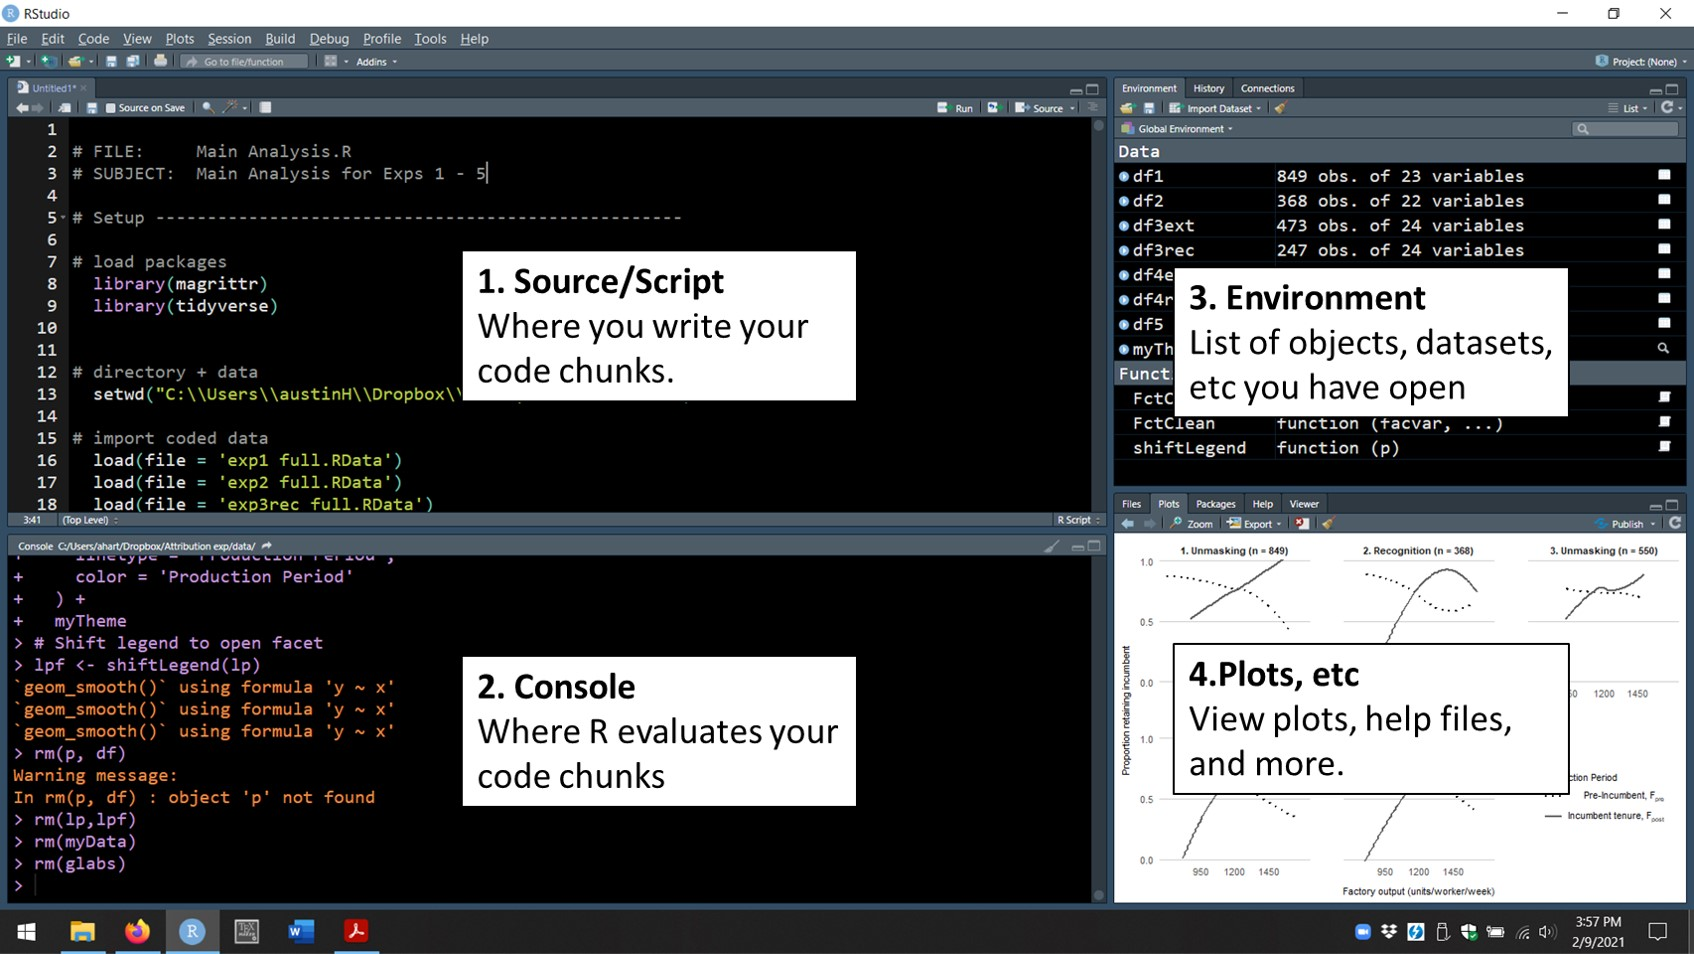
\includegraphics[width=0.75\linewidth]{C:\Users\ahart\Dropbox\SIS 600 AH\quick r survival guide\rstudiowindow} 

}

\caption{RStudio Interface}\label{fig:interface}
\end{figure}

The source pane is where you'll write individual scripts: the collections of R code chunks that constitute your analysis. The console is where R evaluates the code you choose to execute. Each code chunk in the console begins with the symbol \texttt{\textgreater{}}, and the output from each chunk is printed below it. For example, type \texttt{2+10/5} into the console and hit enter.

\begin{Shaded}
\begin{Highlighting}[]
  \DecValTok{2} \SpecialCharTok{+} \DecValTok{10}\SpecialCharTok{/}\DecValTok{5}
\DocumentationTok{\#\# [1] 4}
\end{Highlighting}
\end{Shaded}

The environment pane displays the objects (dataframes, graphs, lists, etc) available. Finally, the plots/help panel displays your graphs, help files, and more. For example, load a built\texttt{-}in data frame and create a simple histogram. Type and execute the code below:

\begin{Shaded}
\begin{Highlighting}[]
\NormalTok{  IrisData }\OtherTok{=}\NormalTok{ iris}

  \FunctionTok{hist}\NormalTok{(IrisData}\SpecialCharTok{$}\NormalTok{Petal.Width)}
\end{Highlighting}
\end{Shaded}

\begin{center}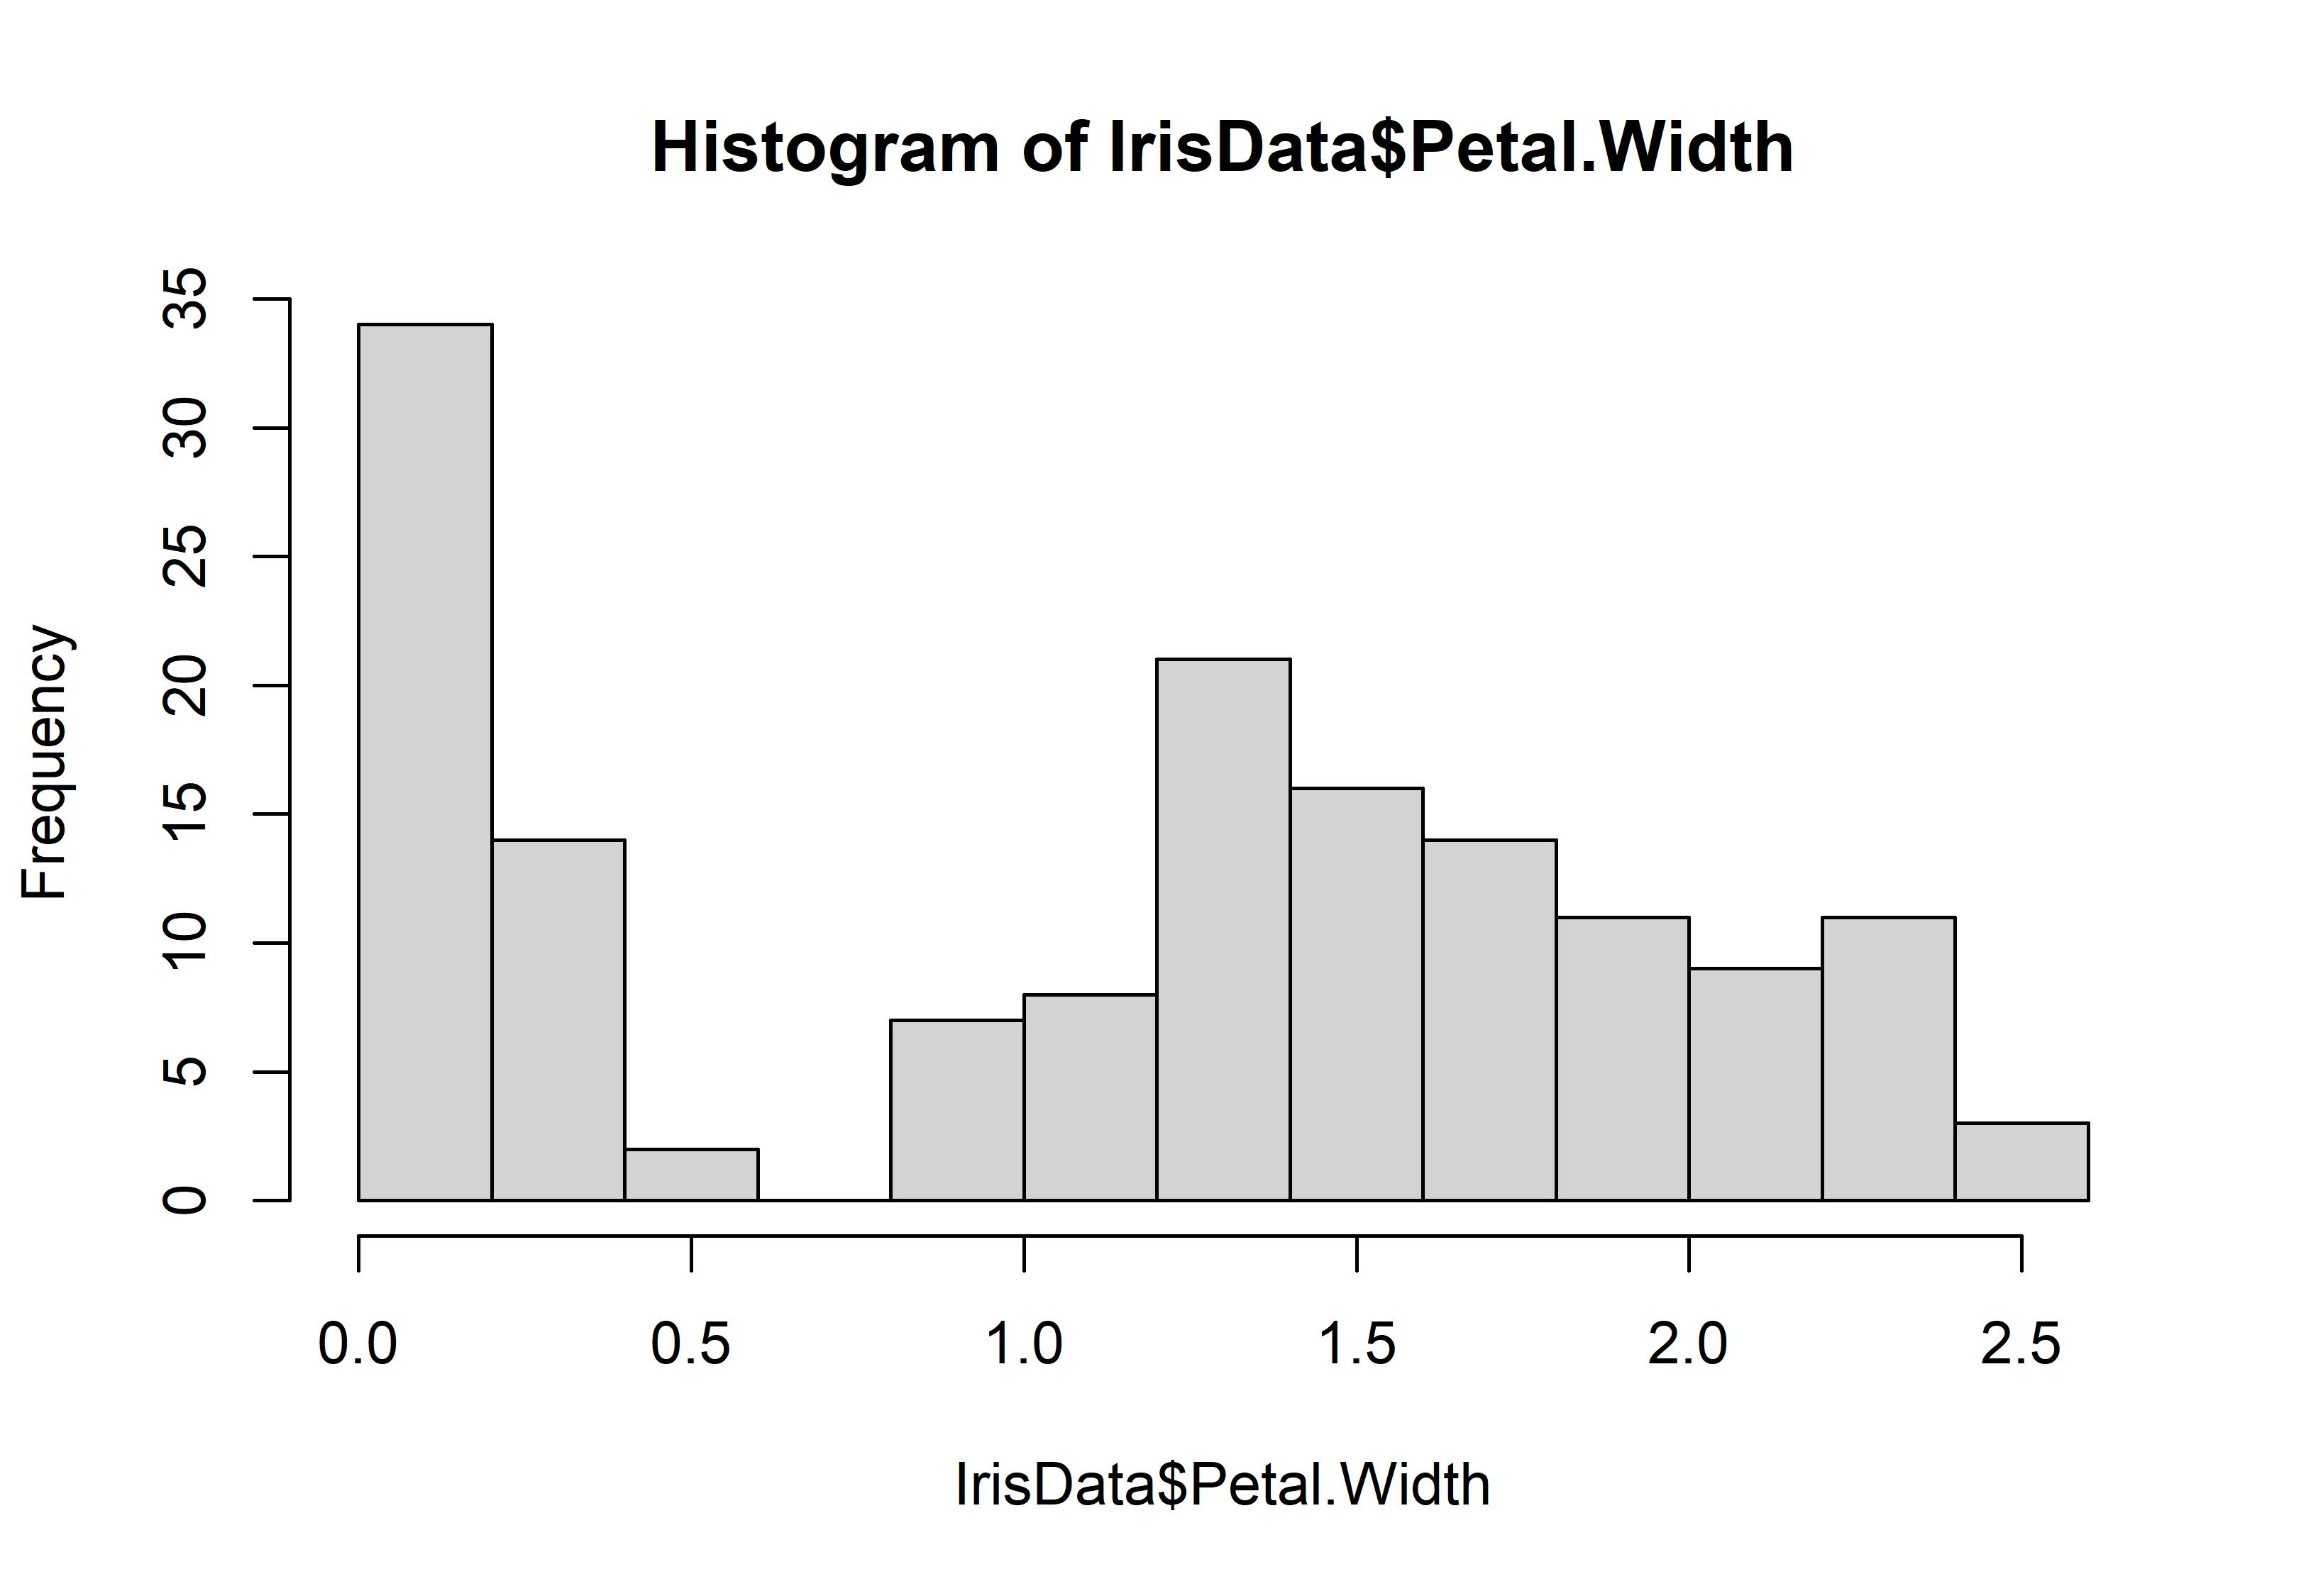
\includegraphics[width=0.4\linewidth]{SurvivR_files/figure-latex/histex-1} \end{center}

Notice that the data frame \texttt{IrisData} is now listed in the environment pane. The histogram is displayed in the plot window.

\hypertarget{code-chunks}{%
\section{Code chunks}\label{code-chunks}}

\hypertarget{writing-and-executing}{%
\subsection{Writing and executing}\label{writing-and-executing}}

Open RStudio, and create a new R Script file (click the icon near the upper left that looks like a piece of paper with a green plus on it). Type the following lines into the script:

\begin{Shaded}
\begin{Highlighting}[]
\NormalTok{  x }\OtherTok{=} \FunctionTok{rnorm}\NormalTok{(}\AttributeTok{n =} \DecValTok{1000}\NormalTok{, }\AttributeTok{mean =} \DecValTok{10}\NormalTok{, }\AttributeTok{sd =} \DecValTok{4}\NormalTok{)}
  \FunctionTok{mean}\NormalTok{(x)}
\DocumentationTok{\#\# [1] 9.931}
\end{Highlighting}
\end{Shaded}

Execute a command from your script by clicking within the line with your mouse (or click on the line number, or click and drag to select multiple lines at once) and clicking Run (Ctrl + Enter). You can execute lines one at a time or as a group. Try executing the lines above. Compare your output:

\begin{verbatim}
## [1] 9.859
\end{verbatim}

\hypertarget{commenting-with}{%
\subsection{Commenting with}\label{commenting-with}}

It's important to add comments throughout your script. These can function as section headers, or as notes to your future self/colleagues on what you were attempting to do. R treats anything after the \texttt{\#} sign as a comment and ignores it when executing commands. For instance:

\begin{Shaded}
\begin{Highlighting}[]
\CommentTok{\# Practice executing commands    }
\NormalTok{  x }\OtherTok{=} \FunctionTok{rnorm}\NormalTok{(}\AttributeTok{n =} \DecValTok{1000}\NormalTok{, }\AttributeTok{mean =} \DecValTok{10}\NormalTok{, }\AttributeTok{sd =} \DecValTok{4}\NormalTok{)  }\CommentTok{\# create a new object, x}
  \FunctionTok{mean}\NormalTok{(x)                                 }\CommentTok{\# calculate the mean of it}
\end{Highlighting}
\end{Shaded}

\hypertarget{installing-packages}{%
\section{Installing packages}\label{installing-packages}}

R's advanced functionality comes from the use of packages--user-defined programs (like apps on a phone) that enable it to carry out particular tasks. We rely largely on a suite of packages called the \texttt{tidyverse}. To install this (or any package), use the command \texttt{install.packages(\textquotesingle{}packageName\textquotesingle{})} in your script. Be sure to include the name of the package in single or double quotes. Note that tidyverse will take several minutes to install:

\begin{Shaded}
\begin{Highlighting}[]
  \FunctionTok{install.packages}\NormalTok{(}\StringTok{\textquotesingle{}tidyverse\textquotesingle{}}\NormalTok{)}
\end{Highlighting}
\end{Shaded}

\hypertarget{loading-packages-for-use}{%
\section{Loading packages for use}\label{loading-packages-for-use}}

You only have to install a package once, but you need to load it in each R session in order to use it. Simply call the desired package using the command \texttt{library(packagename)}. It's a good idea to start any R script by loading frequently-used packages. Especially \texttt{tidyverse}:

\begin{Shaded}
\begin{Highlighting}[]
  \FunctionTok{library}\NormalTok{(tidyverse)}
\end{Highlighting}
\end{Shaded}

Note that you can also call a specific function without loading the entire package that defines it. For example, \texttt{haven::read\_dta()} executes the \texttt{read\_dta()} function from the \texttt{haven} package without loading the package itself.

\hypertarget{setting-a-working-directory}{%
\section{Setting a working directory}\label{setting-a-working-directory}}

Every data project needs a home. Your working directory is the folder on your computer from which R will load data, images, etc and to which it will save your output. It's important to designate your working directory at the beginning of any script using the \texttt{setwd(\textquotesingle{}filepath\textquotesingle{})} command. For example:

\begin{Shaded}
\begin{Highlighting}[]
  \FunctionTok{setwd}\NormalTok{(}\StringTok{\textquotesingle{}C:}\SpecialCharTok{\textbackslash{}\textbackslash{}}\StringTok{Users}\SpecialCharTok{\textbackslash{}\textbackslash{}}\StringTok{ahart}\SpecialCharTok{\textbackslash{}\textbackslash{}}\StringTok{Documents}\SpecialCharTok{\textbackslash{}\textbackslash{}}\StringTok{SIS600\textquotesingle{}}\NormalTok{)}
\end{Highlighting}
\end{Shaded}

This is where you should save the datasets for your project. Note the use of the double backslash, \texttt{\textbackslash{}\textbackslash{}}, when specifying the directory.

If you're unsure about the current directory, check using the \texttt{getwd()} function:

\begin{Shaded}
\begin{Highlighting}[]
  \FunctionTok{getwd}\NormalTok{()}
\end{Highlighting}
\end{Shaded}

\begin{verbatim}
## [1] "C:/Users/ahart/Documents/SIS600"
\end{verbatim}

You can verify that the correct files are there using \texttt{list.files()}:

\begin{Shaded}
\begin{Highlighting}[]
  \FunctionTok{list.files}\NormalTok{()}
\end{Highlighting}
\end{Shaded}

\begin{verbatim}
## [1] "biopics.xls"        "DCPS testing.RData"
\end{verbatim}

\hypertarget{getting-help-with-r}{%
\section{Getting help with R}\label{getting-help-with-r}}

Documentation within R is sometimes helpful, sometimes less so. To see the help file for a given command, enter \texttt{help(command)}, or (equivalently) \texttt{?command}. These will bring up a tutorial with a basic description, usage, arguments, syntax, and other notes about the command. For example, to get help with setting a working directory:

\begin{Shaded}
\begin{Highlighting}[]
  \FunctionTok{help}\NormalTok{(setwd)}
\NormalTok{  ?setwd}
\end{Highlighting}
\end{Shaded}

If that fails, ask the internet by searching Google or \url{https://rseek.org/}, a search engine dedicated specifically to results about R.

\hypertarget{basics-of-r-programming}{%
\chapter{Basics of R Programming}\label{basics-of-r-programming}}

\hypertarget{thinking-like-r}{%
\section{Thinking like R}\label{thinking-like-r}}

R is built in the paradigm of Object-Oriented Programming. It uses a system of objects (which contain information) and functions that operate on objects (by manipulating them in a certain way, extracting information from or about them, calculating statistics or plotting graphs based on their data, etc). Objects are identified by names, which must start with a letter, not overwrite an already-defined object, and not include any spaces.

\hypertarget{objects}{%
\section{Objects}\label{objects}}

Objects are created by assigning them a value using the object name, followed by an assignment operator (i.e.~\texttt{=} or \texttt{\textless{}-}), followed by either the information they should contain or instructions for importing information from another file. Entering information without assigning it to an object simply prints the output to the console; by assigning it a name it is possible to work with it.

\begin{Shaded}
\begin{Highlighting}[]
  \DecValTok{1}\SpecialCharTok{:}\DecValTok{4}               \CommentTok{\# prints a sequence of integers}
\DocumentationTok{\#\# [1] 1 2 3 4}
     
\NormalTok{  MyObject }\OtherTok{=} \DecValTok{1}\SpecialCharTok{:}\DecValTok{4}    \CommentTok{\# assigns the sequence to a new object, myObject}
\end{Highlighting}
\end{Shaded}

To report the contents of an object, enter the object name on a line and execute that line.

\begin{Shaded}
\begin{Highlighting}[]
\NormalTok{  MyObject}
\end{Highlighting}
\end{Shaded}

\begin{verbatim}
## [1] 1 2 3 4
\end{verbatim}

Objects no longer needed can be removed from the workspace using \texttt{remove()} In this case:

\begin{Shaded}
\begin{Highlighting}[]
  \FunctionTok{remove}\NormalTok{(MyObject)}
\end{Highlighting}
\end{Shaded}

\hypertarget{functions-in-r}{%
\section{Functions in R}\label{functions-in-r}}

Functions operate on objects. Call on a function by using the name of the function followed by parenthesis, within which are the arguments the function takes, i.e.~\texttt{SomeFunction(args)}. Each function has its own set of arguments that tell it what object(s) to act on and what to do with them.

For example: the concatenate function \texttt{c(item1,item2,...)} combines a series of elements into a single (vector) object, and takes as its arguments the elements to be included.

\begin{Shaded}
\begin{Highlighting}[]
  \FunctionTok{c}\NormalTok{(}\DecValTok{1}\NormalTok{,}\DecValTok{2}\NormalTok{,}\DecValTok{3}\NormalTok{,}\DecValTok{4}\NormalTok{)   }\CommentTok{\# combine integers}
\DocumentationTok{\#\# [1] 1 2 3 4}

\NormalTok{  a }\OtherTok{=} \DecValTok{1}\SpecialCharTok{:}\DecValTok{4}        \CommentTok{\# create new objects, a and b         }
\NormalTok{  b }\OtherTok{=} \DecValTok{5}\SpecialCharTok{:}\DecValTok{7}
  
  \FunctionTok{c}\NormalTok{(a,b)         }\CommentTok{\# combine objects}
\DocumentationTok{\#\# [1] 1 2 3 4 5 6 7}
\end{Highlighting}
\end{Shaded}

\hypertarget{the-pipe-operator}{%
\section{The Pipe Operator}\label{the-pipe-operator}}

The pipe operator \texttt{\%\textgreater{}\%} from the \texttt{tidyverse} package strings together a series of functions into a single command. It will take the output from the first function and use it as the input for the second, take the output from the second as input for the third, etc. For example, creating a sequence from 0 to 100 with intervals of 2, calculating the sum of these numbers, and calculating (and printing) the square root of this sum, can be done in three ways.

\begin{Shaded}
\begin{Highlighting}[]
\NormalTok{  a }\OtherTok{=} \FunctionTok{seq}\NormalTok{(}\DecValTok{0}\NormalTok{,}\DecValTok{100}\NormalTok{,}\DecValTok{2}\NormalTok{) }
\NormalTok{  b }\OtherTok{=} \FunctionTok{sum}\NormalTok{(a)}
\NormalTok{  c }\OtherTok{=} \FunctionTok{sqrt}\NormalTok{(b)}
\NormalTok{  c}
\DocumentationTok{\#\# [1] 50.5}
     
  \FunctionTok{sqrt}\NormalTok{(}\FunctionTok{sum}\NormalTok{(}\FunctionTok{seq}\NormalTok{(}\DecValTok{0}\NormalTok{,}\DecValTok{100}\NormalTok{,}\DecValTok{2}\NormalTok{)))}
\DocumentationTok{\#\# [1] 50.5}

  \FunctionTok{seq}\NormalTok{(}\DecValTok{0}\NormalTok{,}\DecValTok{100}\NormalTok{,}\DecValTok{2}\NormalTok{) }\SpecialCharTok{\%\textgreater{}\%}   \CommentTok{\# pipes the sequence forward   }
    \FunctionTok{sum}\NormalTok{() }\SpecialCharTok{\%\textgreater{}\%}        \CommentTok{\# take the sum of the sequence; pipe forward }
    \FunctionTok{sqrt}\NormalTok{()           }\CommentTok{\# square root}
\DocumentationTok{\#\# [1] 50.5}
\end{Highlighting}
\end{Shaded}

The pipe operator becomes a very useful feature as you move to performing complex, multi-step operations. It allows carrying out a series of manipulations to an object without having to create a new named object each step of the way, or getting lost in endless nesting of parentheses within a command.

\hypertarget{working-with-data}{%
\chapter{Working with data}\label{working-with-data}}

Typically, a dataset will take the form of a data frame (or a tibble) where each column is a vector representing a single variable and each row (i.e.~each corresponding position within those vectors) represents a single observation. Each element, then, is the value a particular observation takes on for that particular variable.

\hypertarget{importing-data}{%
\section{Importing data}\label{importing-data}}

One of the biggest challenges for first-time \texttt{R} users is importing a dataset. Though the process is similar, the specific functions for loading data depend on the format of your data. Here we cover how to import the most common types of data files.

\hypertarget{r-data-.rdata}{%
\subsection{R data (.rdata)}\label{r-data-.rdata}}

The file extension for a data frame saved in \texttt{R} is \texttt{.RData}. An object can be opened using the \texttt{load(\textquotesingle{}filename\textquotesingle{})} command. Test this out by loading the \texttt{DCPS\ testing} data.

\begin{Shaded}
\begin{Highlighting}[]
  \FunctionTok{load}\NormalTok{(}\StringTok{\textquotesingle{}DCPS testing.RData\textquotesingle{}}\NormalTok{)}
\end{Highlighting}
\end{Shaded}

Note that this works only if the dataset is saved in the working directory. If not, you need to specify the complete file path here.

\hypertarget{delimited-.csv-files}{%
\subsection{Delimited (.csv) files}\label{delimited-.csv-files}}

Often the datasets you work with will not be in \texttt{.rdata} format, or it will be more convenient to store them in another format so that you can create or work with them using other software. The simplest option is to work with Comma-Separated Values (.csv) files. To import data from a \texttt{.csv} file, use the \texttt{read\_csv(\textquotesingle{}filename\textquotesingle{})} function defined within \texttt{tidyverse}.

\begin{Shaded}
\begin{Highlighting}[]
\NormalTok{  myCSV }\OtherTok{\textless{}{-}} \FunctionTok{read\_csv}\NormalTok{(}\StringTok{\textquotesingle{}csvData.csv\textquotesingle{}}\NormalTok{)}
\end{Highlighting}
\end{Shaded}

\hypertarget{excel-.xls-.xlsx-files}{%
\subsection{Excel (.xls, .xlsx) files}\label{excel-.xls-.xlsx-files}}

To import data from Excel (\texttt{.xlsx} or \texttt{.xls}), use the \texttt{read\_excel(\textquotesingle{}filename\textquotesingle{})} function defined in the \texttt{readxl} package. Note that \texttt{readxl} installs automatically with the \texttt{tidyverse}, but you have to load it separately. Practice this command by loading the \texttt{biopic.xls} data required for this guide.

\begin{Shaded}
\begin{Highlighting}[]
  \FunctionTok{library}\NormalTok{(readxl)}

\NormalTok{  film }\OtherTok{\textless{}{-}} \FunctionTok{read\_excel}\NormalTok{(}\StringTok{\textquotesingle{}biopics.xls\textquotesingle{}}\NormalTok{)}
\end{Highlighting}
\end{Shaded}

If it does not load, verify that the dataset is saved in your working directory.

\hypertarget{stata-.dta-or-spss-.sav-files}{%
\subsection{Stata (.dta) or SPSS (.sav) files}\label{stata-.dta-or-spss-.sav-files}}

To import datafiles written in Stata (\texttt{.dta}) or SPSS (\texttt{.sav}), we rcommend using the \texttt{read\_dta(\textquotesingle{}filename\textquotesingle{})} and \texttt{read\_spss(\textquotesingle{}filename\textquotesingle{})} functions defined in the \texttt{haven} package. Note that \texttt{haven} is part of the \texttt{tidyverse}, but you must load it separately.

\begin{Shaded}
\begin{Highlighting}[]
  \FunctionTok{library}\NormalTok{(haven)}

\NormalTok{  myStata }\OtherTok{\textless{}{-}} \FunctionTok{read\_dta}\NormalTok{(}\StringTok{\textquotesingle{}stataData.dta\textquotesingle{}}\NormalTok{) }\CommentTok{\# Stata format}
\NormalTok{  mySPSS }\OtherTok{\textless{}{-}} \FunctionTok{read\_spss}\NormalTok{(}\StringTok{\textquotesingle{}spssData.sav\textquotesingle{}}\NormalTok{) }\CommentTok{\# SPSS format}
\end{Highlighting}
\end{Shaded}

\hypertarget{a-first-look-at-your-data}{%
\section{A first look at your data}\label{a-first-look-at-your-data}}

You can use the \texttt{names()} function to see a list of variables (names and column number) in your data frame.

Use the \texttt{head()} function to preview the first rows of a data frame.

To view the entire data frame, either click on the object in the ``Data'' window or use \texttt{View()}.

\begin{Shaded}
\begin{Highlighting}[]
  \FunctionTok{names}\NormalTok{(dcps)  }\CommentTok{\# identify variable names}
\DocumentationTok{\#\# [1] "SchCode"     "SchName"     "SchType"    }
\DocumentationTok{\#\# [4] "NumTested"   "ProfLang"    "ProfMath"   }
\DocumentationTok{\#\# [7] "DataVERSION"}

  \FunctionTok{head}\NormalTok{(dcps)   }\CommentTok{\# see the first few rows of data}
\DocumentationTok{\#\# \# A tibble: 6 x 7}
\DocumentationTok{\#\#   SchCode SchName SchType NumTested ProfLang ProfMath}
\DocumentationTok{\#\#     \textless{}dbl\textgreater{} \textless{}chr\textgreater{}   \textless{}fct\textgreater{}       \textless{}dbl\textgreater{}    \textless{}dbl\textgreater{}    \textless{}dbl\textgreater{}}
\DocumentationTok{\#\# 1     202 Aiton \textasciitilde{} Elemen\textasciitilde{}        72     5.56   15.3  }
\DocumentationTok{\#\# 2     203 Amidon\textasciitilde{} Elemen\textasciitilde{}       147    16.3    10.1  }
\DocumentationTok{\#\# 3     450 Anacos\textasciitilde{} High           67     4.48    1.43 }
\DocumentationTok{\#\# 4     452 Ballou\textasciitilde{} High          180     2.78    0.498}
\DocumentationTok{\#\# 5     204 Bancro\textasciitilde{} Elemen\textasciitilde{}       213    34.3    39.9  }
\DocumentationTok{\#\# 6     205 Barnar\textasciitilde{} Elemen\textasciitilde{}       224    38.4    39.7  }
\DocumentationTok{\#\# \# ... with 1 more variable: DataVERSION \textless{}chr\textgreater{}}
\end{Highlighting}
\end{Shaded}

\hypertarget{referencing-variables-of-a-data-frame}{%
\section{Referencing variables of a data frame}\label{referencing-variables-of-a-data-frame}}

A data frame (or tibble) is a two-dimensional structure in which each variable forms a column and each observation forms a row. Each element is the value that a given observation takes on for a particular variable.

How do you reference or identify the variables in a data frame (e.g.~to calculate the mean number of students tested, \texttt{NumTested} from the \texttt{dcps} schools data)? The \texttt{\$} and \texttt{{[}{[}} extraction operators both pull variables from a dataframe or items from a list. Note that \texttt{\$} requires the variable name, whereas \texttt{{[}{[}} allows you to use either the variable's name (in quotes) or column number in the data frame. Do what you want. I prefer \texttt{{[}{[}} for anyone in more advanced programming, but I'll typically use \texttt{\$} in this course.

\begin{Shaded}
\begin{Highlighting}[]
\CommentTok{\# Extract the variable (all observations)}
\NormalTok{  dcps}\SpecialCharTok{$}\NormalTok{NumTested}
\DocumentationTok{\#\#   [1]   72  147   67  180  213  224  158  112  157  375}
\DocumentationTok{\#\#  [11]  222  149  167   67   83   87   96  121  289  109}
\DocumentationTok{\#\#  [21]  495   62 1423  146  117  156  109  189  212  159}
\DocumentationTok{\#\#  [31]  112   77  137  112  362  310  110  160   94   91}
\DocumentationTok{\#\#  [41]  178  334  290  235  354  114  156  137  115  181}
\DocumentationTok{\#\#  [51]  306  111   96  193  246  132   12  129   93  153}
\DocumentationTok{\#\#  [61]  143  140  212  143  105  148  258  129   66  144}
\DocumentationTok{\#\#  [71]  399  133  117   79  144  213  120  288   96  170}
\DocumentationTok{\#\#  [81]   20   61  121  261  135  102  113  134  121   73}
\DocumentationTok{\#\#  [91]  217  211  175  409  239  126  102  374  199  180}
\DocumentationTok{\#\# [101]  173  190   23  253  172  154  152  421}

\CommentTok{\# Mean on a variable (3 ways)}
  \FunctionTok{mean}\NormalTok{(dcps}\SpecialCharTok{$}\NormalTok{NumTested) }\CommentTok{\# object$variable}
\DocumentationTok{\#\# [1] 180.1}
  
  \FunctionTok{mean}\NormalTok{(dcps[[}\StringTok{\textquotesingle{}NumTested\textquotesingle{}}\NormalTok{]]) }\CommentTok{\# object[[\textquotesingle{}variable\textquotesingle{}]]}
\DocumentationTok{\#\# [1] 180.1}
  
  \FunctionTok{mean}\NormalTok{(dcps[[}\DecValTok{4}\NormalTok{]]) }\CommentTok{\# object[[column\#]]}
\DocumentationTok{\#\# [1] 180.1}
\end{Highlighting}
\end{Shaded}

\hypertarget{saving-your-work}{%
\section{Saving your work}\label{saving-your-work}}

Always save your work! Early and often! This is true both of both your scripts and your datasets. R will ask if you want to save your ``workspace'' when you close the session, and you should not. Save your script instead.

\hypertarget{saving-an-r-script}{%
\subsection{Saving an R script}\label{saving-an-r-script}}

To save you \texttt{.r} script file in \texttt{RStudio}, go to File - Save (or Save As\ldots).

\hypertarget{saving-a-data-frame}{%
\subsection{Saving a data frame}\label{saving-a-data-frame}}

To save a data frame as a \texttt{.rdata} data file, use the \texttt{save(object,\textquotesingle{}filename\textquotesingle{})} command. To save a data frame as (i.e.~write it onto) a \texttt{.csv} file, use the \texttt{write\_csv(object,\ \textquotesingle{}filename\textquotesingle{})} command and enter the name of the object and the file name.

\begin{Shaded}
\begin{Highlighting}[]
  \FunctionTok{save}\NormalTok{(myData, }\AttributeTok{file =} \StringTok{\textquotesingle{}sampledata.rdata\textquotesingle{}}\NormalTok{)      }\CommentTok{\# to save as an Rdata file}

  \FunctionTok{write\_csv}\NormalTok{(myData, }\AttributeTok{file =} \StringTok{\textquotesingle{}sampledata.csv\textquotesingle{}}\NormalTok{)   }\CommentTok{\# to write onto a .csv file}
\end{Highlighting}
\end{Shaded}

As always, these actions will write the new file to your working directory. If you have not specified a working directory, or if you want to save elsewehere, specify the complete path name here.

\hypertarget{descriptive-statistics}{%
\chapter{Descriptive statistics}\label{descriptive-statistics}}

How do you summarize numeric data (continuous or discrete) and present your findings? Here we cover how to analyze data over a single numeric variable, both in isolation (e.g.~basic summary statistics) and across discrete categories of another variable (e.g.~group mean comparison).

Note that you will need the \texttt{dcps} data (\texttt{DCPS\ testing.RData}) to replicate the examples in this chapter.

\hypertarget{describing-one-variable}{%
\section{Describing one variable}\label{describing-one-variable}}

\hypertarget{summary-statistics}{%
\subsection{Summary statistics}\label{summary-statistics}}

A useful first step in analyzing the distribution of scores on a single numeric variable is to calculate the relevant summary statistics. Use the \texttt{summary()} function for a quick, general overview. This returns the minimum, mean, and maximum scores, as well as the score at 1st, 2nd (median), and 3rd quartiles.

\begin{Shaded}
\begin{Highlighting}[]
  \FunctionTok{summary}\NormalTok{(dcps)  }\CommentTok{\# for every variable in the data frame}
\DocumentationTok{\#\#     SchCode      SchName                SchType  }
\DocumentationTok{\#\#  Min.   :202   Length:108         Elementary:64  }
\DocumentationTok{\#\#  1st Qu.:264   Class :character   Middle    :25  }
\DocumentationTok{\#\#  Median :318   Mode  :character   High      :19  }
\DocumentationTok{\#\#  Mean   :340                                     }
\DocumentationTok{\#\#  3rd Qu.:414                                     }
\DocumentationTok{\#\#  Max.   :943                                     }
\DocumentationTok{\#\#    NumTested       ProfLang       ProfMath    }
\DocumentationTok{\#\#  Min.   :  12   Min.   : 0.0   Min.   : 0.00  }
\DocumentationTok{\#\#  1st Qu.: 112   1st Qu.:12.3   1st Qu.: 9.38  }
\DocumentationTok{\#\#  Median : 146   Median :19.1   Median :20.56  }
\DocumentationTok{\#\#  Mean   : 180   Mean   :29.7   Mean   :26.96  }
\DocumentationTok{\#\#  3rd Qu.: 212   3rd Qu.:40.0   3rd Qu.:36.88  }
\DocumentationTok{\#\#  Max.   :1423   Max.   :94.1   Max.   :82.76  }
\DocumentationTok{\#\#  DataVERSION       }
\DocumentationTok{\#\#  Length:108        }
\DocumentationTok{\#\#  Class :character  }
\DocumentationTok{\#\#  Mode  :character  }
\DocumentationTok{\#\#                    }
\DocumentationTok{\#\#                    }
\DocumentationTok{\#\# }

  \FunctionTok{summary}\NormalTok{(dcps}\SpecialCharTok{$}\NormalTok{ProfLang) }\CommentTok{\# for a specific variable}
\DocumentationTok{\#\#    Min. 1st Qu.  Median    Mean 3rd Qu.    Max. }
\DocumentationTok{\#\#     0.0    12.3    19.1    29.7    40.0    94.1}
\end{Highlighting}
\end{Shaded}

For specific inquiries, use the \texttt{summarize()} function and customize your report. For example:

\begin{Shaded}
\begin{Highlighting}[]
\NormalTok{  dcps }\SpecialCharTok{\%\textgreater{}\%}   \CommentTok{\# start by piping in the dataset}
    \FunctionTok{summarize}\NormalTok{(}
      \AttributeTok{Avg =} \FunctionTok{mean}\NormalTok{(ProfLang), }\CommentTok{\# calculates the mean}
      \AttributeTok{StdDev =} \FunctionTok{sd}\NormalTok{(ProfLang),   }\CommentTok{\# standard deviation}
      \AttributeTok{Range =} \FunctionTok{max}\NormalTok{(ProfLang) }\SpecialCharTok{{-}} \FunctionTok{min}\NormalTok{(ProfLang) }
\NormalTok{    )}
\DocumentationTok{\#\# \# A tibble: 1 x 3}
\DocumentationTok{\#\#     Avg StdDev Range}
\DocumentationTok{\#\#   \textless{}dbl\textgreater{}  \textless{}dbl\textgreater{} \textless{}dbl\textgreater{}}
\DocumentationTok{\#\# 1  29.7   24.6  94.1}
\end{Highlighting}
\end{Shaded}

\hypertarget{graphing-the-distribution}{%
\subsection{Graphing the distribution}\label{graphing-the-distribution}}

We typically use a histogram or box plot to visualize the distribution of scores on a numeric variable.

\begin{Shaded}
\begin{Highlighting}[]
\CommentTok{\# Basic histogram}
  \FunctionTok{hist}\NormalTok{(dcps}\SpecialCharTok{$}\NormalTok{ProfLang)}
\end{Highlighting}
\end{Shaded}

\begin{center}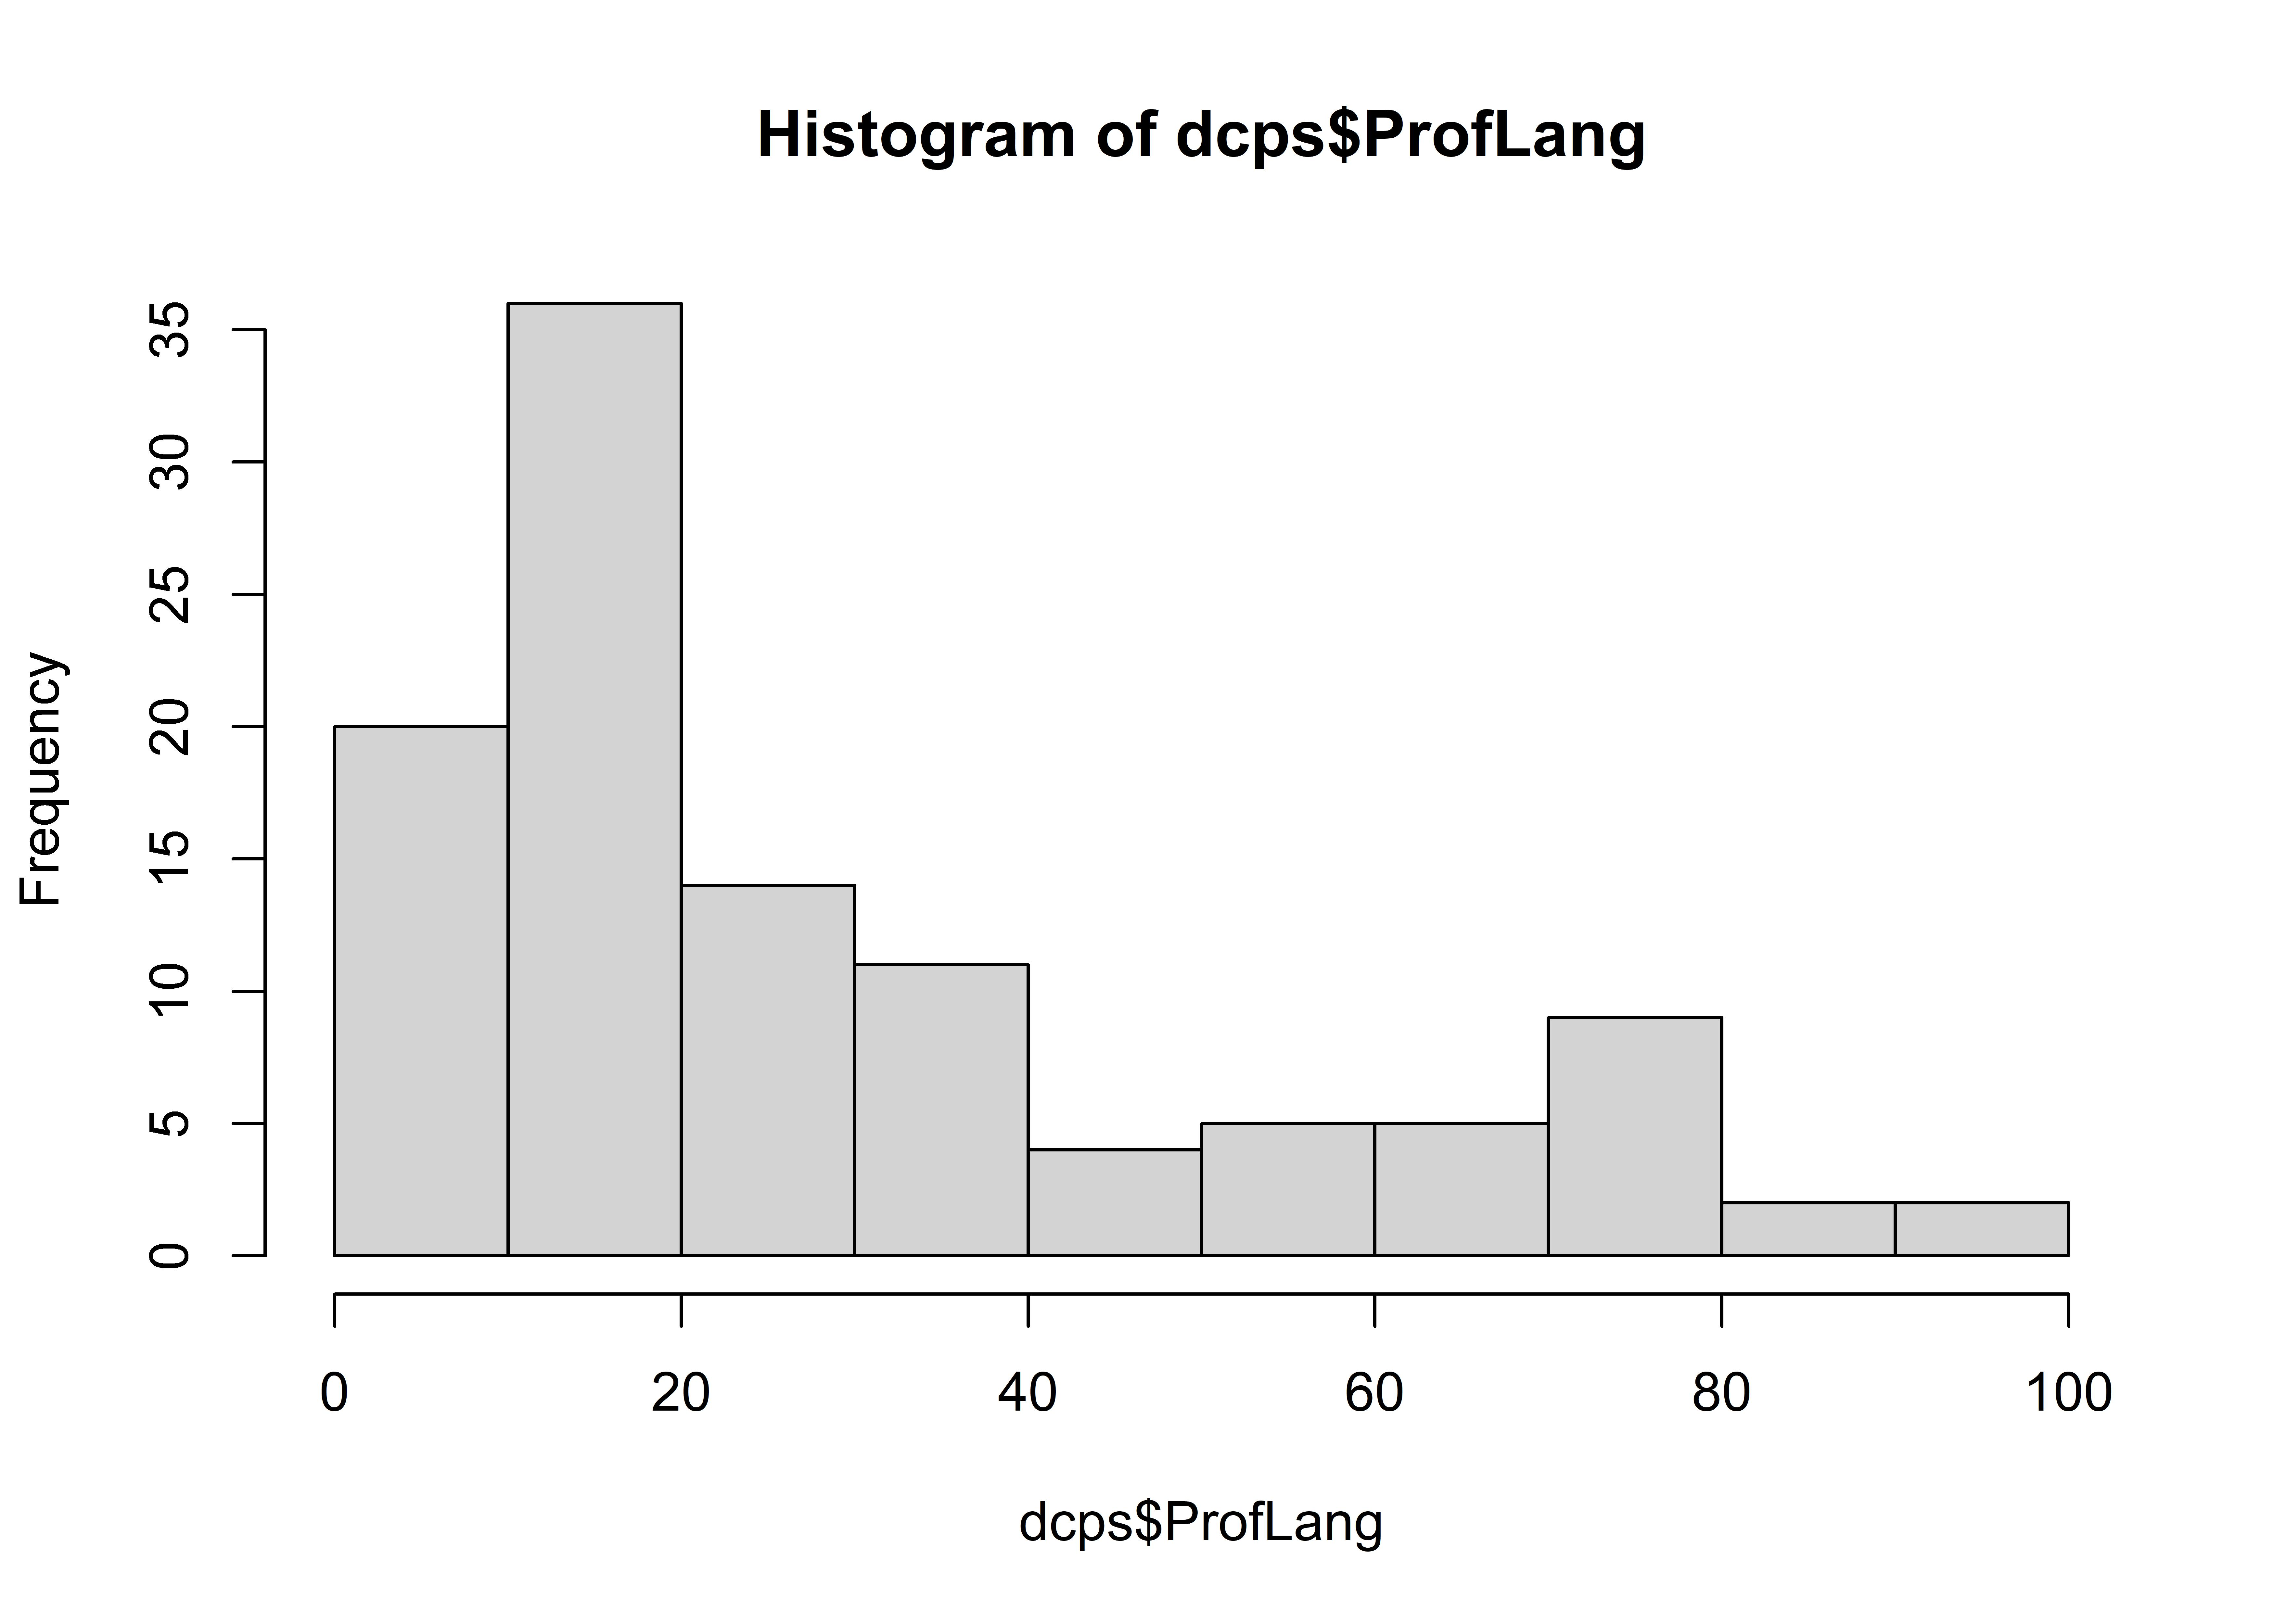
\includegraphics[width=0.4\linewidth]{SurvivR_files/figure-latex/descPlots-1} \end{center}

\begin{Shaded}
\begin{Highlighting}[]

\CommentTok{\# Basic boxplot}
  \FunctionTok{boxplot}\NormalTok{(dcps}\SpecialCharTok{$}\NormalTok{ProfLang, }\AttributeTok{horizontal =} \ConstantTok{TRUE}\NormalTok{)}
\end{Highlighting}
\end{Shaded}

\begin{center}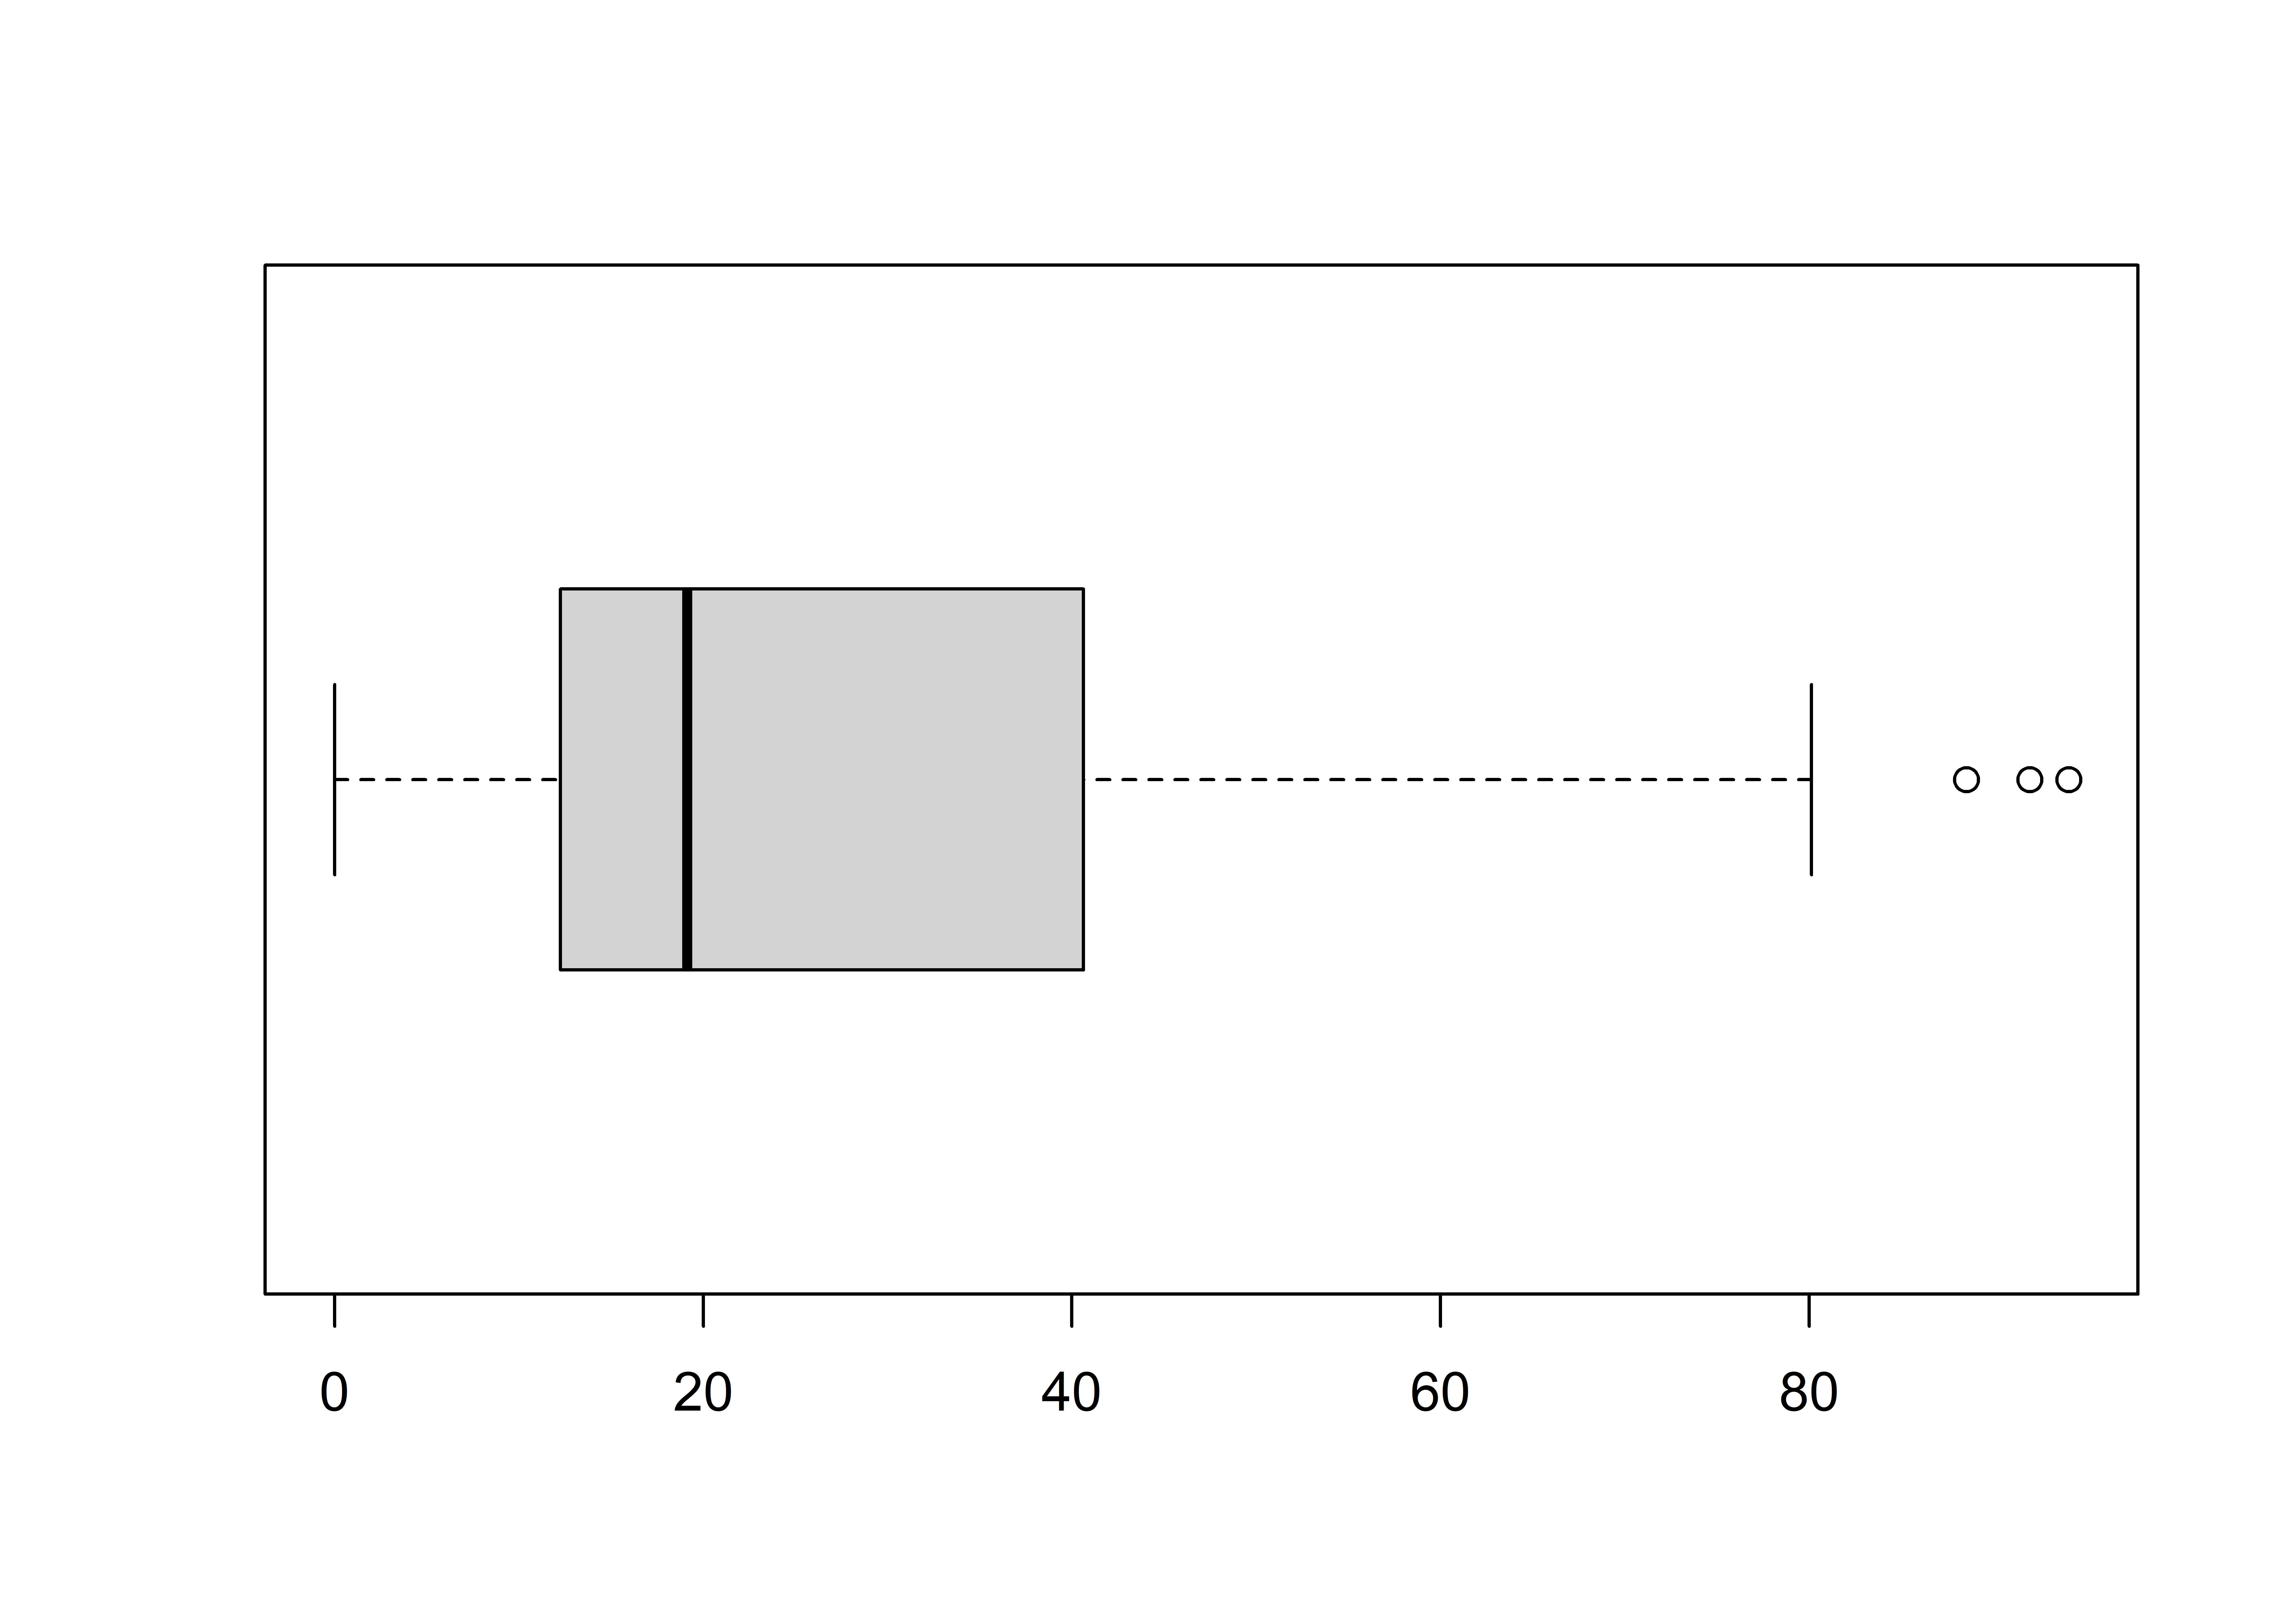
\includegraphics[width=0.4\linewidth]{SurvivR_files/figure-latex/descPlots-2} \end{center}

See the chapter on data visualization to learn how to format these graphs appropriately for academic or professional settings.

\hypertarget{testing-hypotheses}{%
\subsection{Testing hypotheses}\label{testing-hypotheses}}

A one-sample \(t-\)test (\texttt{t.test()}) compares the observed mean on a numeric variable to a hypothesized mean. The resulting \(p\)-value indicates the probability of observing the mean in your data from a population defined by the null hypothesis (\texttt{mu\ =}).

For example, evaluate the argument that at least half of DC public school pupils read at or above grade level (i.e.~\(H_0:~\mu \geq 50\)).

\begin{Shaded}
\begin{Highlighting}[]
  \FunctionTok{t.test}\NormalTok{(dcps}\SpecialCharTok{$}\NormalTok{ProfLang, }\AttributeTok{mu =} \DecValTok{50}\NormalTok{, }\AttributeTok{alternative =} \StringTok{\textquotesingle{}less\textquotesingle{}}\NormalTok{)}
\end{Highlighting}
\end{Shaded}

\begin{verbatim}
## 
##  One Sample t-test
## 
## data:  dcps$ProfLang
## t = -8.6, df = 107, p-value = 5e-14
## alternative hypothesis: true mean is less than 50
## 95 percent confidence interval:
##   -Inf 33.66
## sample estimates:
## mean of x 
##     29.73
\end{verbatim}

The test results suggest that it is extremely unlikely (\(t=-8.6\), \(p<0.001\)) that we would observe these data if the majority of DC public school pupils read at or above grade level. We can reject the null hypothesis.

\hypertarget{omitting-missing-values}{%
\section{Omitting missing values}\label{omitting-missing-values}}

If some observations have missing data (coded \texttt{NA}) on a given variable, summary statistic functions may yield an error. To ignore any missing values in carrying out calculations, include the argument \texttt{na.rm=TRUE} in the function.

\begin{Shaded}
\begin{Highlighting}[]

\NormalTok{  a }\OtherTok{=} \FunctionTok{c}\NormalTok{(}\DecValTok{1}\NormalTok{,}\DecValTok{3}\NormalTok{,}\DecValTok{5}\NormalTok{,}\ConstantTok{NA}\NormalTok{,}\DecValTok{7}\NormalTok{)}

  \FunctionTok{mean}\NormalTok{(a) }\CommentTok{\# Operation fails}
\DocumentationTok{\#\# [1] NA}
  
  \FunctionTok{mean}\NormalTok{(a, }\AttributeTok{na.rm =} \ConstantTok{TRUE}\NormalTok{) }\CommentTok{\# Successfully calculates the mean}
\DocumentationTok{\#\# [1] 4}
\end{Highlighting}
\end{Shaded}

\hypertarget{group-comparisons}{%
\section{Group comparisons}\label{group-comparisons}}

\hypertarget{summary-statistics-by-group}{%
\subsection{Summary statistics by group}\label{summary-statistics-by-group}}

Comparing summary statistics across different groups or categories of cases requires that you identify the grouping variable (typically \texttt{group\_by()}\} before calculating the desired summary statistics.

\begin{Shaded}
\begin{Highlighting}[]
\NormalTok{  dcps }\SpecialCharTok{\%\textgreater{}\%}
    \FunctionTok{group\_by}\NormalTok{(SchType) }\SpecialCharTok{\%\textgreater{}\%}  \CommentTok{\# identify grouping variable}
    \FunctionTok{summarize}\NormalTok{(}
      \AttributeTok{Avg =} \FunctionTok{mean}\NormalTok{(ProfMath),  }\CommentTok{\# apply functions to each group}
      \AttributeTok{StDev =} \FunctionTok{sd}\NormalTok{(ProfMath)}
\NormalTok{    )}
\end{Highlighting}
\end{Shaded}

\begin{verbatim}
## # A tibble: 3 x 3
##   SchType      Avg StDev
## * <fct>      <dbl> <dbl>
## 1 Elementary  34.0  23.7
## 2 Middle      19.6  17.6
## 3 High        12.9  22.5
\end{verbatim}

\hypertarget{visualize-group-differences}{%
\subsection{Visualize group differences}\label{visualize-group-differences}}

One good way of exploring these relationships graphically is to use a boxplot. Note that the syntax is to identify the outcome before the \texttt{\textasciitilde{}} and the grouping variable after (\texttt{boxplot(OutcomeVar\ \textasciitilde{}\ GroupVar,\ Data)}):

\begin{Shaded}
\begin{Highlighting}[]
  \FunctionTok{boxplot}\NormalTok{(ProfMath }\SpecialCharTok{\textasciitilde{}}\NormalTok{ SchType, }\AttributeTok{data =}\NormalTok{ dcps)}
\end{Highlighting}
\end{Shaded}

\begin{center}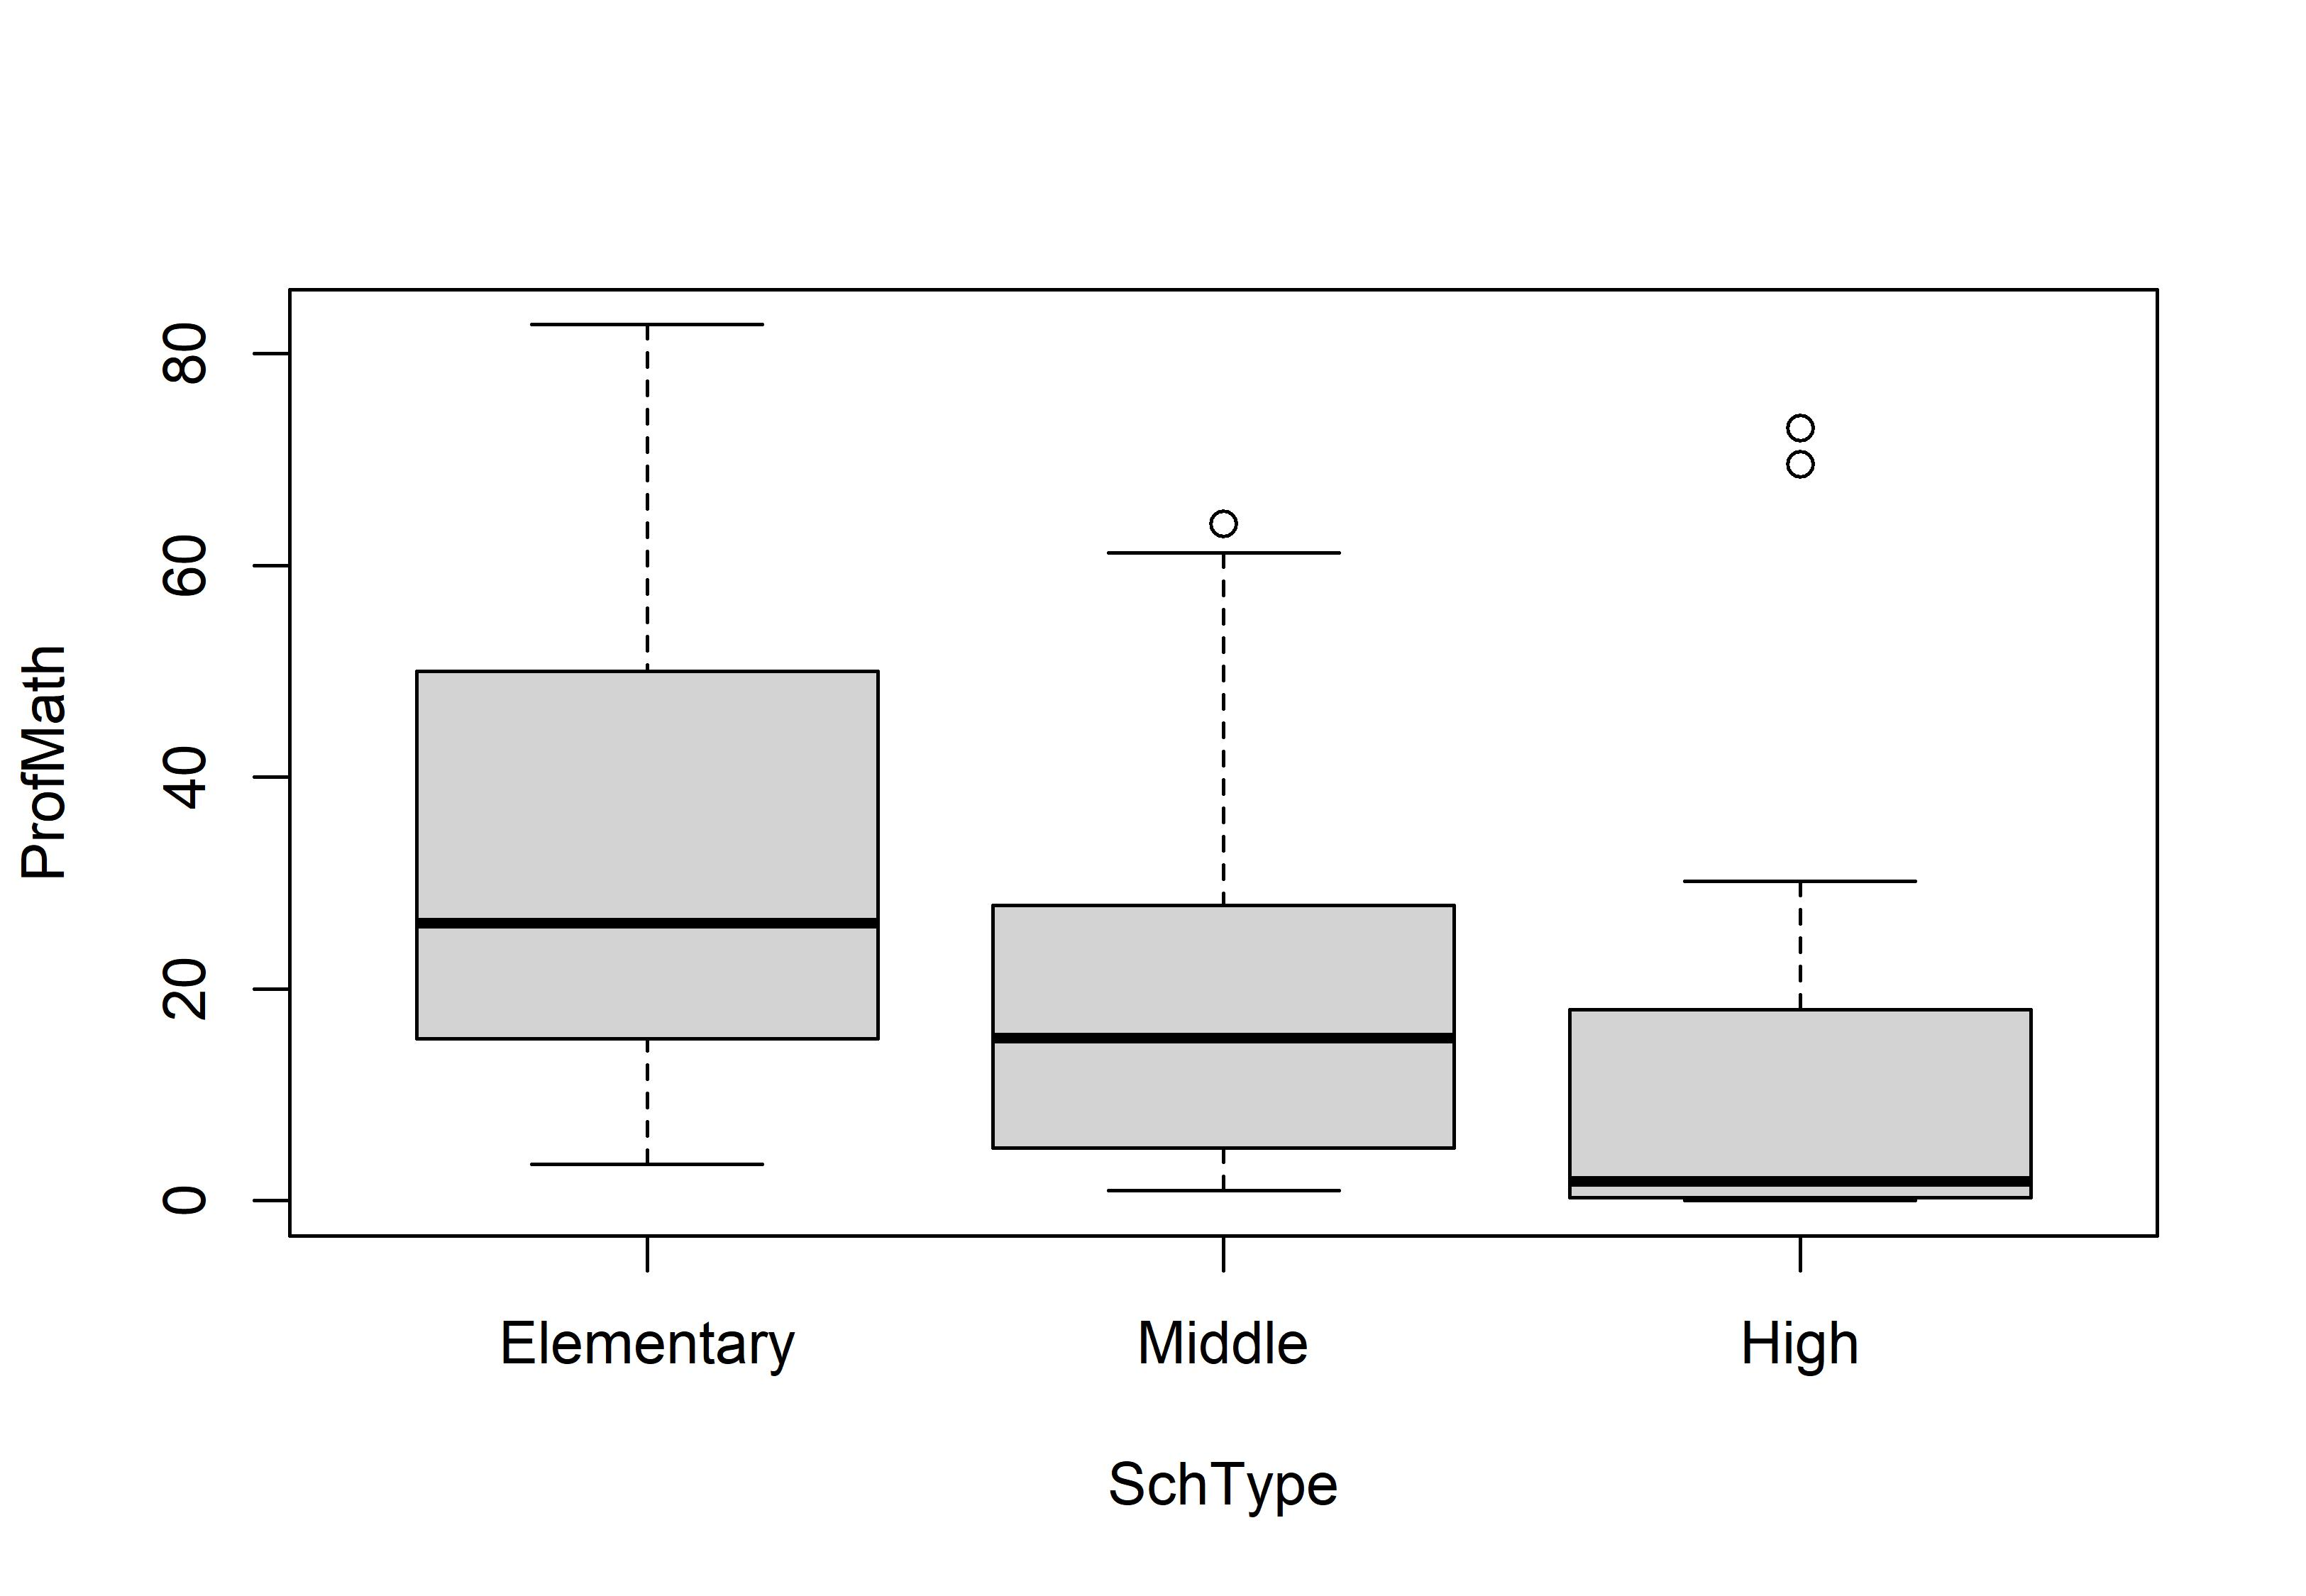
\includegraphics[width=0.4\linewidth]{SurvivR_files/figure-latex/groupbox-1} \end{center}

\hypertarget{testing-hypotheses-1}{%
\subsection{Testing hypotheses}\label{testing-hypotheses-1}}

You can test hypotheses about the relationship between a nominal exposure variable (\texttt{GroupingVar}) and a numeric outcome (\texttt{OutcomeVar}) using either the \(t-\) or \(F-\) test. Use \texttt{t.test(OutcomeVar\ \textasciitilde{}\ GroupVar,\ Data)} to compare the mean outcome across exactly two groups (i.e.~when \texttt{GroupVar} is binary). Use \texttt{aov(OutcomeVar\ \textasciitilde{}\ GroupVar,\ Data)} when \texttt{GroupVar} identifies more than two categories. Note that you need to use \texttt{summary()} to view the full \texttt{aov()} estimates.

Evaluate the argument that large schools (i.e.~where more than 200 students took the test) have a significantly different level of math proficiency than small schools.

\begin{Shaded}
\begin{Highlighting}[]
\CommentTok{\# t{-}test (two{-}group test of equivalence)}
  \FunctionTok{t.test}\NormalTok{(ProfMath }\SpecialCharTok{\textasciitilde{}}\NormalTok{ (NumTested }\SpecialCharTok{\textgreater{}} \DecValTok{200}\NormalTok{), }\AttributeTok{data =}\NormalTok{ dcps)}
\DocumentationTok{\#\# }
\DocumentationTok{\#\#  Welch Two Sample t{-}test}
\DocumentationTok{\#\# }
\DocumentationTok{\#\# data:  ProfMath by NumTested \textgreater{} 200}
\DocumentationTok{\#\# t = {-}1.1, df = 48, p{-}value = 0.3}
\DocumentationTok{\#\# alternative hypothesis: true difference in means is not equal to 0}
\DocumentationTok{\#\# 95 percent confidence interval:}
\DocumentationTok{\#\#  {-}16.67   4.56}
\DocumentationTok{\#\# sample estimates:}
\DocumentationTok{\#\# mean in group FALSE  mean in group TRUE }
\DocumentationTok{\#\#               25.33               31.39}
\end{Highlighting}
\end{Shaded}

While there is a mean difference in math proficiency (31 vs 25), the difference is not statistically significant (\(p=0.257\)).

Next consider the possibility that math proficiency differs systematically across type of school. Because \texttt{SchType} has more than two values (Elementary, Middle, and High), we use the \(F-\)test.

\begin{Shaded}
\begin{Highlighting}[]
\CommentTok{\# F{-}test (multigroup test of equivalence)  }
\NormalTok{  ftest }\OtherTok{=} \FunctionTok{aov}\NormalTok{(ProfMath }\SpecialCharTok{\textasciitilde{}}\NormalTok{ SchType, }\AttributeTok{data =}\NormalTok{ dcps)}
  \FunctionTok{summary}\NormalTok{(ftest) }\CommentTok{\# view the results of the F{-}test}
\DocumentationTok{\#\#              Df Sum Sq Mean Sq F value  Pr(\textgreater{}F)    }
\DocumentationTok{\#\# SchType       2   8244    4122    8.32 0.00044 ***}
\DocumentationTok{\#\# Residuals   105  51992     495                    }
\DocumentationTok{\#\# {-}{-}{-}}
\DocumentationTok{\#\# Signif. codes:  }
\DocumentationTok{\#\# 0 \textquotesingle{}***\textquotesingle{} 0.001 \textquotesingle{}**\textquotesingle{} 0.01 \textquotesingle{}*\textquotesingle{} 0.05 \textquotesingle{}.\textquotesingle{} 0.1 \textquotesingle{} \textquotesingle{} 1}
\end{Highlighting}
\end{Shaded}

Here the results indicate a significant difference in math proficiency by type of school (\(F_{2,105}=8.35\), \(p<0.001\)).

\hypertarget{frequency-and-cross-tabulation}{%
\chapter{Frequency and cross tabulation}\label{frequency-and-cross-tabulation}}

Nominal data require a different approach. Rather than summary statistics, the relevant information here is the frequency with which each value or category appears in the data. Here we cover how to analyze data for a single nominal variable (e.g.~frequency tables and bar charts) and how to evaluate relationships between nominal variables (cross-tabulation).

Note that you will need the \texttt{film} data (\texttt{biopics.xls}) to replicate the examples in this chapter.

\hypertarget{describing-one-variable-1}{%
\section{Describing one variable}\label{describing-one-variable-1}}

\hypertarget{frequency-tables}{%
\subsection{Frequency tables}\label{frequency-tables}}

The \texttt{count()} function in \texttt{tidyverse} creates a tibble with each value of the variable and the ``count'' of observations within.

\begin{Shaded}
\begin{Highlighting}[]
\CommentTok{\# Frequency table}
\NormalTok{  Tab }\OtherTok{=}
\NormalTok{    film }\SpecialCharTok{\%\textgreater{}\%}   \CommentTok{\# the dataset}
    \FunctionTok{count}\NormalTok{(SubjectSex) }\CommentTok{\# the variable to count}
  
\NormalTok{  Tab}
\DocumentationTok{\#\# \# A tibble: 2 x 2}
\DocumentationTok{\#\#   SubjectSex     n}
\DocumentationTok{\#\# * \textless{}chr\textgreater{}      \textless{}int\textgreater{}}
\DocumentationTok{\#\# 1 Female       177}
\DocumentationTok{\#\# 2 Male         584}
\end{Highlighting}
\end{Shaded}

Calculating the the percent of total cases in each category (relative frequency) requires an extra line of code (\texttt{mutate(Percent\ =\ 100\ *\ n/sum(n))}).

\begin{Shaded}
\begin{Highlighting}[]
\CommentTok{\# Relative frequency}
\NormalTok{  Tab }\OtherTok{=} 
\NormalTok{    Tab }\SpecialCharTok{\%\textgreater{}\%}
    \FunctionTok{mutate}\NormalTok{(}\AttributeTok{Percent =} \DecValTok{100} \SpecialCharTok{*}\NormalTok{ n}\SpecialCharTok{/}\FunctionTok{sum}\NormalTok{(n))}
  
\NormalTok{  Tab}
\DocumentationTok{\#\# \# A tibble: 2 x 3}
\DocumentationTok{\#\#   SubjectSex     n Percent}
\DocumentationTok{\#\# * \textless{}chr\textgreater{}      \textless{}int\textgreater{}   \textless{}dbl\textgreater{}}
\DocumentationTok{\#\# 1 Female       177    23.3}
\DocumentationTok{\#\# 2 Male         584    76.7}
\end{Highlighting}
\end{Shaded}

\hypertarget{bar-charts}{%
\subsection{Bar charts}\label{bar-charts}}

Use a basic \texttt{barplot()} to display the results saved into these objects (\texttt{rawTab}). Note the notation here is \texttt{barplot(count\ \textasciitilde{}\ category,\ data)}:

\begin{Shaded}
\begin{Highlighting}[]
  \FunctionTok{barplot}\NormalTok{(n }\SpecialCharTok{\textasciitilde{}}\NormalTok{ SubjectSex, Tab)}
\end{Highlighting}
\end{Shaded}

\begin{center}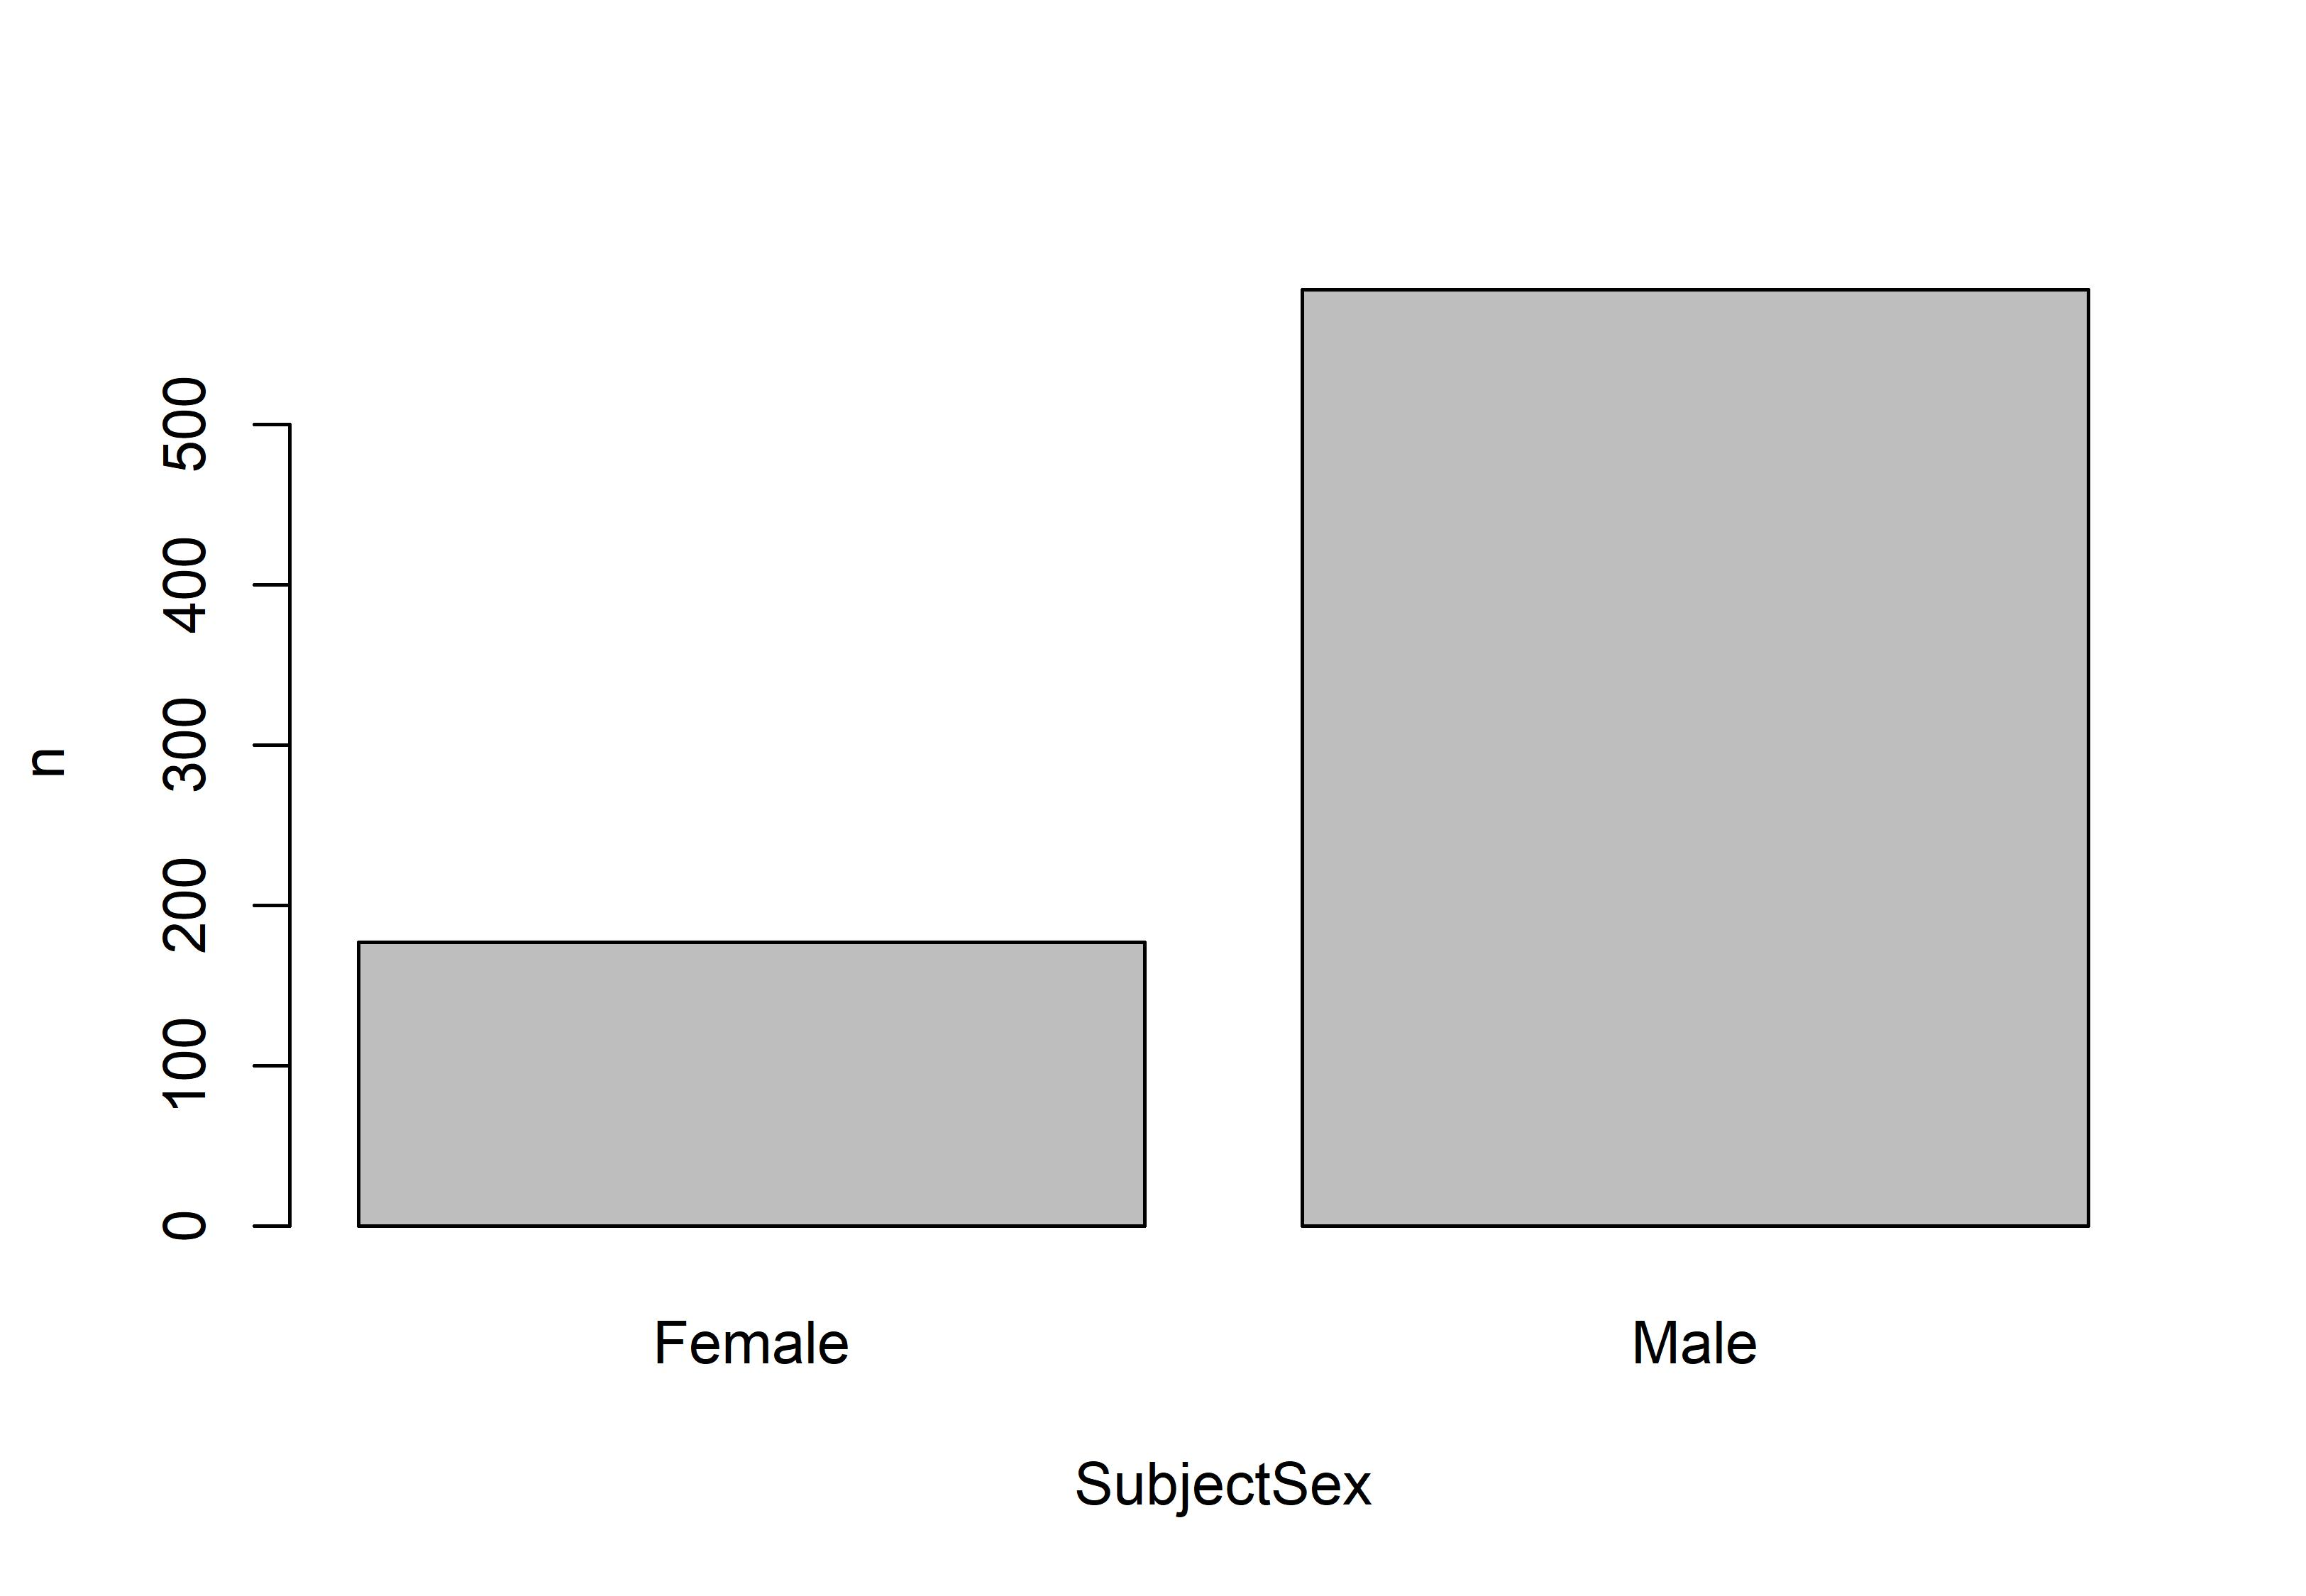
\includegraphics[width=0.4\linewidth]{SurvivR_files/figure-latex/bargraph-1} \end{center}

\begin{Shaded}
\begin{Highlighting}[]

  \FunctionTok{barplot}\NormalTok{(Percent }\SpecialCharTok{\textasciitilde{}}\NormalTok{ SubjectSex, Tab)}
\end{Highlighting}
\end{Shaded}

\begin{center}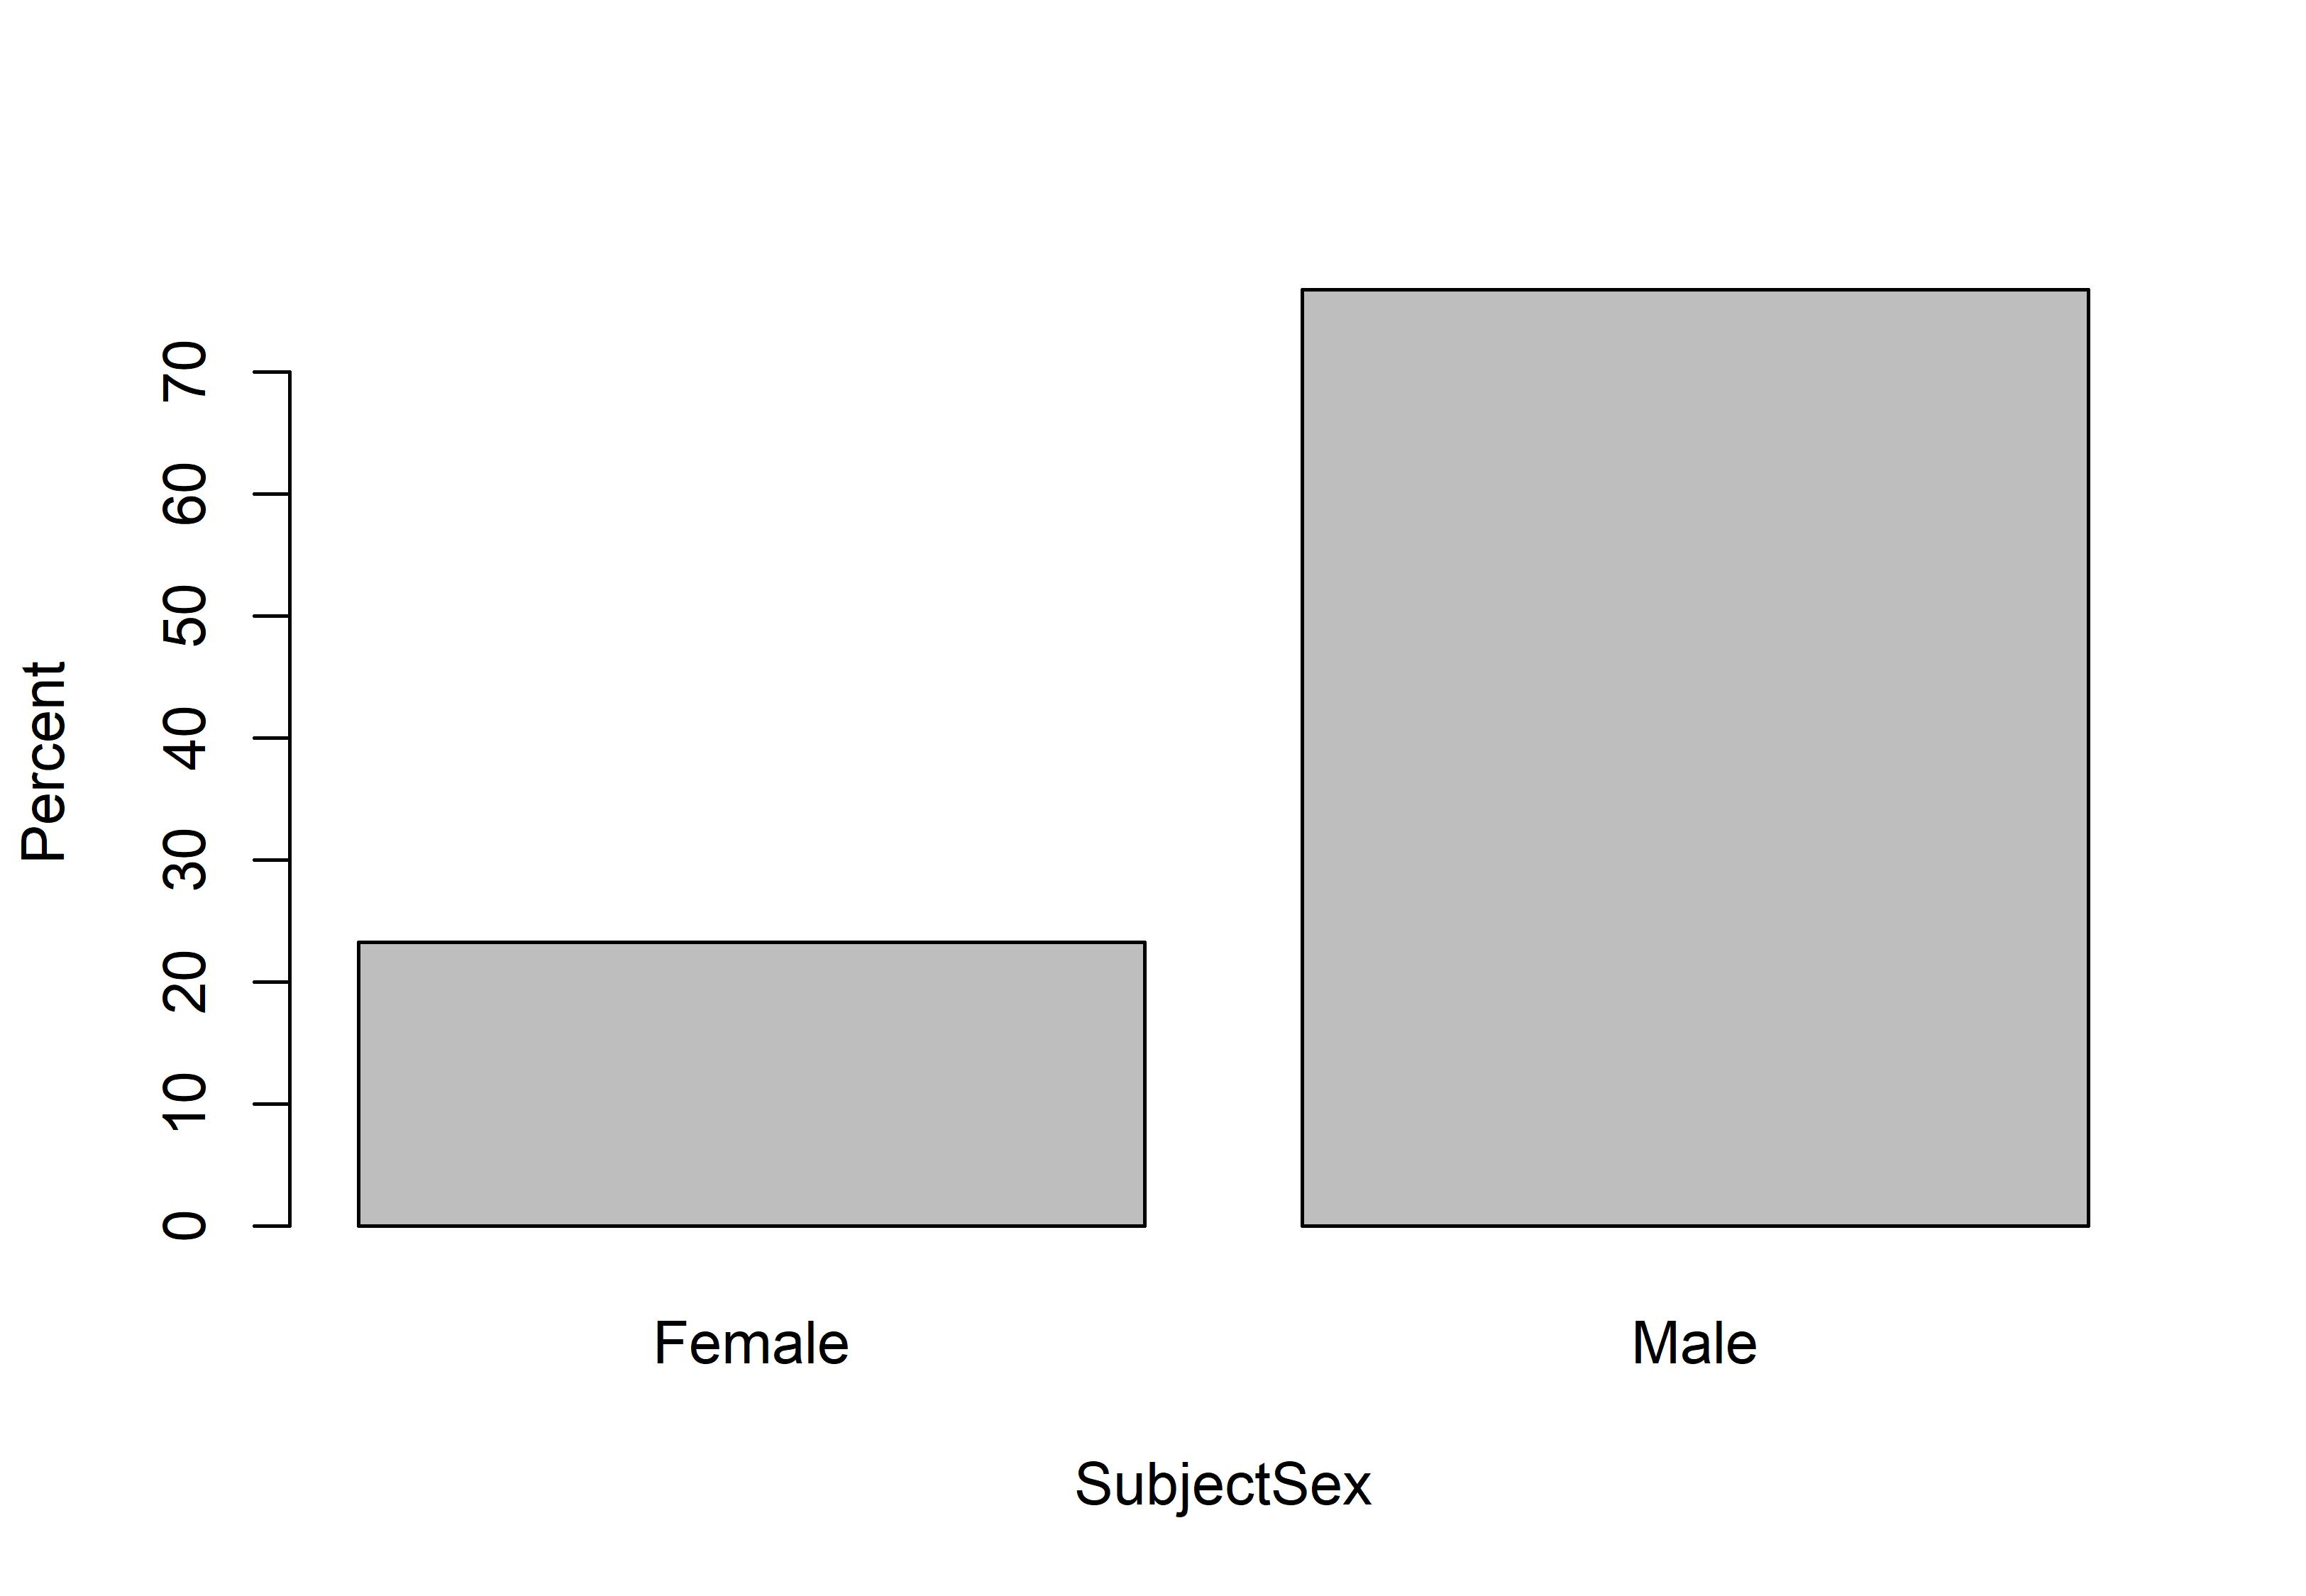
\includegraphics[width=0.4\linewidth]{SurvivR_files/figure-latex/bargraph-2} \end{center}

\hypertarget{cross-tabulation}{%
\section{Cross-tabulation}\label{cross-tabulation}}

There is a three-step process for presenting and evaluating the association between two nominal variables. The first step is to create a basic cross-tabulation of the joint frequency using the \texttt{count()} function. Here we consider the possibility that the representation of female subjects in biopics (\texttt{SubjectSex}) has changed over time (\texttt{Period}).

\begin{Shaded}
\begin{Highlighting}[]
\CommentTok{\# Raw cross{-}tabulation}
\NormalTok{  xtab }\OtherTok{=}
\NormalTok{    film }\SpecialCharTok{\%\textgreater{}\%} 
    \FunctionTok{count}\NormalTok{(SubjectSex,Period) }\SpecialCharTok{\%\textgreater{}\%}  \CommentTok{\# (OutcomeVar,ExposureVar)}
    \FunctionTok{na.omit}\NormalTok{() }\SpecialCharTok{\%\textgreater{}\%} \CommentTok{\# drop NA categories}
  \CommentTok{\# now organize results into a 2{-}way table}
    \FunctionTok{pivot\_wider}\NormalTok{(}
      \AttributeTok{names\_from =}\NormalTok{ Period, }\CommentTok{\# MUST be the ExposureVar}
      \AttributeTok{values\_from =}\NormalTok{ n, }
      \AttributeTok{values\_fill =} \DecValTok{0}
\NormalTok{    )}

\NormalTok{  xtab}
\DocumentationTok{\#\# \# A tibble: 2 x 4}
\DocumentationTok{\#\#   SubjectSex \textasciigrave{}1915{-}{-}1965\textasciigrave{} \textasciigrave{}1965{-}{-}1999\textasciigrave{} \textasciigrave{}2000{-}{-}2014\textasciigrave{}}
\DocumentationTok{\#\#   \textless{}chr\textgreater{}             \textless{}int\textgreater{}        \textless{}int\textgreater{}        \textless{}int\textgreater{}}
\DocumentationTok{\#\# 1 Female               44           59           74}
\DocumentationTok{\#\# 2 Male                132          203          249}
\end{Highlighting}
\end{Shaded}

Use \texttt{chisq.test()} to conduct a \(\chi^2\) test of independence. Specify the contingency table created above and add \texttt{{[}-1{]}} to exclude the first column (category names) from the calculation/

\begin{Shaded}
\begin{Highlighting}[]
  \FunctionTok{chisq.test}\NormalTok{(xtab[}\SpecialCharTok{{-}}\DecValTok{1}\NormalTok{])}
\end{Highlighting}
\end{Shaded}

\begin{verbatim}
## 
##  Pearson's Chi-squared test
## 
## data:  xtab[-1]
## X-squared = 0.4, df = 2, p-value = 0.8
\end{verbatim}

Based on these results, the given sex of biopic subjects is independent of (ie does not differ systematically across) time period. The relationship is not statistically significant (\(\chi^2(2,N=761)=0.40\), \(p=0.81\)).

To present and interpret the results of a cross-tabulation, convert the raw frequencies in each cell to the relative frequency (within categories of the the exposure variable). Start by calling the raw tabulation from above.

\begin{Shaded}
\begin{Highlighting}[]
\CommentTok{\# Relative freq for presentations  }
\NormalTok{  xtab }\SpecialCharTok{\%\textgreater{}\%}
  \CommentTok{\# add a row total}
    \FunctionTok{mutate}\NormalTok{(}\AttributeTok{Total =} \FunctionTok{rowSums}\NormalTok{(.[}\SpecialCharTok{{-}}\DecValTok{1}\NormalTok{])) }\SpecialCharTok{\%\textgreater{}\%}
  \CommentTok{\# convert to percentage}
    \FunctionTok{mutate\_at}\NormalTok{(}\SpecialCharTok{{-}}\DecValTok{1}\NormalTok{, }\SpecialCharTok{\textasciitilde{}} \FunctionTok{round}\NormalTok{(}\DecValTok{100} \SpecialCharTok{*}\NormalTok{ .}\SpecialCharTok{/}\FunctionTok{sum}\NormalTok{(.), }\AttributeTok{digits=}\DecValTok{1}\NormalTok{))}
\end{Highlighting}
\end{Shaded}

\begin{verbatim}
## # A tibble: 2 x 5
##   SubjectSex `1915--1965` `1965--1999` `2000--2014`
##   <chr>             <dbl>        <dbl>        <dbl>
## 1 Female               25         22.5         22.9
## 2 Male                 75         77.5         77.1
## # ... with 1 more variable: Total <dbl>
\end{verbatim}

Copy and paste the table into your document. Then format appropriately (e.g.~category labels) for final presentation.

\hypertarget{regression-analysis}{%
\chapter{Regression analysis}\label{regression-analysis}}

Regression is a powerful tool for estimating the relationship between an outcome (or dependent) variable and one or more exposure (or independent) variables. Here we cover how to estimate and present regression models in \texttt{R}.

Note that you will need the \texttt{dcps} (\texttt{"DCPS\ testing.RData"}) dataset to replicate the output in this chapter.

\hypertarget{correlation}{%
\section{Correlation}\label{correlation}}

To calculate the correlation coefficient (\texttt{r}) between two numeric variables, use the \texttt{cor.test()} function and specify the model as \texttt{\textasciitilde{}\ Var1\ +\ Var2}. This structure is unusual in that both variables follow the \texttt{\textasciitilde{}}, and the \texttt{+} separates the two.

\begin{Shaded}
\begin{Highlighting}[]
  \FunctionTok{cor.test}\NormalTok{(}\SpecialCharTok{\textasciitilde{}}\NormalTok{ ProfMath }\SpecialCharTok{+}\NormalTok{ ProfLang, dcps)}
\DocumentationTok{\#\# }
\DocumentationTok{\#\#  Pearson\textquotesingle{}s product{-}moment correlation}
\DocumentationTok{\#\# }
\DocumentationTok{\#\# data:  ProfMath and ProfLang}
\DocumentationTok{\#\# t = 22, df = 106, p{-}value \textless{}2e{-}16}
\DocumentationTok{\#\# alternative hypothesis: true correlation is not equal to 0}
\DocumentationTok{\#\# 95 percent confidence interval:}
\DocumentationTok{\#\#  0.8691 0.9369}
\DocumentationTok{\#\# sample estimates:}
\DocumentationTok{\#\#    cor }
\DocumentationTok{\#\# 0.9088}
\end{Highlighting}
\end{Shaded}

Perhaps not surprisingly, the results suggest that math and language proficiency are positively and strongly correlated (\(r=0.91\)). It is unlikely we observe this association by chance alone (\(t=22.4\), \(p<0.001\)).

Use a scatterplot (\texttt{plot()}) to visualize this bivariate association. Be sure to specify the formula as \texttt{OutcomeVar\ \textasciitilde{}\ ExposureVar}:

\begin{Shaded}
\begin{Highlighting}[]
  \FunctionTok{plot}\NormalTok{(ProfMath }\SpecialCharTok{\textasciitilde{}}\NormalTok{ ProfLang, dcps)}
\end{Highlighting}
\end{Shaded}

\begin{center}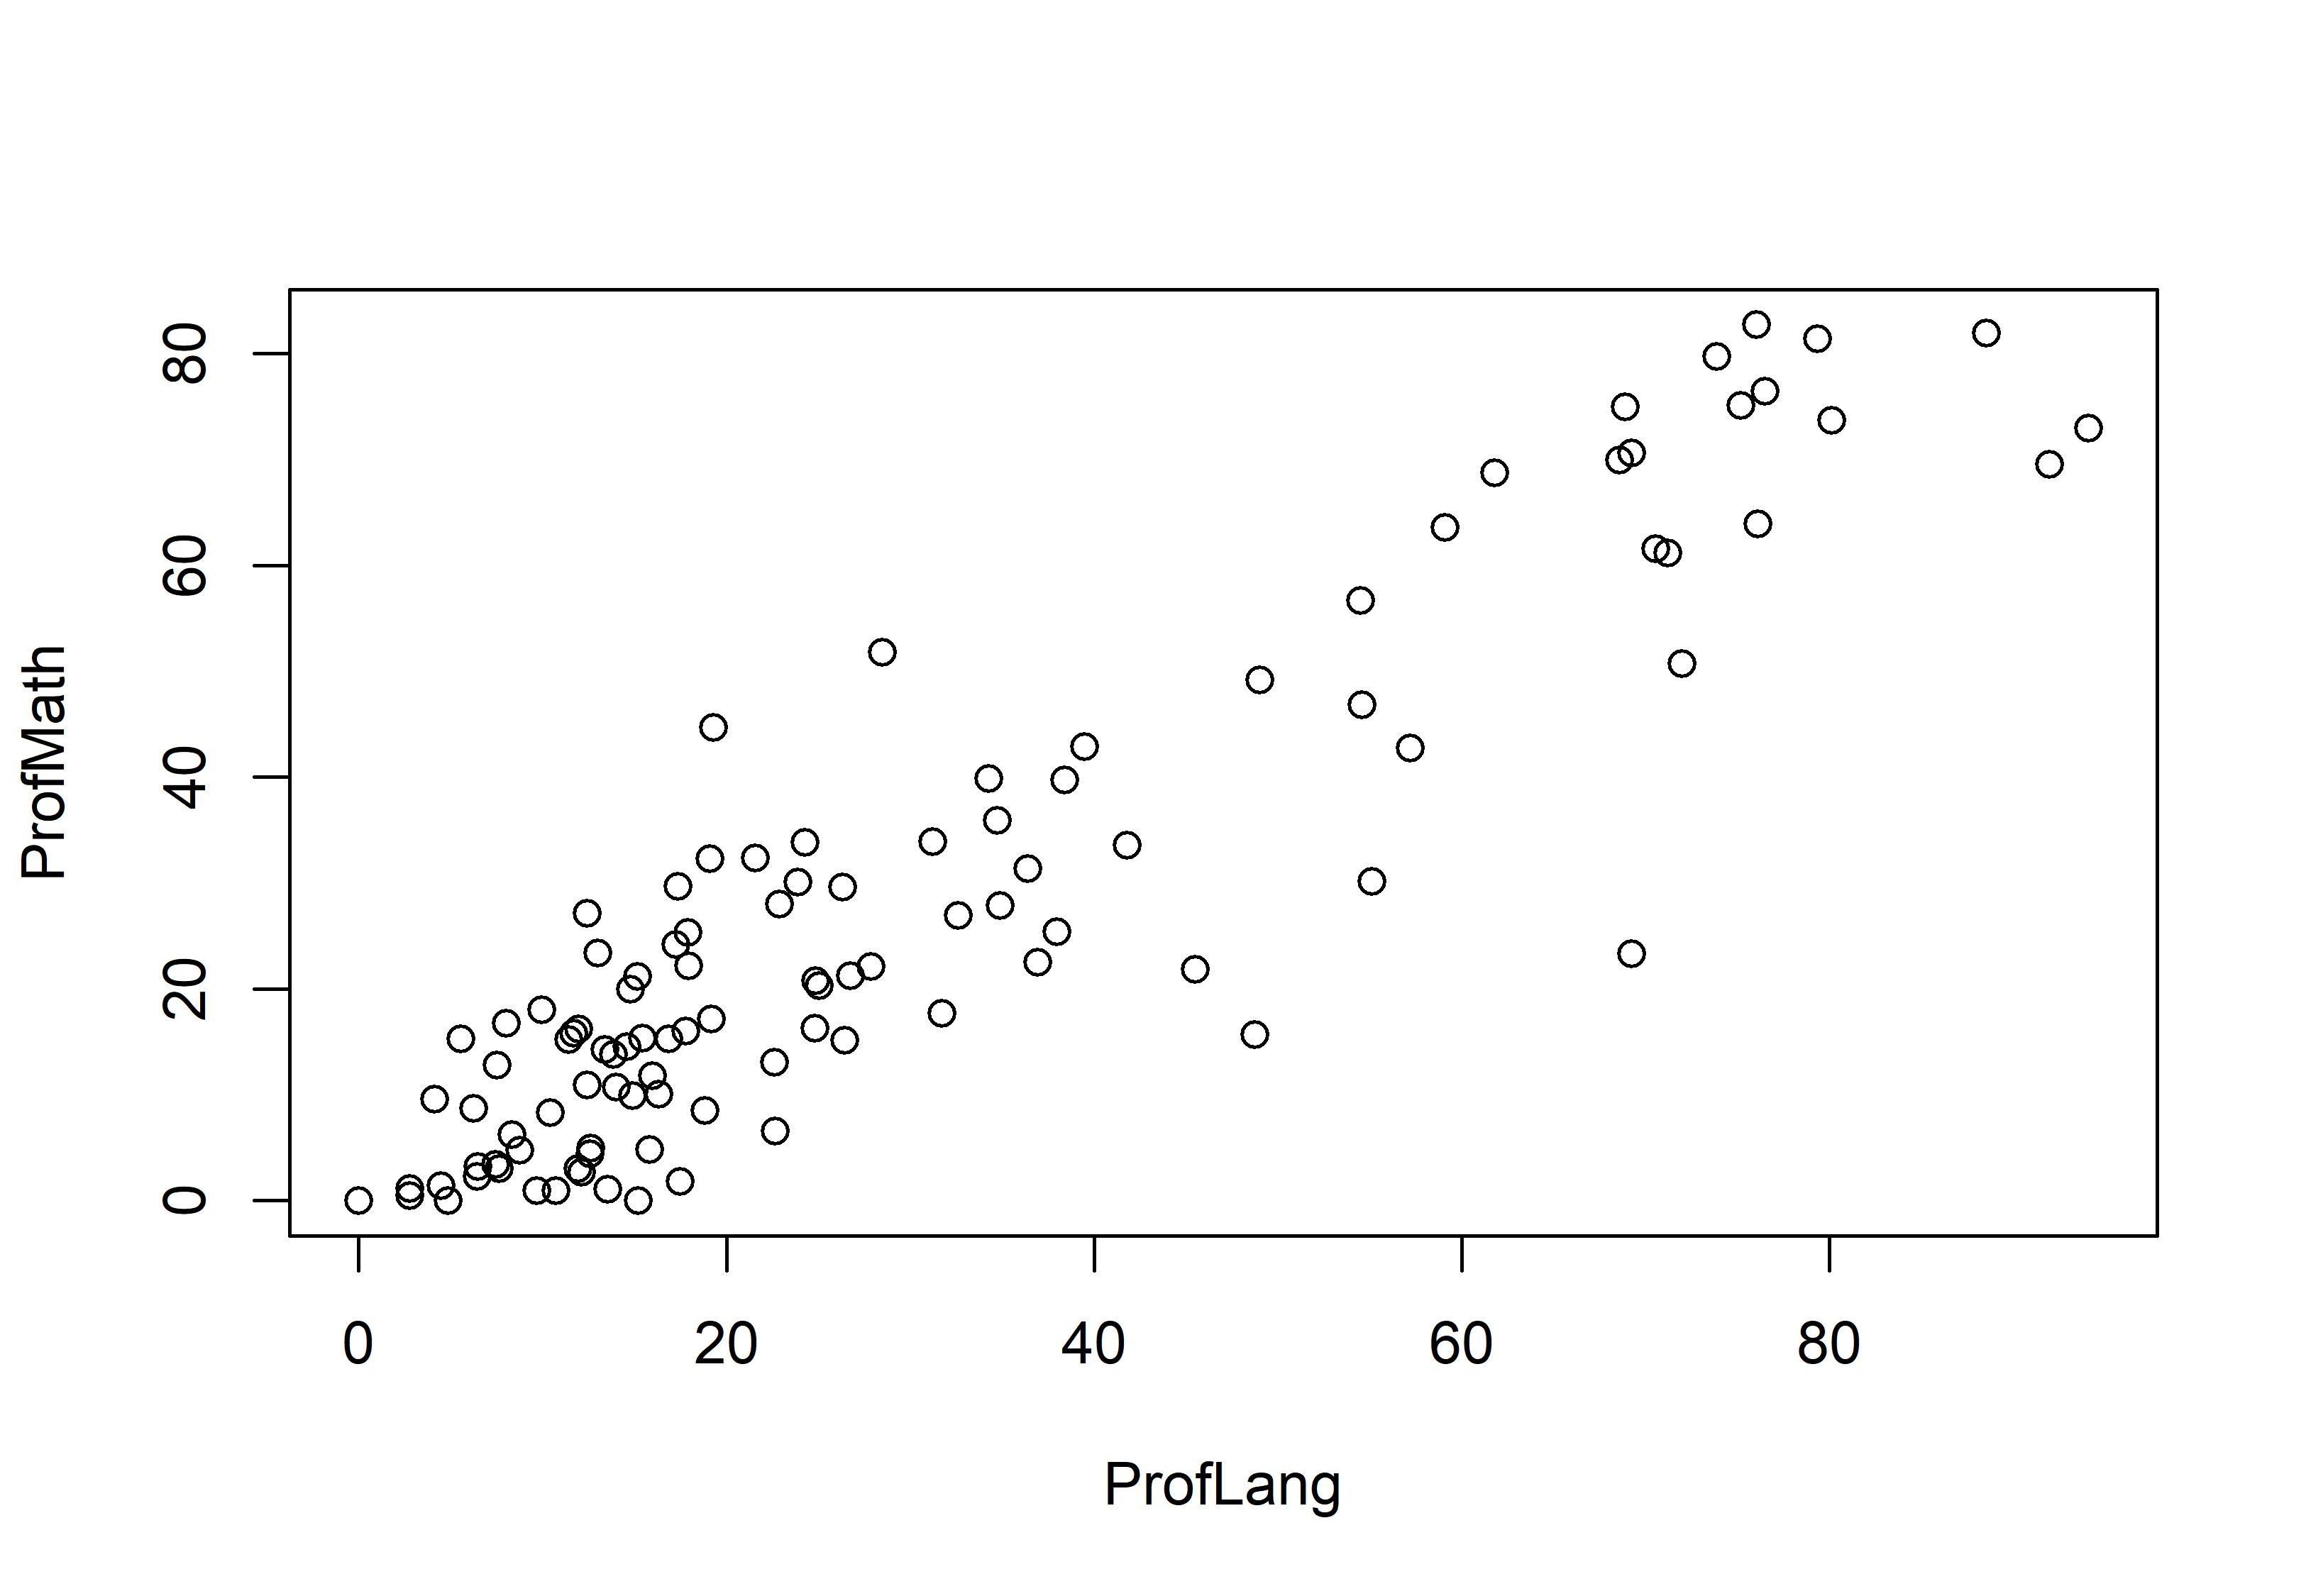
\includegraphics[width=0.4\linewidth]{SurvivR_files/figure-latex/fits-1} \end{center}

\hypertarget{linear-ols-regression}{%
\section{Linear (OLS) regression}\label{linear-ols-regression}}

Estimating a regression equation is simple in R. Using the \texttt{lm()} function will estimate a model with one or more independent variables. Simply specify the formula using the syntax: \texttt{Y\ \textasciitilde{}\ X1\ +\ X2}.

\begin{Shaded}
\begin{Highlighting}[]
\CommentTok{\# Bivariate (unconditional) estimate}
\NormalTok{  Model1 }\OtherTok{\textless{}{-}} \FunctionTok{lm}\NormalTok{(ProfMath }\SpecialCharTok{\textasciitilde{}}\NormalTok{ ProfLang, }\AttributeTok{data =}\NormalTok{ dcps)}

\CommentTok{\# Multivariate (conditional) estimate}
\NormalTok{  Model2 }\OtherTok{\textless{}{-}} \FunctionTok{lm}\NormalTok{(ProfMath }\SpecialCharTok{\textasciitilde{}}\NormalTok{ ProfLang }\SpecialCharTok{+}\NormalTok{ NumTested, }\AttributeTok{data =}\NormalTok{ dcps)}
\end{Highlighting}
\end{Shaded}

To view the coefficient estimates and evaluate hypotheses about the relationship, apply the \texttt{summary()} function to the model object.

\begin{Shaded}
\begin{Highlighting}[]
  \FunctionTok{summary}\NormalTok{(Model1)}
\DocumentationTok{\#\# }
\DocumentationTok{\#\# Call:}
\DocumentationTok{\#\# lm(formula = ProfMath \textasciitilde{} ProfLang, data = dcps)}
\DocumentationTok{\#\# }
\DocumentationTok{\#\# Residuals:}
\DocumentationTok{\#\#    Min     1Q Median     3Q    Max }
\DocumentationTok{\#\# {-}38.23  {-}5.15  {-}0.91   7.17  26.92 }
\DocumentationTok{\#\# }
\DocumentationTok{\#\# Coefficients:}
\DocumentationTok{\#\#             Estimate Std. Error t value Pr(\textgreater{}|t|)    }
\DocumentationTok{\#\# (Intercept)   0.9096     1.5049     0.6     0.55    }
\DocumentationTok{\#\# ProfLang      0.8761     0.0391    22.4   \textless{}2e{-}16 ***}
\DocumentationTok{\#\# {-}{-}{-}}
\DocumentationTok{\#\# Signif. codes:  }
\DocumentationTok{\#\# 0 \textquotesingle{}***\textquotesingle{} 0.001 \textquotesingle{}**\textquotesingle{} 0.01 \textquotesingle{}*\textquotesingle{} 0.05 \textquotesingle{}.\textquotesingle{} 0.1 \textquotesingle{} \textquotesingle{} 1}
\DocumentationTok{\#\# }
\DocumentationTok{\#\# Residual standard error: 9.94 on 106 degrees of freedom}
\DocumentationTok{\#\# Multiple R{-}squared:  0.826,  Adjusted R{-}squared:  0.824 }
\DocumentationTok{\#\# F{-}statistic:  503 on 1 and 106 DF,  p{-}value: \textless{}2e{-}16}

  \FunctionTok{summary}\NormalTok{(Model2)}
\DocumentationTok{\#\# }
\DocumentationTok{\#\# Call:}
\DocumentationTok{\#\# lm(formula = ProfMath \textasciitilde{} ProfLang + NumTested, data = dcps)}
\DocumentationTok{\#\# }
\DocumentationTok{\#\# Residuals:}
\DocumentationTok{\#\#    Min     1Q Median     3Q    Max }
\DocumentationTok{\#\# {-}39.33  {-}5.41  {-}0.80   6.98  26.43 }
\DocumentationTok{\#\# }
\DocumentationTok{\#\# Coefficients:}
\DocumentationTok{\#\#             Estimate Std. Error t value Pr(\textgreater{}|t|)    }
\DocumentationTok{\#\# (Intercept)   2.2109     1.7146    1.29     0.20    }
\DocumentationTok{\#\# ProfLang      0.8943     0.0405   22.06   \textless{}2e{-}16 ***}
\DocumentationTok{\#\# NumTested    {-}0.0102     0.0066   {-}1.55     0.12    }
\DocumentationTok{\#\# {-}{-}{-}}
\DocumentationTok{\#\# Signif. codes:  }
\DocumentationTok{\#\# 0 \textquotesingle{}***\textquotesingle{} 0.001 \textquotesingle{}**\textquotesingle{} 0.01 \textquotesingle{}*\textquotesingle{} 0.05 \textquotesingle{}.\textquotesingle{} 0.1 \textquotesingle{} \textquotesingle{} 1}
\DocumentationTok{\#\# }
\DocumentationTok{\#\# Residual standard error: 9.88 on 105 degrees of freedom}
\DocumentationTok{\#\# Multiple R{-}squared:  0.83,   Adjusted R{-}squared:  0.827 }
\DocumentationTok{\#\# F{-}statistic:  256 on 2 and 105 DF,  p{-}value: \textless{}2e{-}16}
\end{Highlighting}
\end{Shaded}

Notice in each that the independent variables define the rows. In \texttt{Model2}, the estimated slope coefficient for \texttt{ProfLang} is 0.89 with a p-value less than 0.001. This means that on average and net of the number of students tested, a 1-percentage-point increase in language proficiency is associated with a 0.89-percentage-point increase in math proficiency. The association is statistically significant (\(p<0.001\)). We might also note that the variables in the model account for almost 90\% of observed variation in math proficiency across DC Public Schools (\(Adj~R^2=0.83\)).

\hypertarget{scatter-with-linear-fit}{%
\section{Scatter with linear fit}\label{scatter-with-linear-fit}}

We use a scatter plot with linear fit to visualize the bivariate (unconditional) linear associations. First create the scatter with \texttt{plot()} and then overlay the regression line from stored estimates using \texttt{abline()}. Be sure to run these lines together or in succession:

\begin{Shaded}
\begin{Highlighting}[]
  \CommentTok{\# Plot the scatter}
    \FunctionTok{plot}\NormalTok{(ProfMath }\SpecialCharTok{\textasciitilde{}}\NormalTok{ ProfLang, dcps)}

  \CommentTok{\# Add stored linear estimate}
    \FunctionTok{abline}\NormalTok{(Model1)}
\end{Highlighting}
\end{Shaded}

\begin{center}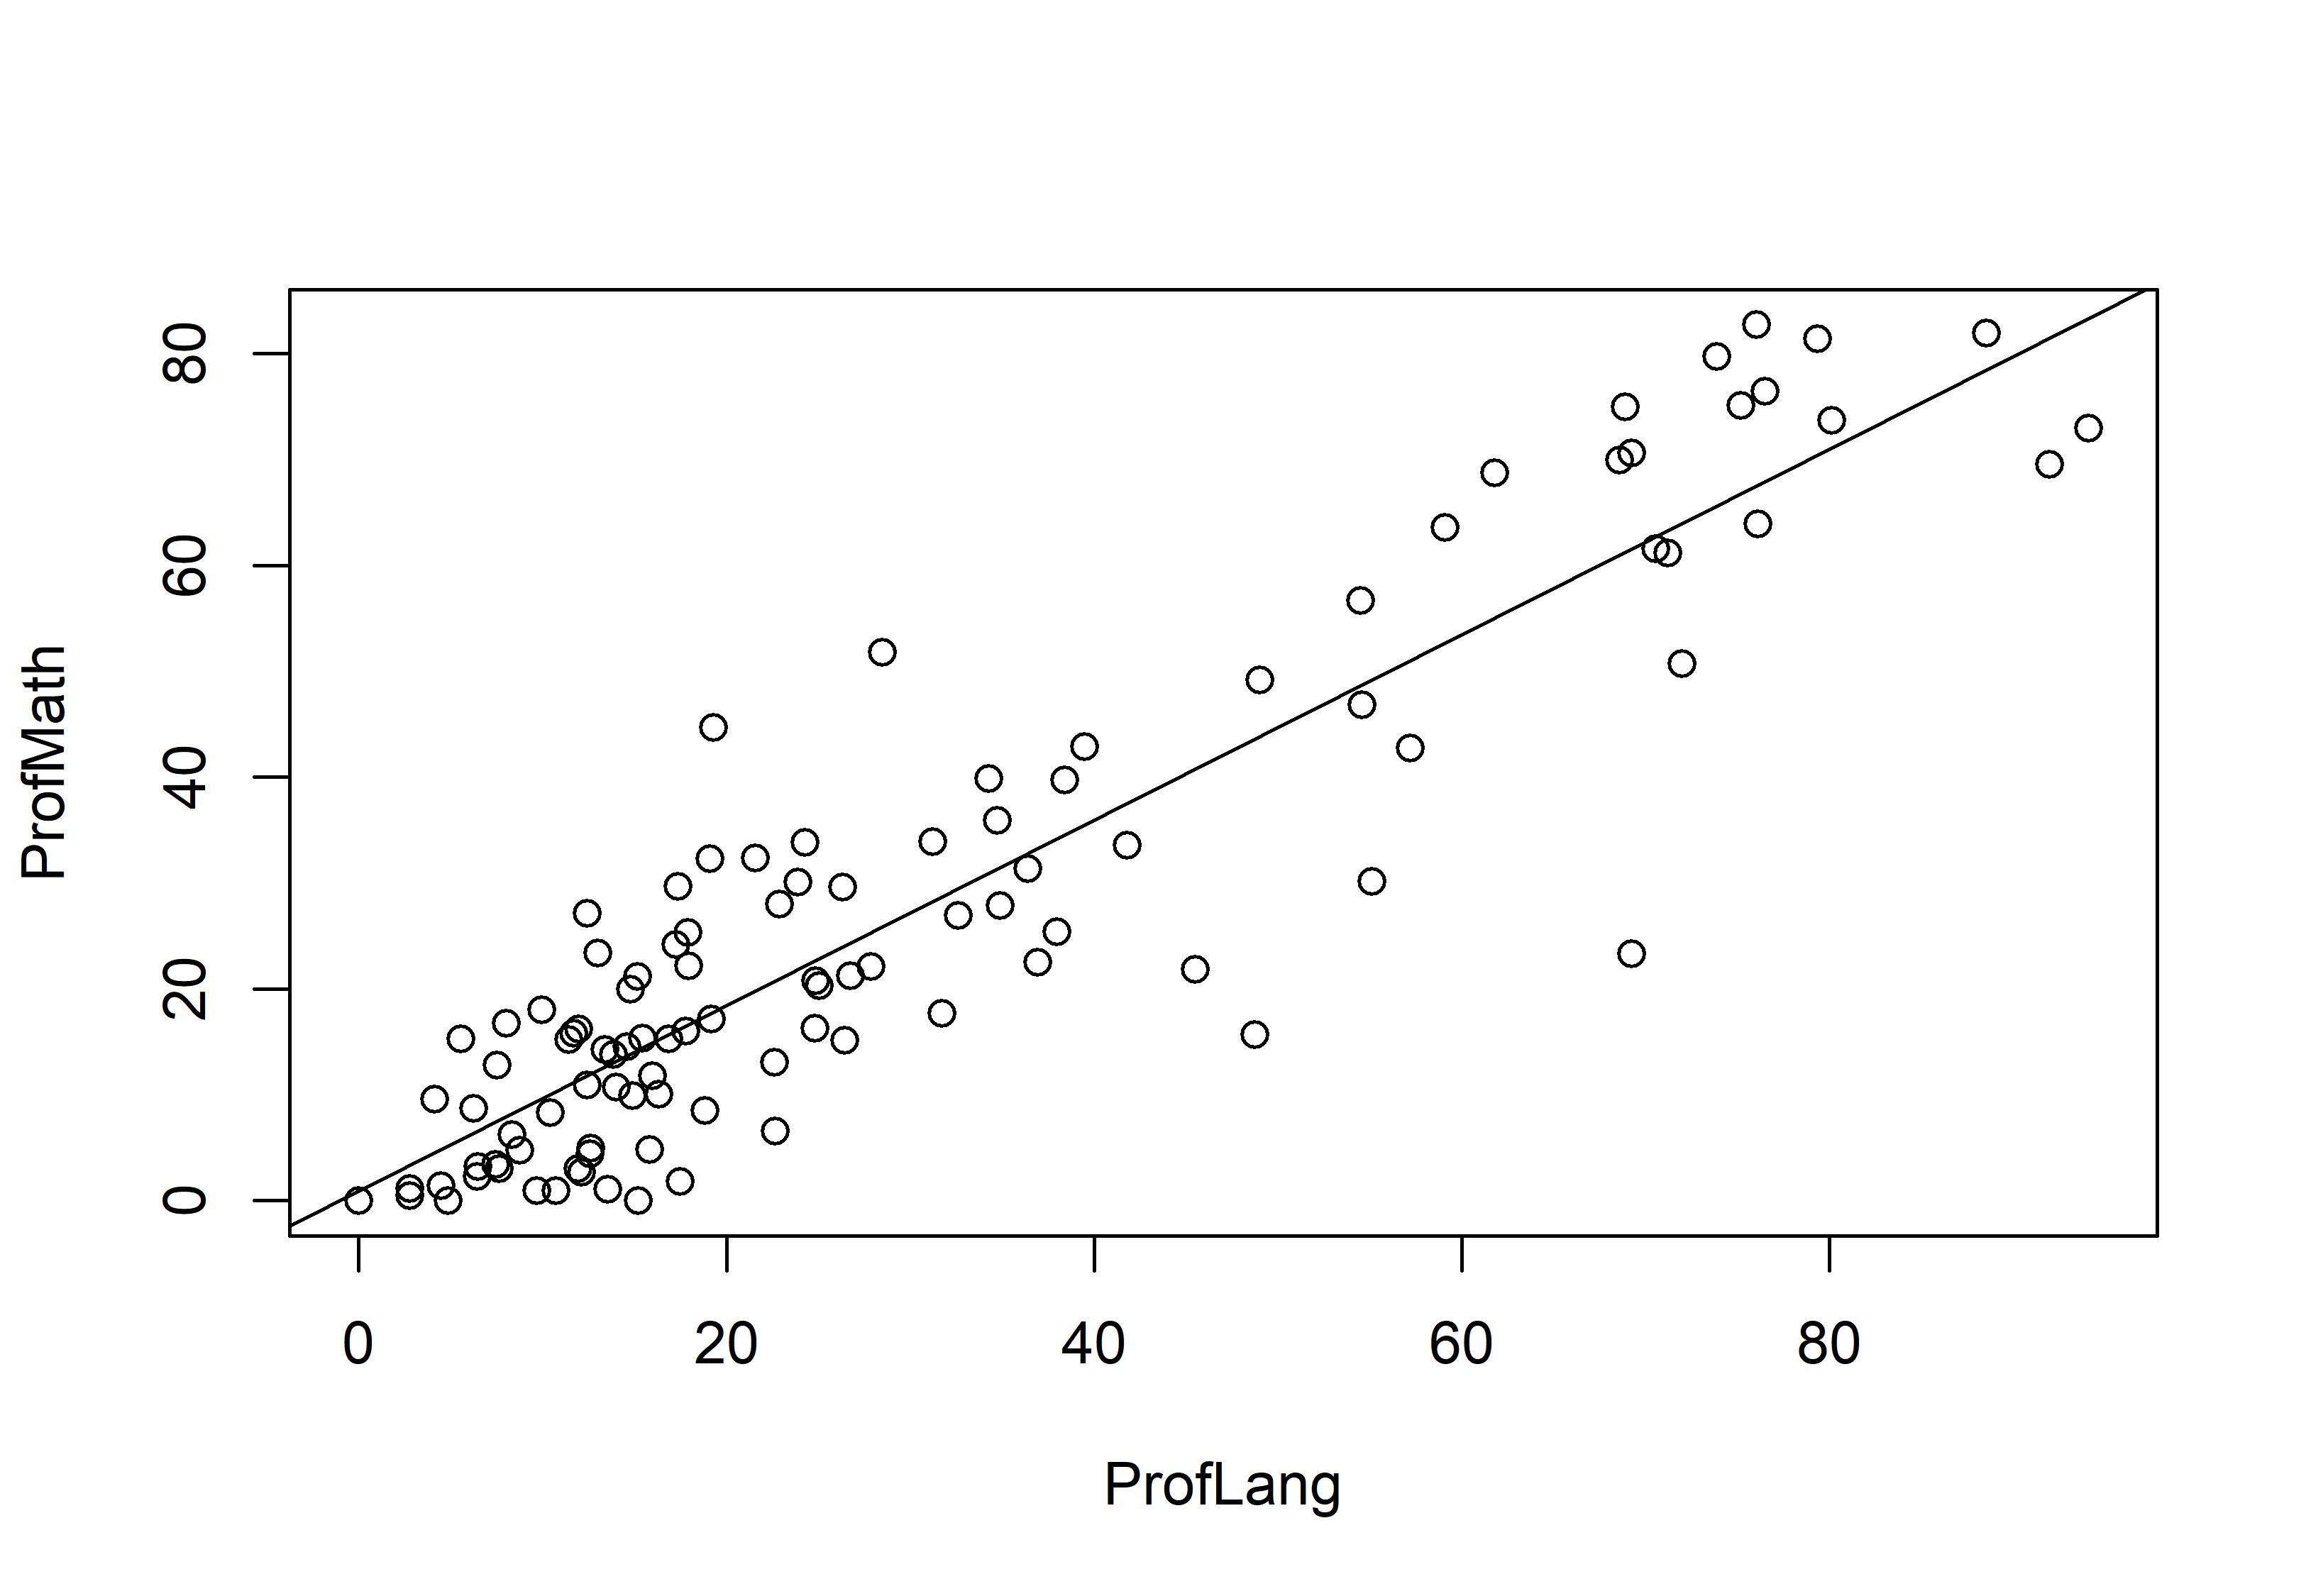
\includegraphics[width=0.4\linewidth]{SurvivR_files/figure-latex/fits2-1} \end{center}

\hypertarget{logistic-regression}{%
\section{Logistic regression}\label{logistic-regression}}

With a binary outcome measure, logistic regression is generally more appropriate than linear (OLS) regression. Use the \texttt{glm()} function to estimate a generalized model, and specify the model family as \texttt{binomial} within the arguments.

\begin{Shaded}
\begin{Highlighting}[]
\CommentTok{\# create binary measure of "above average math proficiency"}
\NormalTok{  dcps }\OtherTok{=}
\NormalTok{    dcps }\SpecialCharTok{\%\textgreater{}\%}
    \FunctionTok{mutate}\NormalTok{(}\AttributeTok{AboveAvgMath =} \FunctionTok{if\_else}\NormalTok{(ProfMath }\SpecialCharTok{\textgreater{}} \FunctionTok{mean}\NormalTok{(ProfMath),}\DecValTok{1}\NormalTok{,}\DecValTok{0}\NormalTok{))}

\NormalTok{  Model3 }\OtherTok{=} 
    \FunctionTok{glm}\NormalTok{(}
\NormalTok{      AboveAvgMath }\SpecialCharTok{\textasciitilde{}}\NormalTok{ ProfLang }\SpecialCharTok{+}\NormalTok{ NumTested,  }\CommentTok{\# specify model}
      \AttributeTok{family =} \StringTok{\textquotesingle{}binomial\textquotesingle{}}\NormalTok{,  }\CommentTok{\# logistic estimation}
      \AttributeTok{data =}\NormalTok{ dcps}
\NormalTok{    )}
\end{Highlighting}
\end{Shaded}

To view the coefficient estimates and evaluate hypotheses, again apply the \texttt{summary()} function to the model object.

\begin{Shaded}
\begin{Highlighting}[]
\CommentTok{\# View estimates}
  \FunctionTok{summary}\NormalTok{(Model3)  }
\DocumentationTok{\#\# }
\DocumentationTok{\#\# Call:}
\DocumentationTok{\#\# glm(formula = AboveAvgMath \textasciitilde{} ProfLang + NumTested, family = "binomial", }
\DocumentationTok{\#\#     data = dcps)}
\DocumentationTok{\#\# }
\DocumentationTok{\#\# Deviance Residuals: }
\DocumentationTok{\#\#    Min      1Q  Median      3Q     Max  }
\DocumentationTok{\#\# {-}2.938  {-}0.547  {-}0.351   0.213   2.115  }
\DocumentationTok{\#\# }
\DocumentationTok{\#\# Coefficients:}
\DocumentationTok{\#\#             Estimate Std. Error z value Pr(\textgreater{}|z|)    }
\DocumentationTok{\#\# (Intercept) {-}3.22427    0.61253   {-}5.26  1.4e{-}07 ***}
\DocumentationTok{\#\# ProfLang     0.11366    0.02412    4.71  2.4e{-}06 ***}
\DocumentationTok{\#\# NumTested   {-}0.00239    0.00229   {-}1.04      0.3    }
\DocumentationTok{\#\# {-}{-}{-}}
\DocumentationTok{\#\# Signif. codes:  }
\DocumentationTok{\#\# 0 \textquotesingle{}***\textquotesingle{} 0.001 \textquotesingle{}**\textquotesingle{} 0.01 \textquotesingle{}*\textquotesingle{} 0.05 \textquotesingle{}.\textquotesingle{} 0.1 \textquotesingle{} \textquotesingle{} 1}
\DocumentationTok{\#\# }
\DocumentationTok{\#\# (Dispersion parameter for binomial family taken to be 1)}
\DocumentationTok{\#\# }
\DocumentationTok{\#\#     Null deviance: 144.342  on 107  degrees of freedom}
\DocumentationTok{\#\# Residual deviance:  77.127  on 105  degrees of freedom}
\DocumentationTok{\#\# AIC: 83.13}
\DocumentationTok{\#\# }
\DocumentationTok{\#\# Number of Fisher Scoring iterations: 6}

\CommentTok{\# Odds ratios}
  \FunctionTok{exp}\NormalTok{(}\FunctionTok{coef}\NormalTok{(Model3))}
\DocumentationTok{\#\# (Intercept)    ProfLang   NumTested }
\DocumentationTok{\#\#     0.03978     1.12037     0.99761}
\end{Highlighting}
\end{Shaded}

The results indicate that a percentage-point increase in a school's language proficiency is expected to raise the odds of being above average in math by 12\%, conditional on the number of students tested. Again, the increase is significant (\(p < 0.001\)).

\hypertarget{making-regression-tables}{%
\section{Making regression tables}\label{making-regression-tables}}

Use the \texttt{stargazer()} function to transform messy \texttt{R} regression estimates into professional and exportable regression tables. Be sure you have installed and loaded the \texttt{stargazer} package. Then simply specify the model estimates to include.

\begin{Shaded}
\begin{Highlighting}[]
  \FunctionTok{library}\NormalTok{(stargazer)}
  
  \FunctionTok{stargazer}\NormalTok{(}
\NormalTok{   Model1, Model2,    }\CommentTok{\# stored estimates to include in the table}
   \AttributeTok{type =} \StringTok{\textquotesingle{}text\textquotesingle{}}\NormalTok{,    }
   \AttributeTok{keep.stat =} \StringTok{\textquotesingle{}n\textquotesingle{}}   \CommentTok{\# add \#obs from each model}
\NormalTok{  ) }
\DocumentationTok{\#\# }
\DocumentationTok{\#\# =========================================}
\DocumentationTok{\#\#                  Dependent variable:     }
\DocumentationTok{\#\#              {-}{-}{-}{-}{-}{-}{-}{-}{-}{-}{-}{-}{-}{-}{-}{-}{-}{-}{-}{-}{-}{-}{-}{-}{-}{-}{-}{-}}
\DocumentationTok{\#\#                        ProfMath          }
\DocumentationTok{\#\#                   (1)            (2)     }
\DocumentationTok{\#\# {-}{-}{-}{-}{-}{-}{-}{-}{-}{-}{-}{-}{-}{-}{-}{-}{-}{-}{-}{-}{-}{-}{-}{-}{-}{-}{-}{-}{-}{-}{-}{-}{-}{-}{-}{-}{-}{-}{-}{-}{-}}
\DocumentationTok{\#\# ProfLang        0.876***      0.894***   }
\DocumentationTok{\#\#                 (0.039)        (0.041)   }
\DocumentationTok{\#\#                                          }
\DocumentationTok{\#\# NumTested                      {-}0.010    }
\DocumentationTok{\#\#                                (0.007)   }
\DocumentationTok{\#\#                                          }
\DocumentationTok{\#\# Constant         0.910          2.211    }
\DocumentationTok{\#\#                 (1.505)        (1.715)   }
\DocumentationTok{\#\#                                          }
\DocumentationTok{\#\# {-}{-}{-}{-}{-}{-}{-}{-}{-}{-}{-}{-}{-}{-}{-}{-}{-}{-}{-}{-}{-}{-}{-}{-}{-}{-}{-}{-}{-}{-}{-}{-}{-}{-}{-}{-}{-}{-}{-}{-}{-}}
\DocumentationTok{\#\# Observations      108            108     }
\DocumentationTok{\#\# =========================================}
\DocumentationTok{\#\# Note:         *p\textless{}0.1; **p\textless{}0.05; ***p\textless{}0.01}
\end{Highlighting}
\end{Shaded}

You can copy and paste these into a program like Excel or Word, and have a nice table with only a few edits.

\hypertarget{doing-more-with-data-frames}{%
\chapter{Doing more with data frames}\label{doing-more-with-data-frames}}

Very few data sets come ``ready-made'' for analysis. Even in our introductory course, there are times when you will need to limit your analysis to certain observations, recode a variable, and more. This chapter covers a few basics of data ``munging.''

Note that you will need the \texttt{film} (\texttt{"biopics.xls"}) and \texttt{dcps} (\texttt{"DCPS\ testing.RData"}) datasets to replicate the commands.

\hypertarget{filtersubset-data}{%
\section{Filter/subset data}\label{filtersubset-data}}

It is often necessary to limit your analysis to some subset of cases. Use the \texttt{filter()} command to specify the criteria by which to select cases.

\begin{Shaded}
\begin{Highlighting}[]
\NormalTok{  film }\OtherTok{=}
\NormalTok{    film }\SpecialCharTok{\%\textgreater{}\%}
    \FunctionTok{filter}\NormalTok{(SubjectSex }\SpecialCharTok{==} \StringTok{\textquotesingle{}Female\textquotesingle{}}\NormalTok{) }\CommentTok{\# criteria for keeping cases}

  \FunctionTok{head}\NormalTok{(film)}
\end{Highlighting}
\end{Shaded}

\begin{verbatim}
## # A tibble: 6 x 10
##   Title Release NumSubjects SubjectName SubjectType
##   <chr>   <dbl>       <dbl> <chr>       <chr>      
## 1 Big ~    2014           1 Margaret K~ Artist     
## 2 Test~    2014           1 Vera Britt~ Other      
## 3 The ~    2014           1 Brittany M~ Actress    
## 4 Wild     2014           1 Cheryl Str~ Other      
## 5 Diana    2013           1 Princess D~ Other      
## 6 Love~    2013           1 Linda Love~ Actress    
## # ... with 5 more variables: SubjectRace <chr>,
## #   PersonOfColor <dbl>, SubjectSex <chr>,
## #   LeadActor <chr>, Period <chr>
\end{verbatim}

The conditions inside \texttt{filter()} identify the cases, or rows, to keep (i.e.~you're selecting only those rows that satisfy the given conditions). This can be based on any number of conditions. Note that a double equals sign \texttt{==} is used to check a logical condition.

\hypertarget{selecting-your-variables}{%
\section{Selecting your variables}\label{selecting-your-variables}}

A dataframe with loads of variables can be unwieldy. Use the \texttt{select()} function to isolate the variables you need for your analysis.

\begin{Shaded}
\begin{Highlighting}[]
\NormalTok{  Study1 }\OtherTok{=}
\NormalTok{    film }\SpecialCharTok{\%\textgreater{}\%}
    \FunctionTok{select}\NormalTok{(Title,Release,SubjectSex)}

  \FunctionTok{head}\NormalTok{(Study1)}
\DocumentationTok{\#\# \# A tibble: 6 x 3}
\DocumentationTok{\#\#   Title                     Release SubjectSex}
\DocumentationTok{\#\#   \textless{}chr\textgreater{}                       \textless{}dbl\textgreater{} \textless{}chr\textgreater{}     }
\DocumentationTok{\#\# 1 Big Eyes                     2014 Female    }
\DocumentationTok{\#\# 2 Testament of Youth           2014 Female    }
\DocumentationTok{\#\# 3 The Brittany Murphy Story    2014 Female    }
\DocumentationTok{\#\# 4 Wild                         2014 Female    }
\DocumentationTok{\#\# 5 Diana                        2013 Female    }
\DocumentationTok{\#\# 6 Lovelace                     2013 Female}
\end{Highlighting}
\end{Shaded}

\hypertarget{create-new-variables}{%
\section{Create new variables}\label{create-new-variables}}

The \texttt{mutate()} function creates new variables (or columns) in a data frame. By assigning the same object name to the result, the new variables become part of the object.

\begin{Shaded}
\begin{Highlighting}[]
\NormalTok{  dcps }\OtherTok{=}
\NormalTok{    dcps }\SpecialCharTok{\%\textgreater{}\%}
    \FunctionTok{mutate}\NormalTok{(}
      \AttributeTok{LastEdit =} \StringTok{\textquotesingle{}2021\textquotesingle{}}\NormalTok{,  }\CommentTok{\# character variable with same value in each}
      \AttributeTok{ProfLangProp =}\NormalTok{ ProfLang}\SpecialCharTok{/}\DecValTok{100}\NormalTok{, }\CommentTok{\# convert to proportion}
\NormalTok{    )}
  
\NormalTok{  dcps }\SpecialCharTok{\%\textgreater{}\%} \FunctionTok{select}\NormalTok{(}\DecValTok{2}\NormalTok{,}\DecValTok{5}\NormalTok{,}\DecValTok{8}\SpecialCharTok{:}\DecValTok{9}\NormalTok{) }\SpecialCharTok{\%\textgreater{}\%} \FunctionTok{head}\NormalTok{()}
\DocumentationTok{\#\# \# A tibble: 6 x 4}
\DocumentationTok{\#\#   SchName                ProfLang AboveAvgMath LastEdit}
\DocumentationTok{\#\#   \textless{}chr\textgreater{}                     \textless{}dbl\textgreater{}        \textless{}dbl\textgreater{} \textless{}chr\textgreater{}   }
\DocumentationTok{\#\# 1 Aiton Elementary Scho\textasciitilde{}     5.56            0 2021    }
\DocumentationTok{\#\# 2 Amidon{-}Bowen Elementa\textasciitilde{}    16.3             0 2021    }
\DocumentationTok{\#\# 3 Anacostia High School      4.48            0 2021    }
\DocumentationTok{\#\# 4 Ballou High School         2.78            0 2021    }
\DocumentationTok{\#\# 5 Bancroft Elementary S\textasciitilde{}    34.3             1 2021    }
\DocumentationTok{\#\# 6 Barnard Elementary Sc\textasciitilde{}    38.4             1 2021}
\end{Highlighting}
\end{Shaded}

In addition to transformations that apply the same function to every case, you can create variables that treat cases on an individual basis. Consider the \texttt{if\_else()} option. This will specify a logical test to apply to each case, and specify replacement values for those cases that evaluate as true and those cases that evaluate as false. The syntax is: \texttt{if\_else(criteria,value.if.true,value.if.false)}.

\begin{Shaded}
\begin{Highlighting}[]
\NormalTok{  dcps }\OtherTok{=}
\NormalTok{    dcps }\SpecialCharTok{\%\textgreater{}\%}
    \FunctionTok{mutate}\NormalTok{(}
      \AttributeTok{AbvMedMath =} \FunctionTok{if\_else}\NormalTok{(}
\NormalTok{        ProfMath }\SpecialCharTok{\textgreater{}} \FunctionTok{median}\NormalTok{(ProfMath), }\CommentTok{\# condition to evaluate}
        \DecValTok{1}\NormalTok{,  }\CommentTok{\# output if condition is TRUE}
        \DecValTok{0}   \CommentTok{\# output if FALSE}
\NormalTok{      )}
\NormalTok{    )}

\NormalTok{  dcps }\SpecialCharTok{\%\textgreater{}\%} \FunctionTok{select}\NormalTok{(SchCode,ProfMath,AbvMedMath) }\SpecialCharTok{\%\textgreater{}\%} \FunctionTok{head}\NormalTok{()}
\DocumentationTok{\#\# \# A tibble: 6 x 3}
\DocumentationTok{\#\#   SchCode ProfMath AbvMedMath}
\DocumentationTok{\#\#     \textless{}dbl\textgreater{}    \textless{}dbl\textgreater{}      \textless{}dbl\textgreater{}}
\DocumentationTok{\#\# 1     202   15.3            0}
\DocumentationTok{\#\# 2     203   10.1            0}
\DocumentationTok{\#\# 3     450    1.43           0}
\DocumentationTok{\#\# 4     452    0.498          0}
\DocumentationTok{\#\# 5     204   39.9            1}
\DocumentationTok{\#\# 6     205   39.7            1}
\end{Highlighting}
\end{Shaded}

\hypertarget{appending-and-merging-data}{%
\section{Appending and merging data}\label{appending-and-merging-data}}

It is often useful to combine data from different sources. This may take the form of appending (adding additional cases with information on the same variables) or merging (adding additional variables that describe the same cases).

\hypertarget{appending-new-cases}{%
\subsection{Appending new cases}\label{appending-new-cases}}

To append new cases to your data frame, use \texttt{bind\_rows(OldData,NewData)}. Note that the variable names need to match exactly across data frames, but the variable order does not matter.

\begin{Shaded}
\begin{Highlighting}[]
  \CommentTok{\# old data}
\NormalTok{    myData }\OtherTok{=} \FunctionTok{tribble}\NormalTok{(}
      \SpecialCharTok{\textasciitilde{}}\NormalTok{District, }\SpecialCharTok{\textasciitilde{}}\NormalTok{Students,}
      \DecValTok{115}\NormalTok{, }\DecValTok{985}\NormalTok{,}
      \DecValTok{116}\NormalTok{, }\DecValTok{1132}
\NormalTok{    )}

  \CommentTok{\# new data to add}
\NormalTok{    new }\OtherTok{=} \FunctionTok{tribble}\NormalTok{(}
      \SpecialCharTok{\textasciitilde{}}\NormalTok{District, }\SpecialCharTok{\textasciitilde{}}\NormalTok{Students,}
      \DecValTok{117}\NormalTok{, }\DecValTok{419}\NormalTok{,}
      \DecValTok{118}\NormalTok{, }\DecValTok{633}
\NormalTok{    )}
    
  \CommentTok{\# Append new to old}
\NormalTok{    myData }\OtherTok{=} \FunctionTok{bind\_rows}\NormalTok{(myData,new)}
    
\NormalTok{    myData}
\DocumentationTok{\#\# \# A tibble: 4 x 2}
\DocumentationTok{\#\#   District Students}
\DocumentationTok{\#\#      \textless{}dbl\textgreater{}    \textless{}dbl\textgreater{}}
\DocumentationTok{\#\# 1      115      985}
\DocumentationTok{\#\# 2      116     1132}
\DocumentationTok{\#\# 3      117      419}
\DocumentationTok{\#\# 4      118      633}
\end{Highlighting}
\end{Shaded}

\hypertarget{merging}{%
\subsection{Merging}\label{merging}}

To merge data frames (add new variables for existing cases), use \texttt{left\_join(OldData,NewData)}. In order to link rows in one data frame to rows in another, it is critical that the data sets contain a common identifier, with the same variable name and same values. Building on the example above

\begin{Shaded}
\begin{Highlighting}[]
  \CommentTok{\# new variables}
\NormalTok{    newvars }\OtherTok{=} \FunctionTok{tribble}\NormalTok{(}
      \SpecialCharTok{\textasciitilde{}}\NormalTok{District,}\SpecialCharTok{\textasciitilde{}}\NormalTok{Teachers,}
      \DecValTok{115}\NormalTok{, }\DecValTok{43}\NormalTok{,}
      \DecValTok{116}\NormalTok{, }\DecValTok{71}\NormalTok{,}
      \DecValTok{118}\NormalTok{, }\DecValTok{55}
\NormalTok{    )}

  \CommentTok{\# join new to old}
\NormalTok{    myData }\OtherTok{=} \FunctionTok{left\_join}\NormalTok{(myData,newvars)}
\DocumentationTok{\#\# Joining, by = "District"}
    
\NormalTok{    myData}
\DocumentationTok{\#\# \# A tibble: 4 x 3}
\DocumentationTok{\#\#   District Students Teachers}
\DocumentationTok{\#\#      \textless{}dbl\textgreater{}    \textless{}dbl\textgreater{}    \textless{}dbl\textgreater{}}
\DocumentationTok{\#\# 1      115      985       43}
\DocumentationTok{\#\# 2      116     1132       71}
\DocumentationTok{\#\# 3      117      419       NA}
\DocumentationTok{\#\# 4      118      633       55}
\end{Highlighting}
\end{Shaded}

\hypertarget{basic-visualization}{%
\chapter{Basic visualization}\label{basic-visualization}}

Note that you will need the \texttt{dcps} data (\texttt{"DCPS\ testing.RData"}) to replicate the commands.

\hypertarget{graphing-in-base-r}{%
\section{Graphing in base R}\label{graphing-in-base-r}}

Data visualization is a notable strength of R, and its native (\texttt{base}) capabilities allow you to create high quality, straightforward graphs.

\hypertarget{descriptive-1-variable}{%
\subsection{Descriptive (1-variable)}\label{descriptive-1-variable}}

Summarizing briefly what we presented in prior chapters, presenting data on a single variable is primarily a matter of understanding what type of measure you have. Using the \texttt{dcps} data:

\begin{Shaded}
\begin{Highlighting}[]
\CommentTok{\# Histogram (numeric X)}
  \FunctionTok{hist}\NormalTok{(dcps}\SpecialCharTok{$}\NormalTok{NumTested)}
\end{Highlighting}
\end{Shaded}

\begin{center}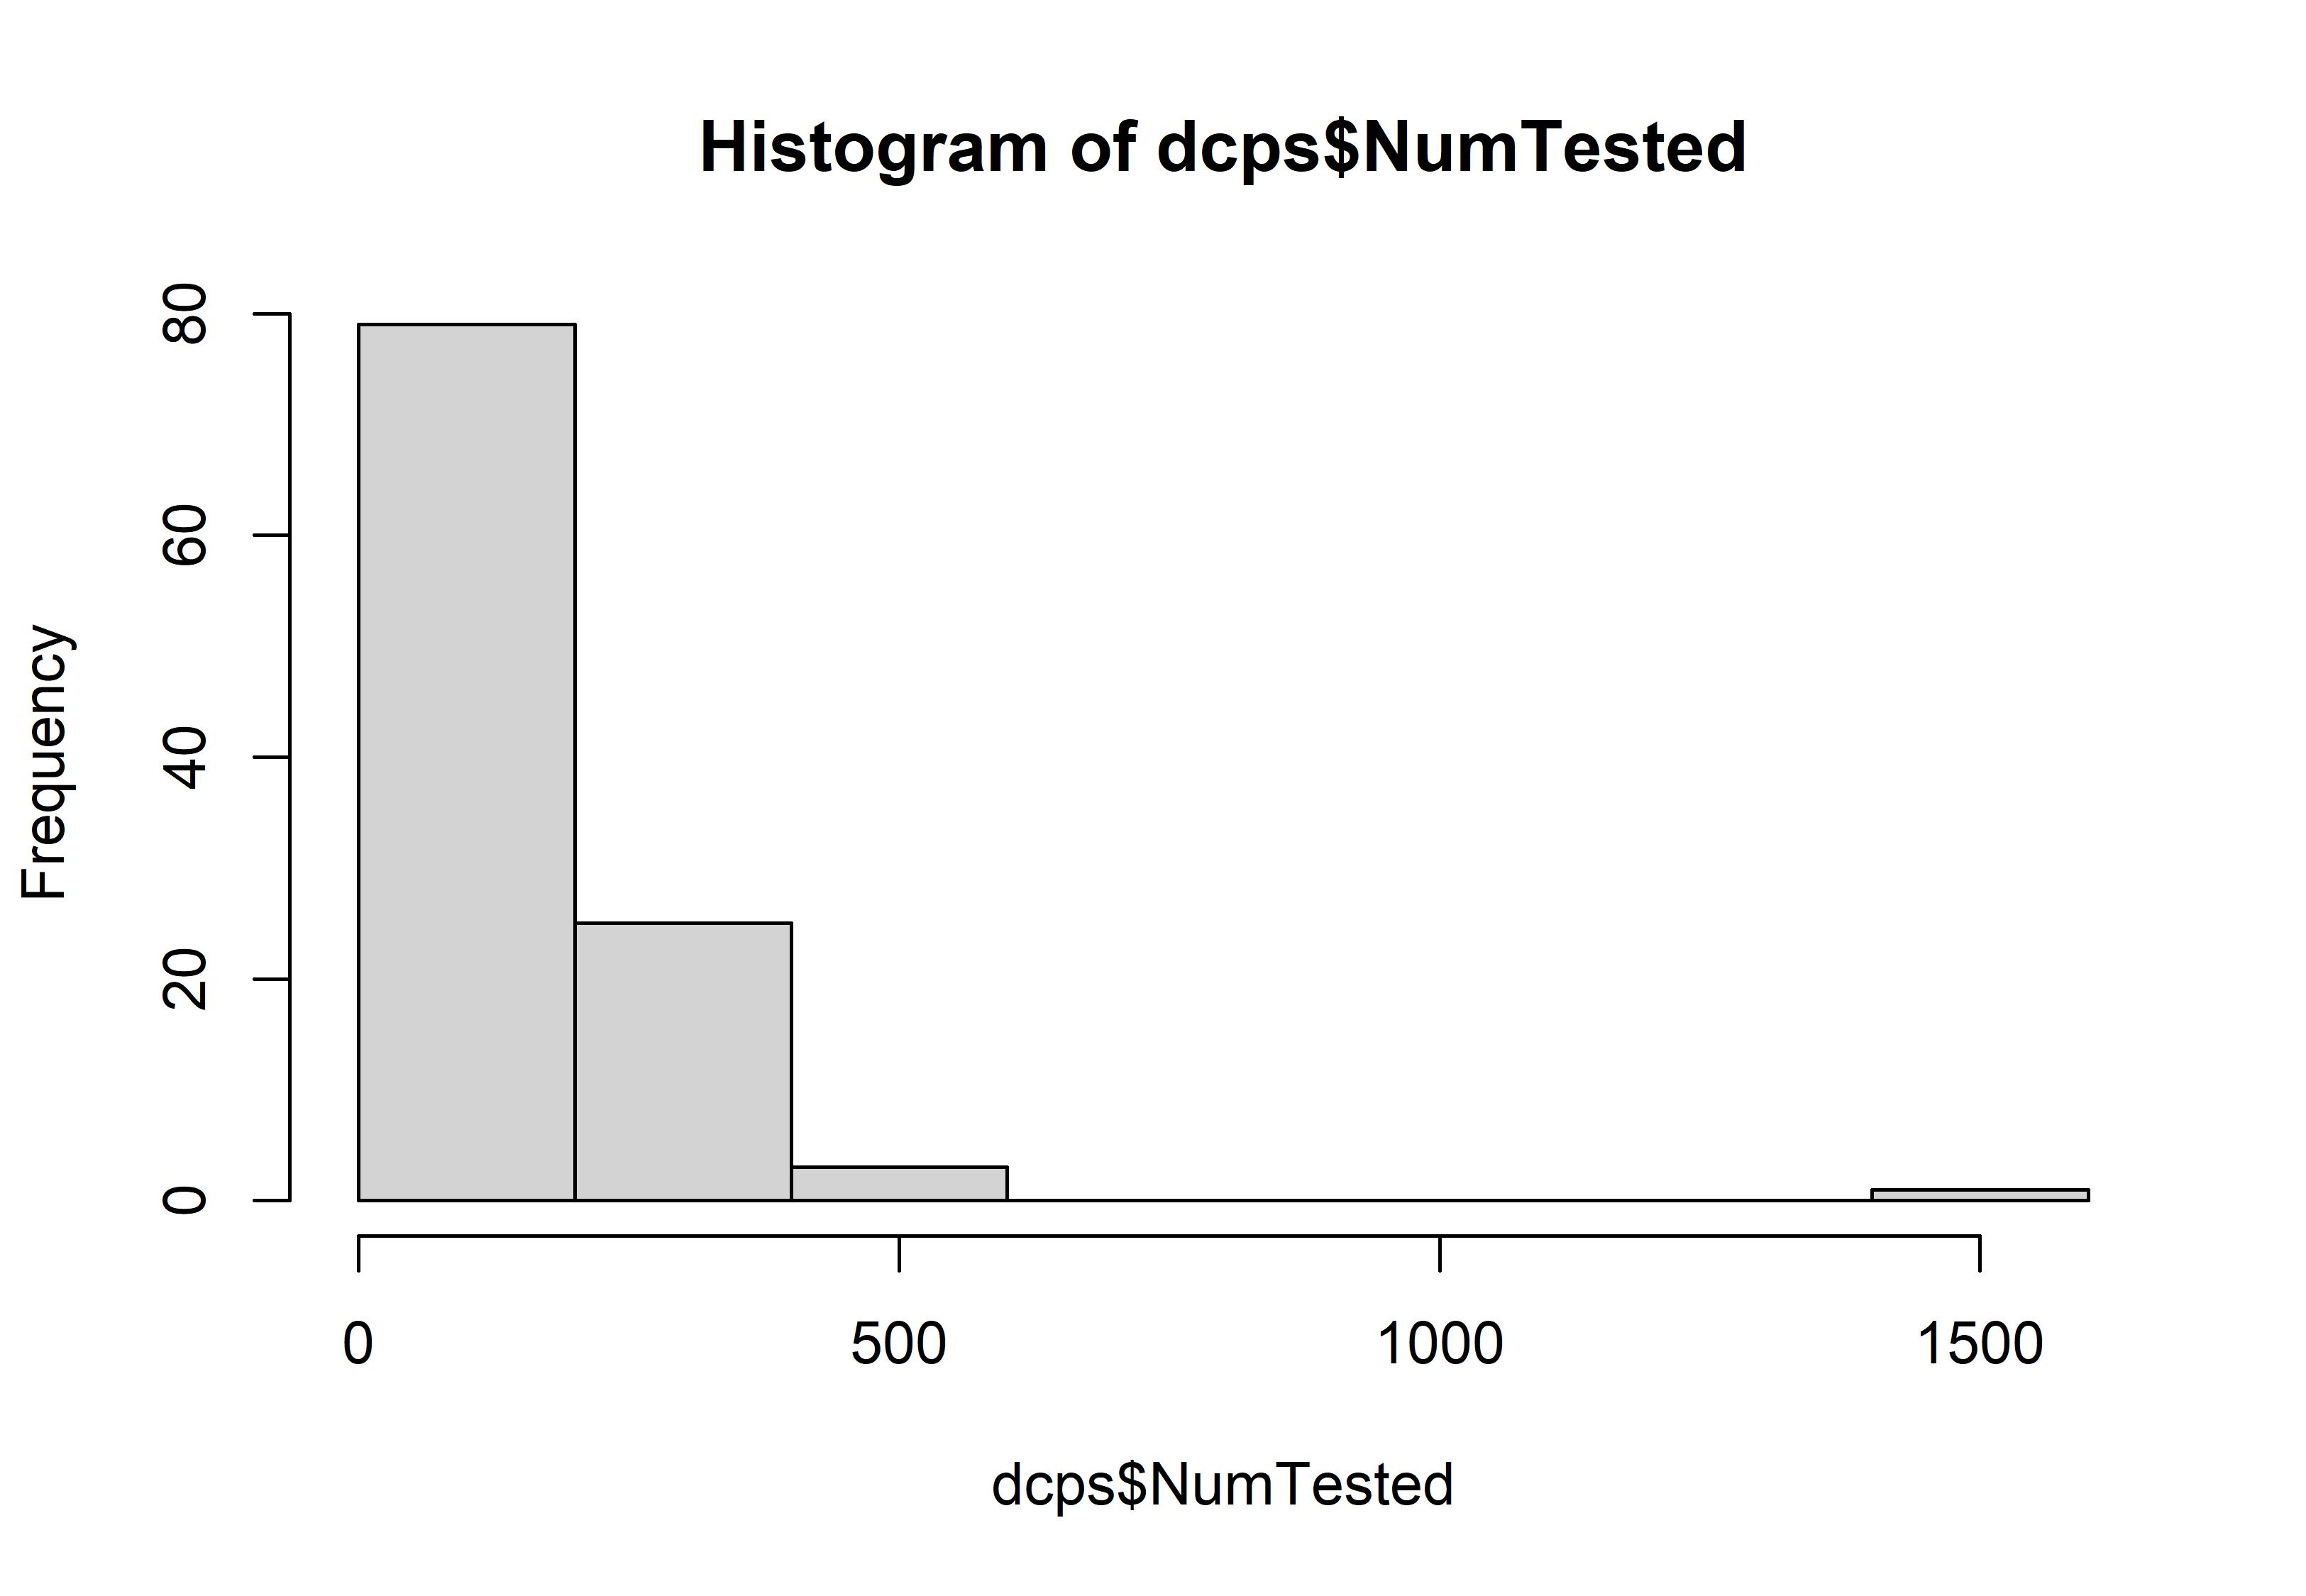
\includegraphics[width=0.4\linewidth]{SurvivR_files/figure-latex/basesum1-1} \end{center}

\begin{Shaded}
\begin{Highlighting}[]
  
\CommentTok{\# Boxplot (numeric X)  }
  \FunctionTok{boxplot}\NormalTok{(dcps}\SpecialCharTok{$}\NormalTok{ProfMath, }\AttributeTok{horizontal =} \ConstantTok{TRUE}\NormalTok{)}
\end{Highlighting}
\end{Shaded}

\begin{center}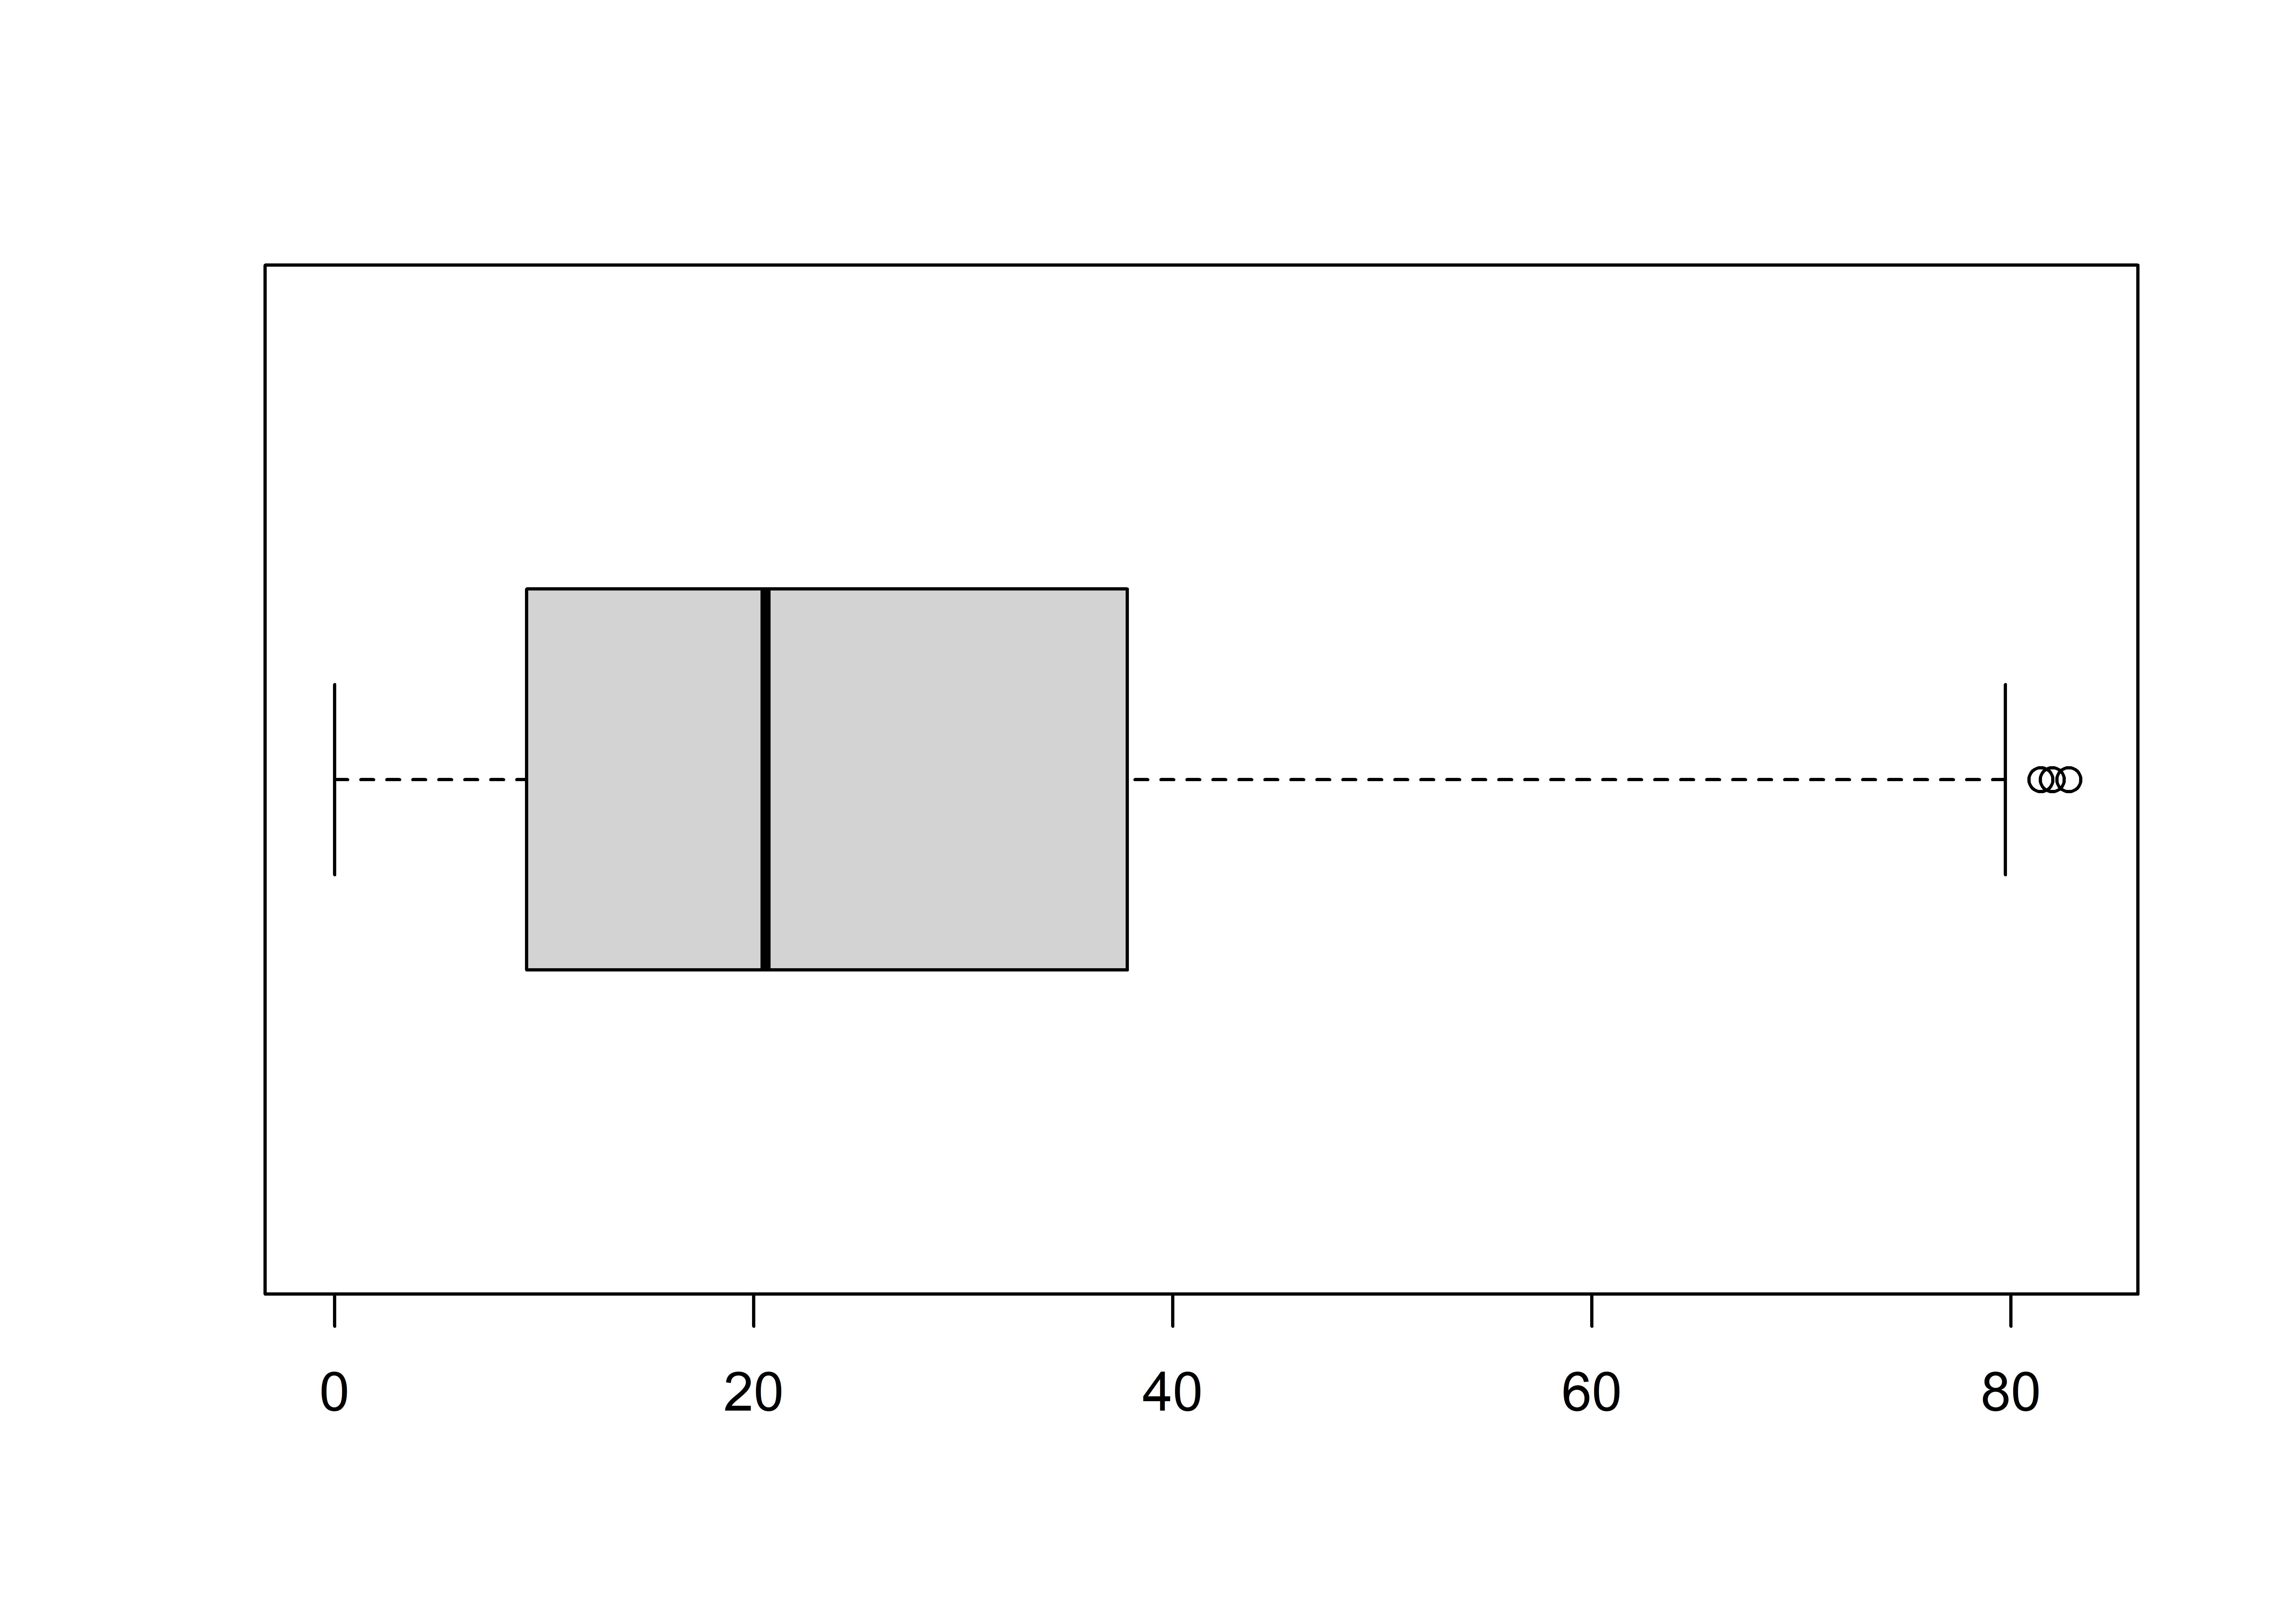
\includegraphics[width=0.4\linewidth]{SurvivR_files/figure-latex/basesum1-2} \end{center}

\begin{Shaded}
\begin{Highlighting}[]

\CommentTok{\# Bar plot (nominal X)}
  \CommentTok{\# 1. relative frequency table}
\NormalTok{    tab }\OtherTok{=} 
\NormalTok{      dcps }\SpecialCharTok{\%\textgreater{}\%}
      \FunctionTok{count}\NormalTok{(SchType) }\SpecialCharTok{\%\textgreater{}\%}
      \FunctionTok{mutate}\NormalTok{(}\AttributeTok{Percent =} \DecValTok{100} \SpecialCharTok{*}\NormalTok{ n}\SpecialCharTok{/}\FunctionTok{sum}\NormalTok{(n))}
    
  \CommentTok{\# 2. barplot from table}
    \FunctionTok{barplot}\NormalTok{(Percent }\SpecialCharTok{\textasciitilde{}}\NormalTok{ SchType, }\AttributeTok{data =}\NormalTok{ tab)}
\end{Highlighting}
\end{Shaded}

\begin{center}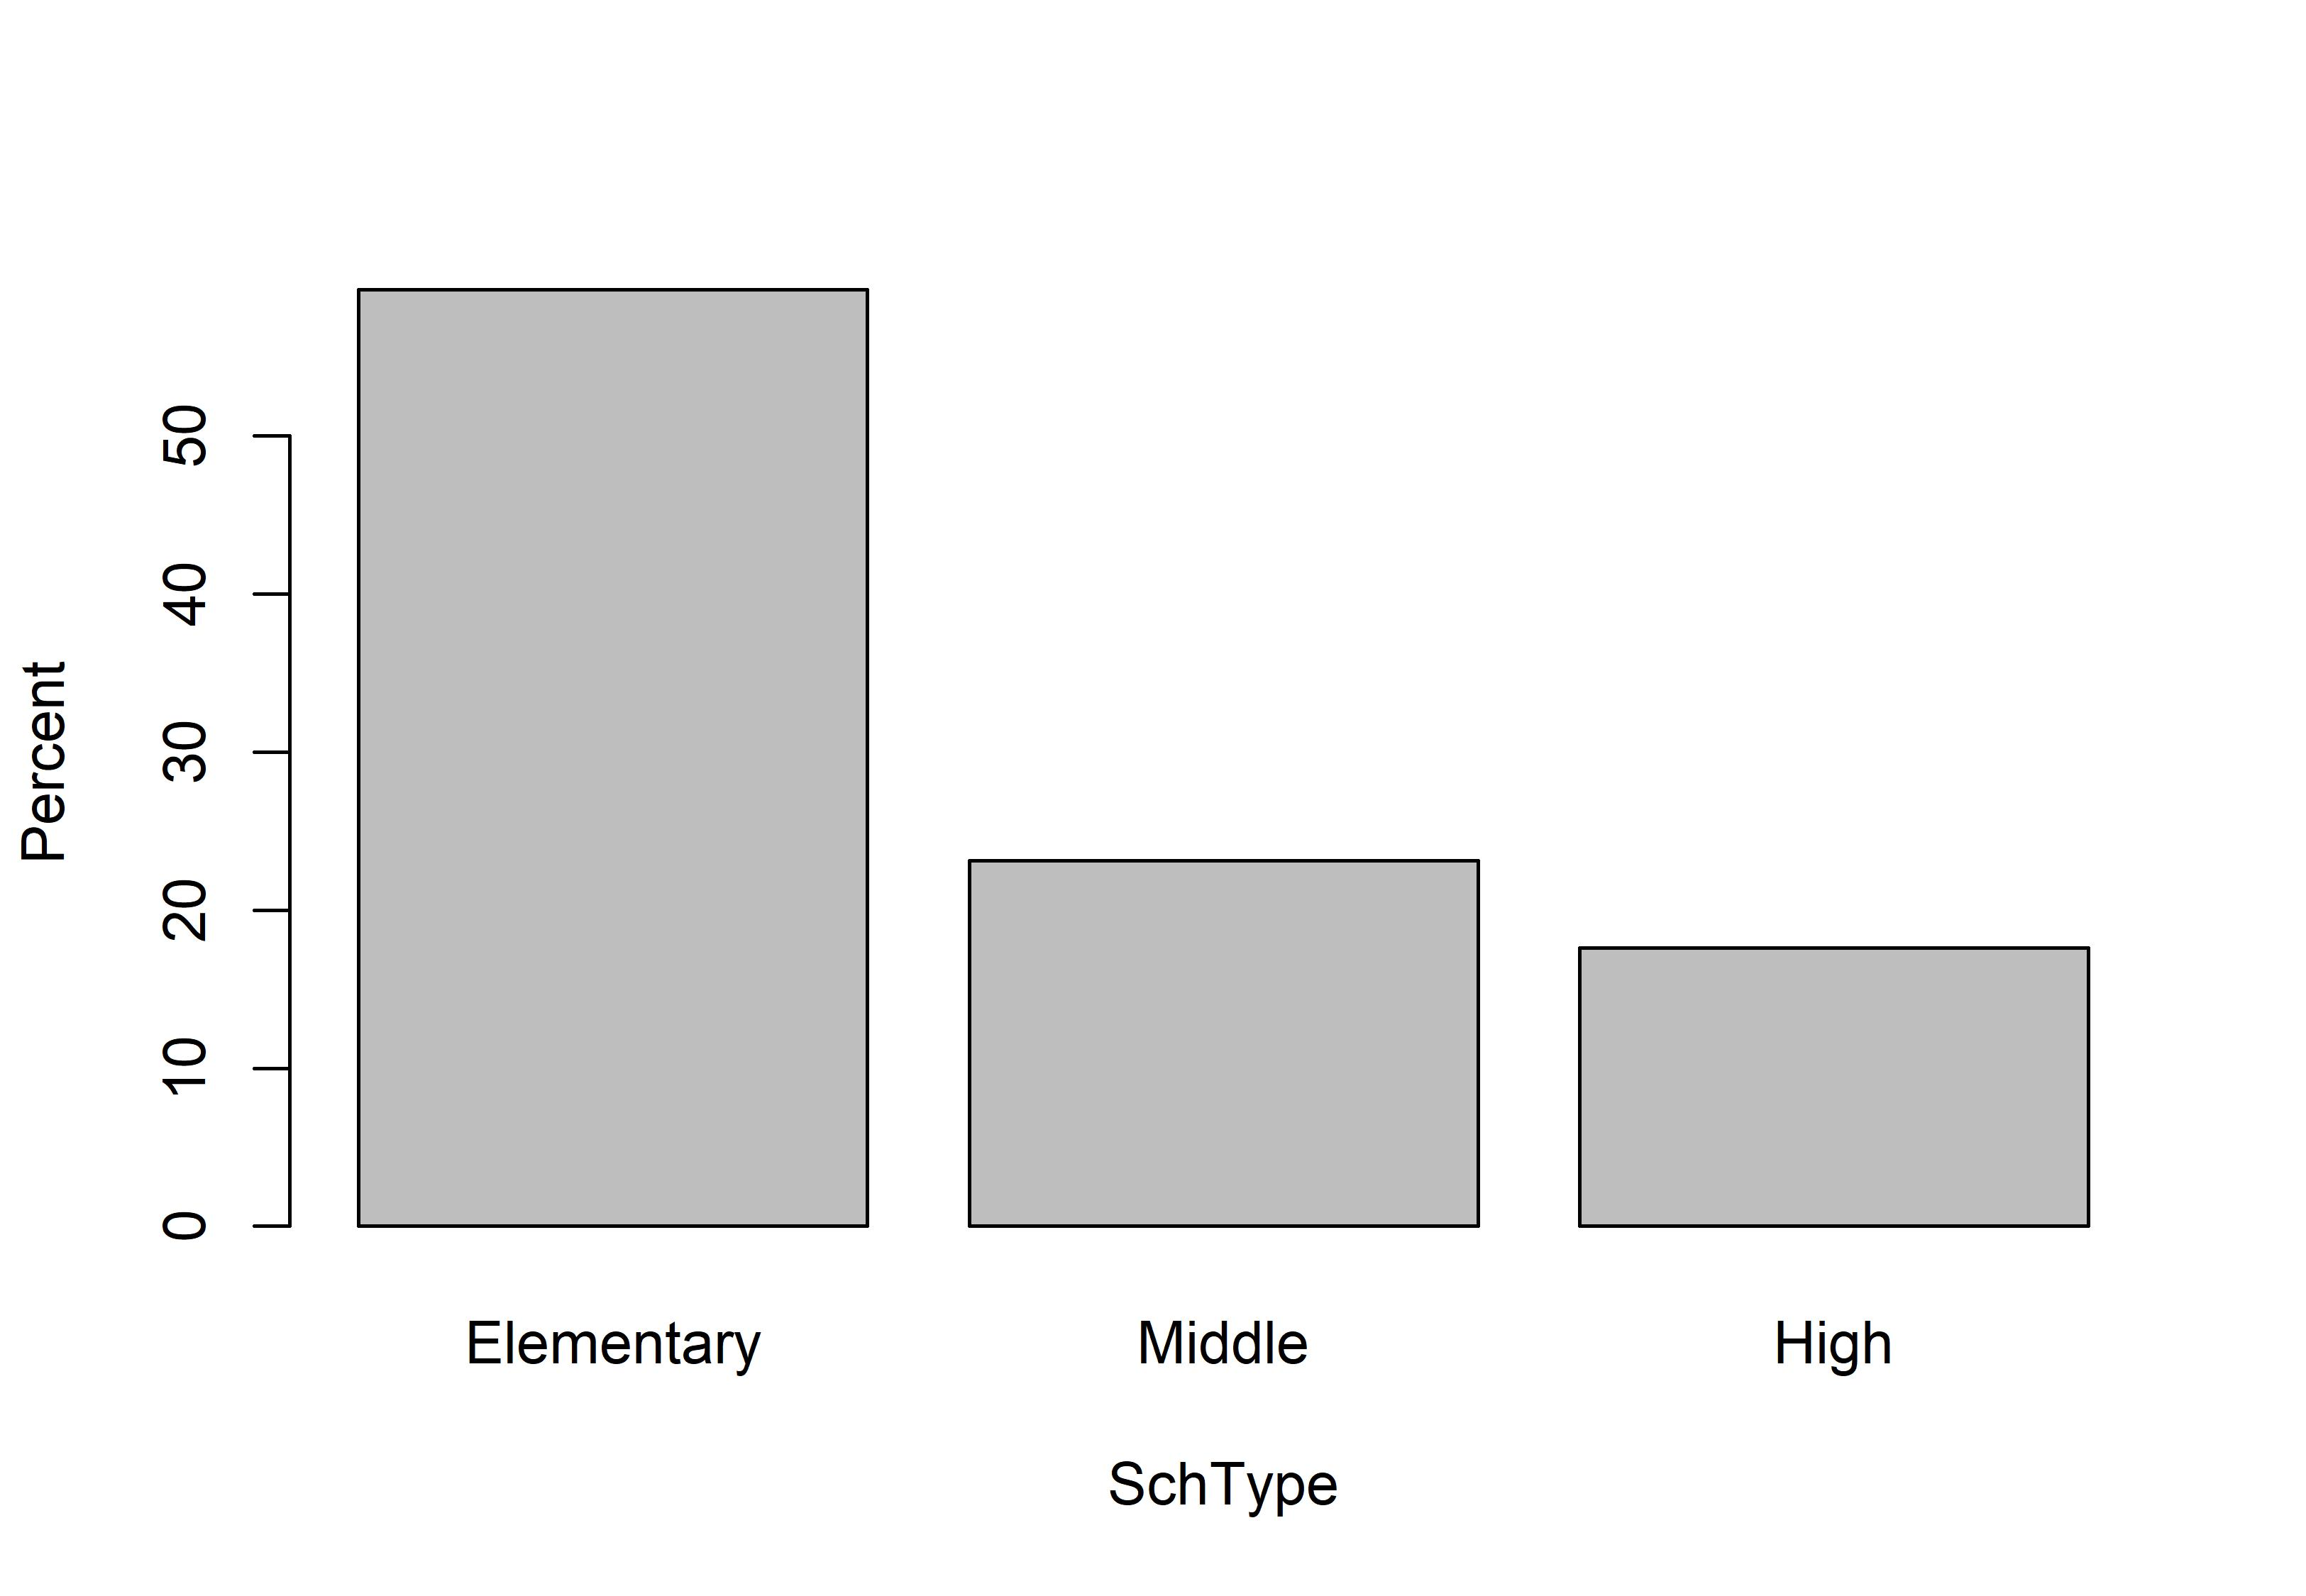
\includegraphics[width=0.4\linewidth]{SurvivR_files/figure-latex/basesum1-3} \end{center}

\hypertarget{visualizing-relationships}{%
\subsection{Visualizing relationships}\label{visualizing-relationships}}

For visualizing relationships between variables:

\begin{Shaded}
\begin{Highlighting}[]
\CommentTok{\# Group comparison (numeric X, nominal Y)}
  \FunctionTok{boxplot}\NormalTok{(NumTested }\SpecialCharTok{\textasciitilde{}}\NormalTok{ SchType, }\AttributeTok{data =}\NormalTok{ dcps)}
\end{Highlighting}
\end{Shaded}

\begin{center}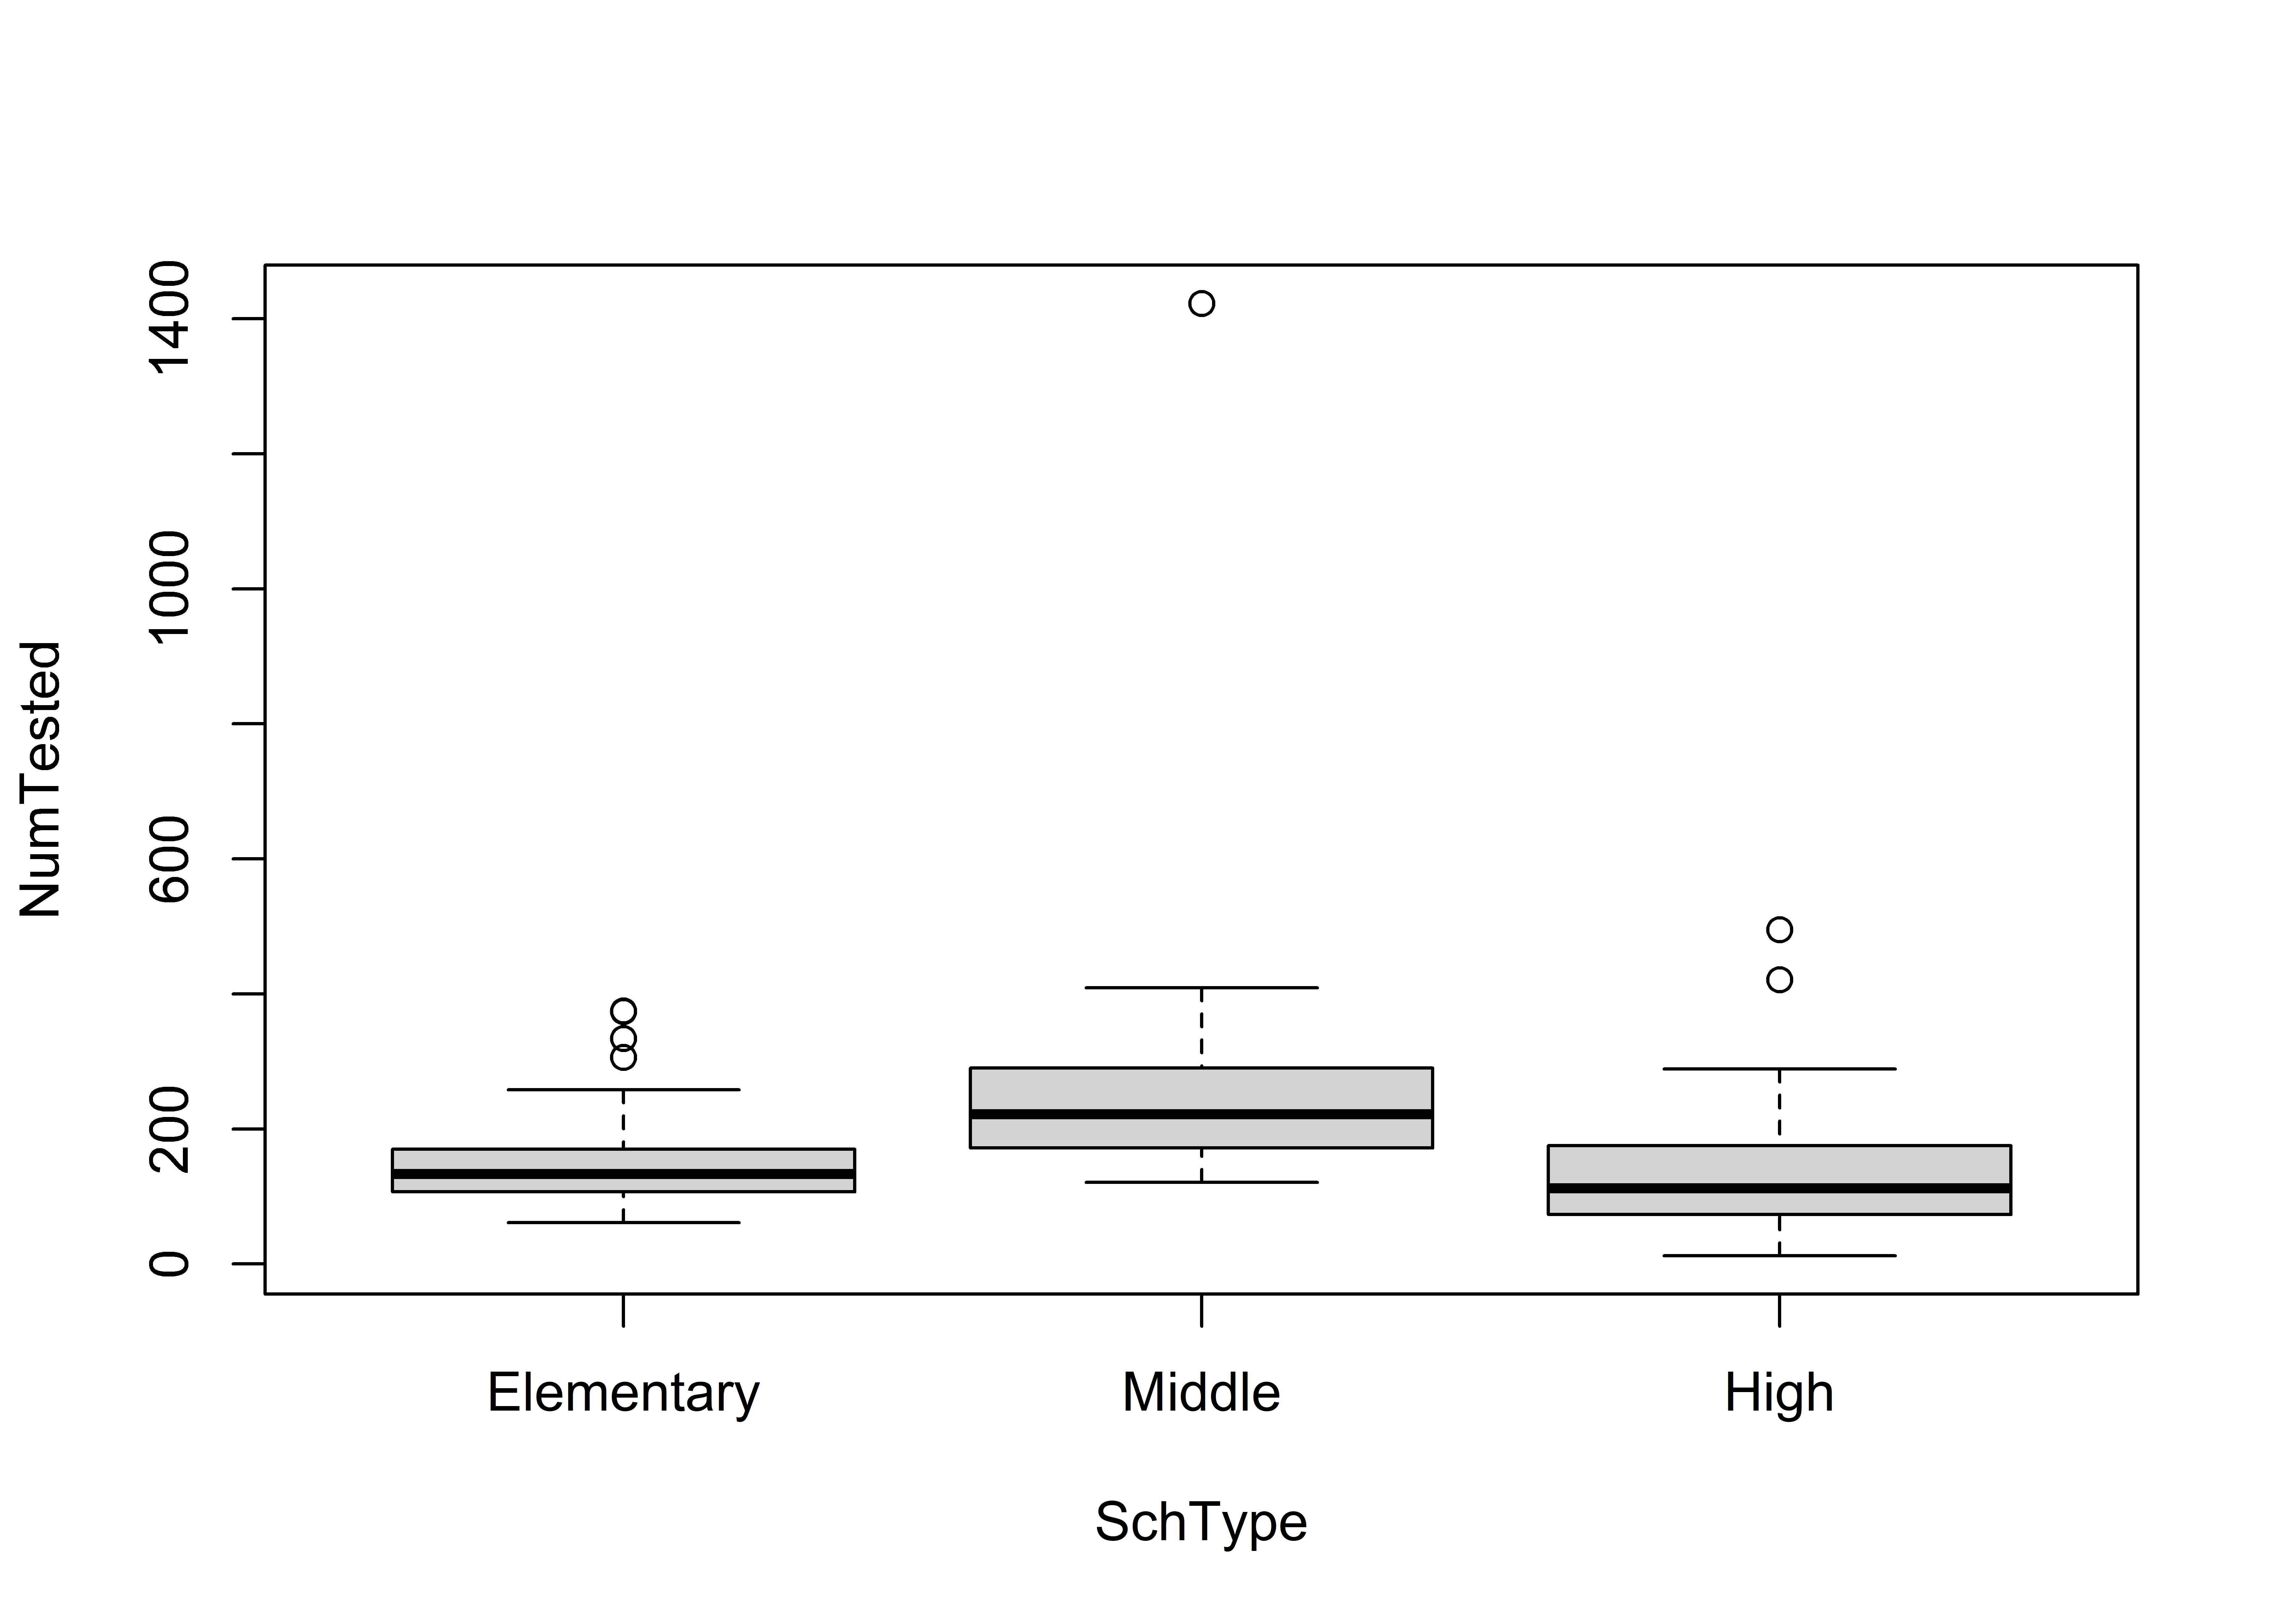
\includegraphics[width=0.4\linewidth]{SurvivR_files/figure-latex/basesum2-1} \end{center}

\begin{Shaded}
\begin{Highlighting}[]
  
\CommentTok{\# Scatter plot (numeric X, numeric Y)}
  \FunctionTok{plot}\NormalTok{(ProfLang }\SpecialCharTok{\textasciitilde{}}\NormalTok{ SchType, }\AttributeTok{data =}\NormalTok{ dcps)}
\end{Highlighting}
\end{Shaded}

\begin{center}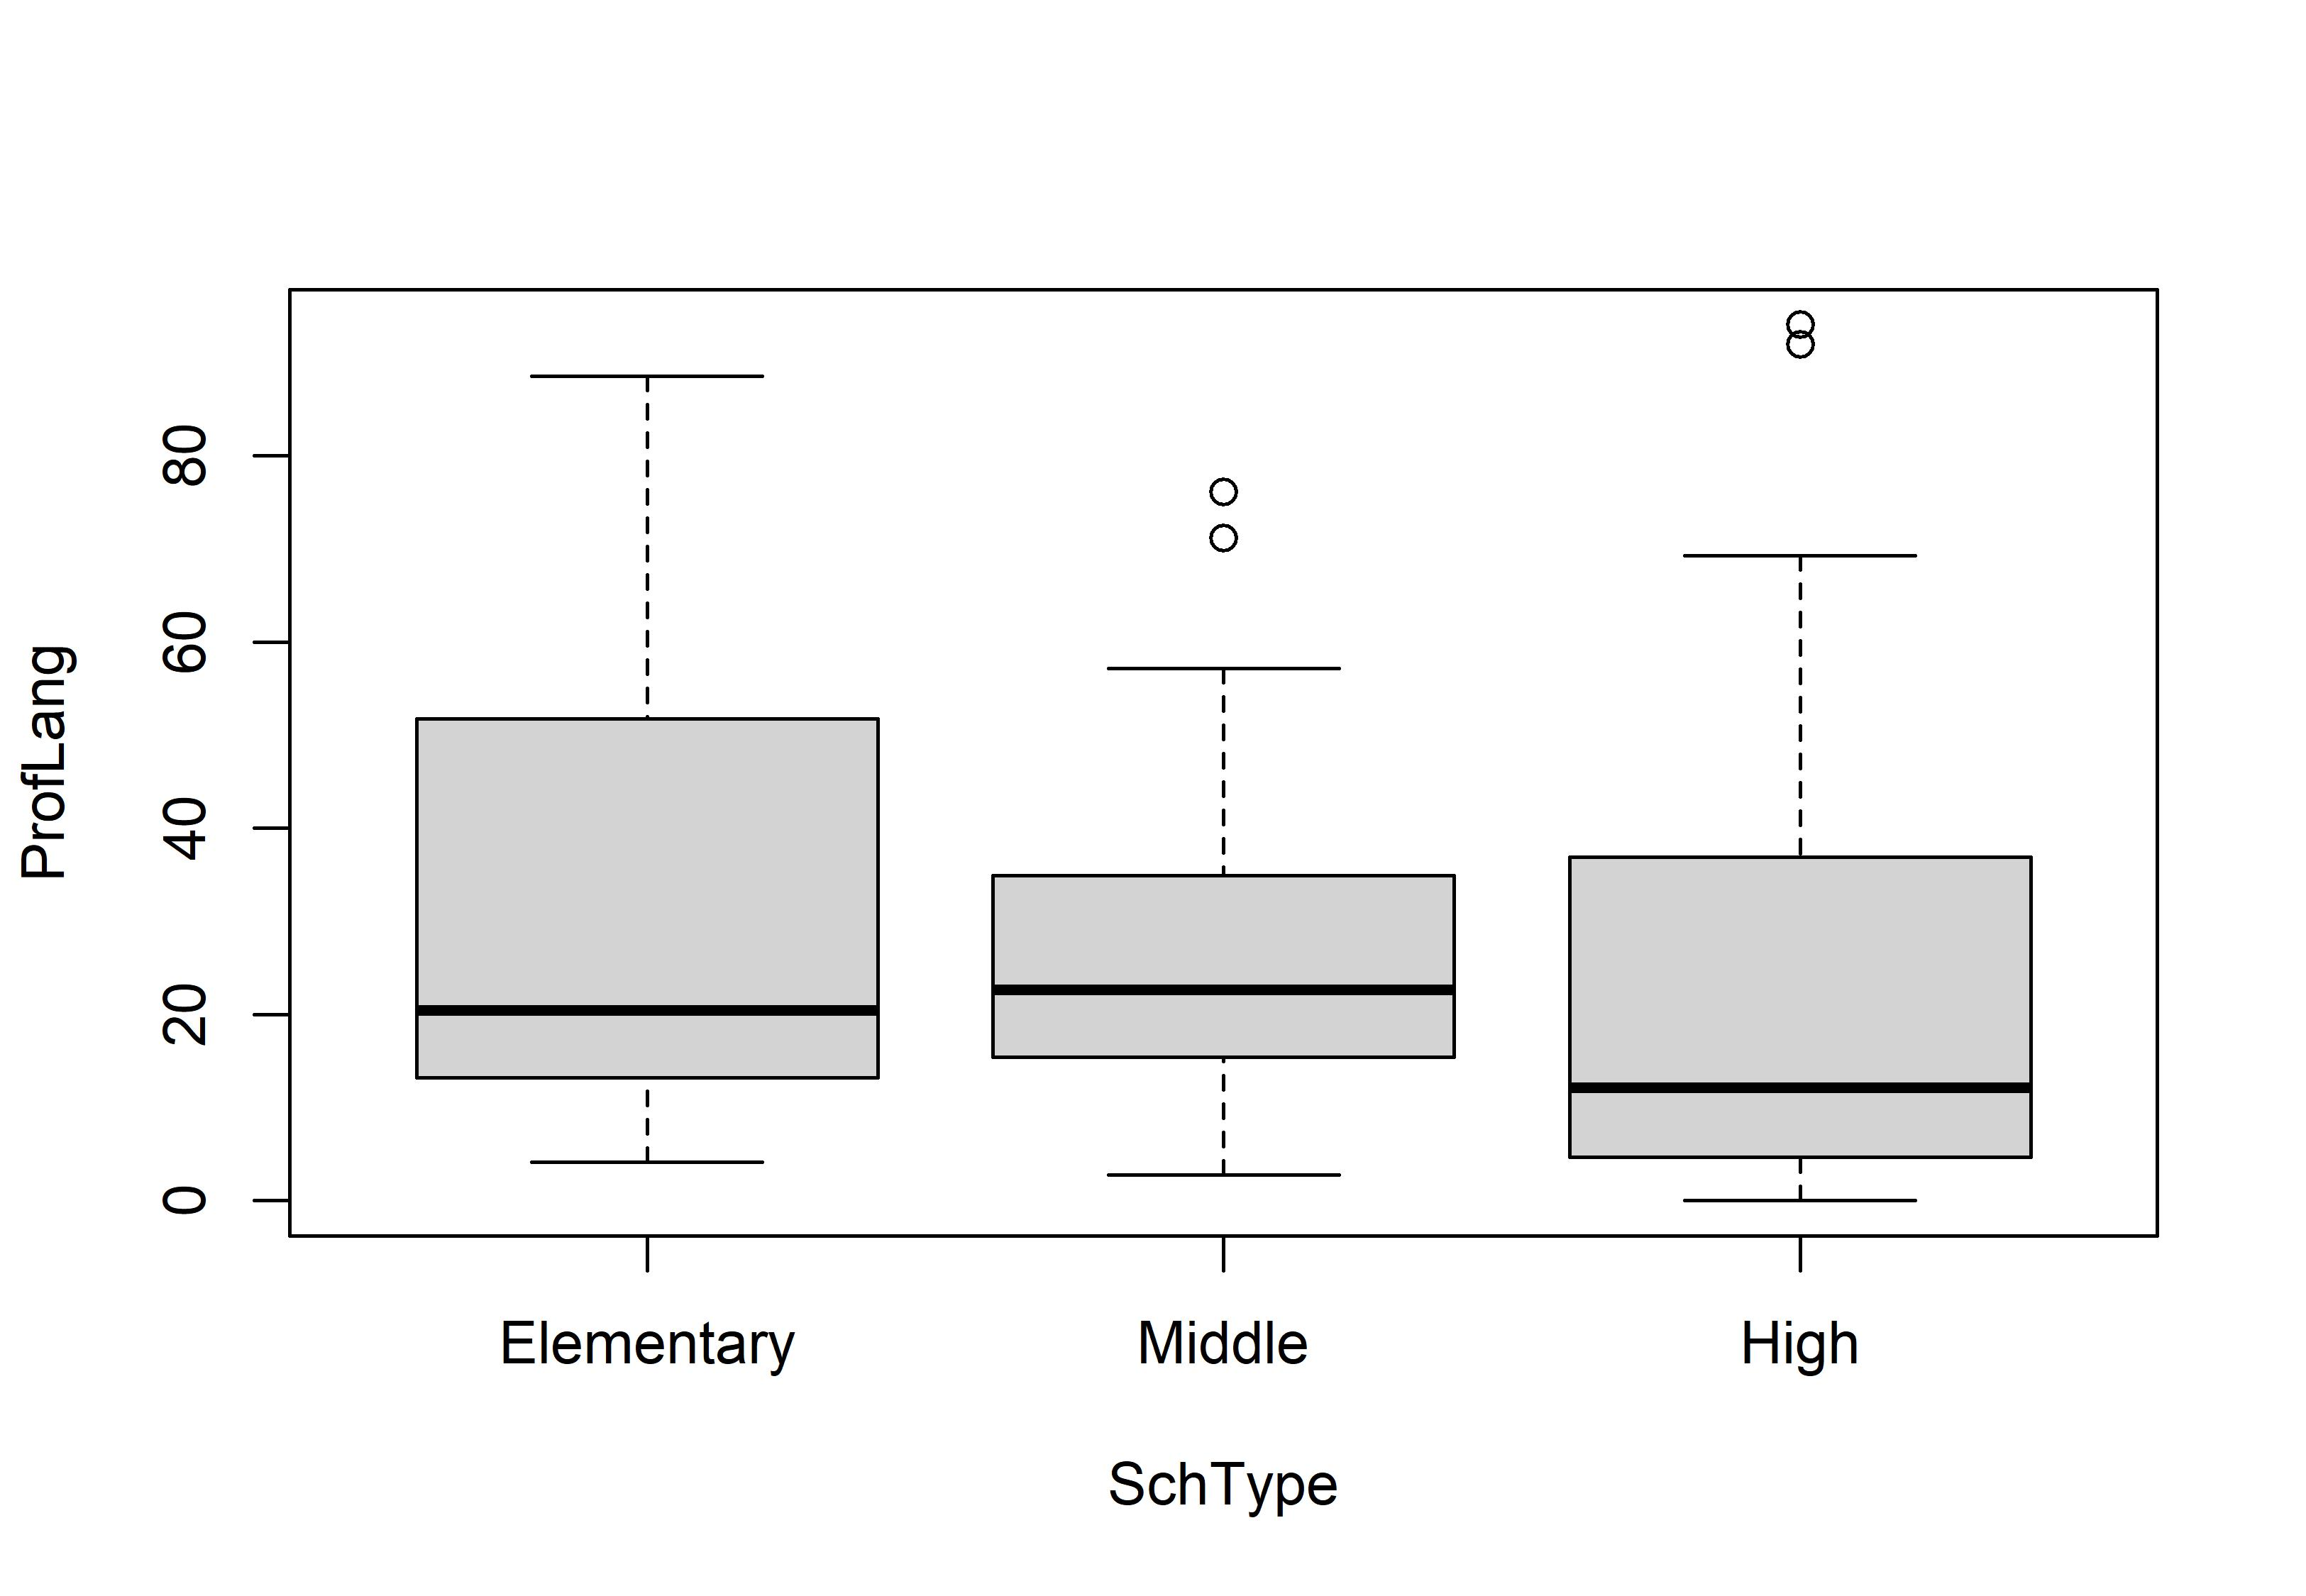
\includegraphics[width=0.4\linewidth]{SurvivR_files/figure-latex/basesum2-2} \end{center}

\begin{Shaded}
\begin{Highlighting}[]

\CommentTok{\# Scatter w/OLS fit (numeric X, numeric Y)}
  \CommentTok{\# 1. store OLS estimates}
\NormalTok{    est }\OtherTok{=} \FunctionTok{lm}\NormalTok{(ProfLang }\SpecialCharTok{\textasciitilde{}}\NormalTok{ ProfMath, }\AttributeTok{data =}\NormalTok{ dcps)}
  \CommentTok{\# 2. plot  }
    \FunctionTok{plot}\NormalTok{(ProfLang }\SpecialCharTok{\textasciitilde{}}\NormalTok{ ProfMath, }\AttributeTok{data =}\NormalTok{ dcps) }\CommentTok{\# scatter}
    \FunctionTok{abline}\NormalTok{(est) }\CommentTok{\# add linear fit}
\end{Highlighting}
\end{Shaded}

\begin{center}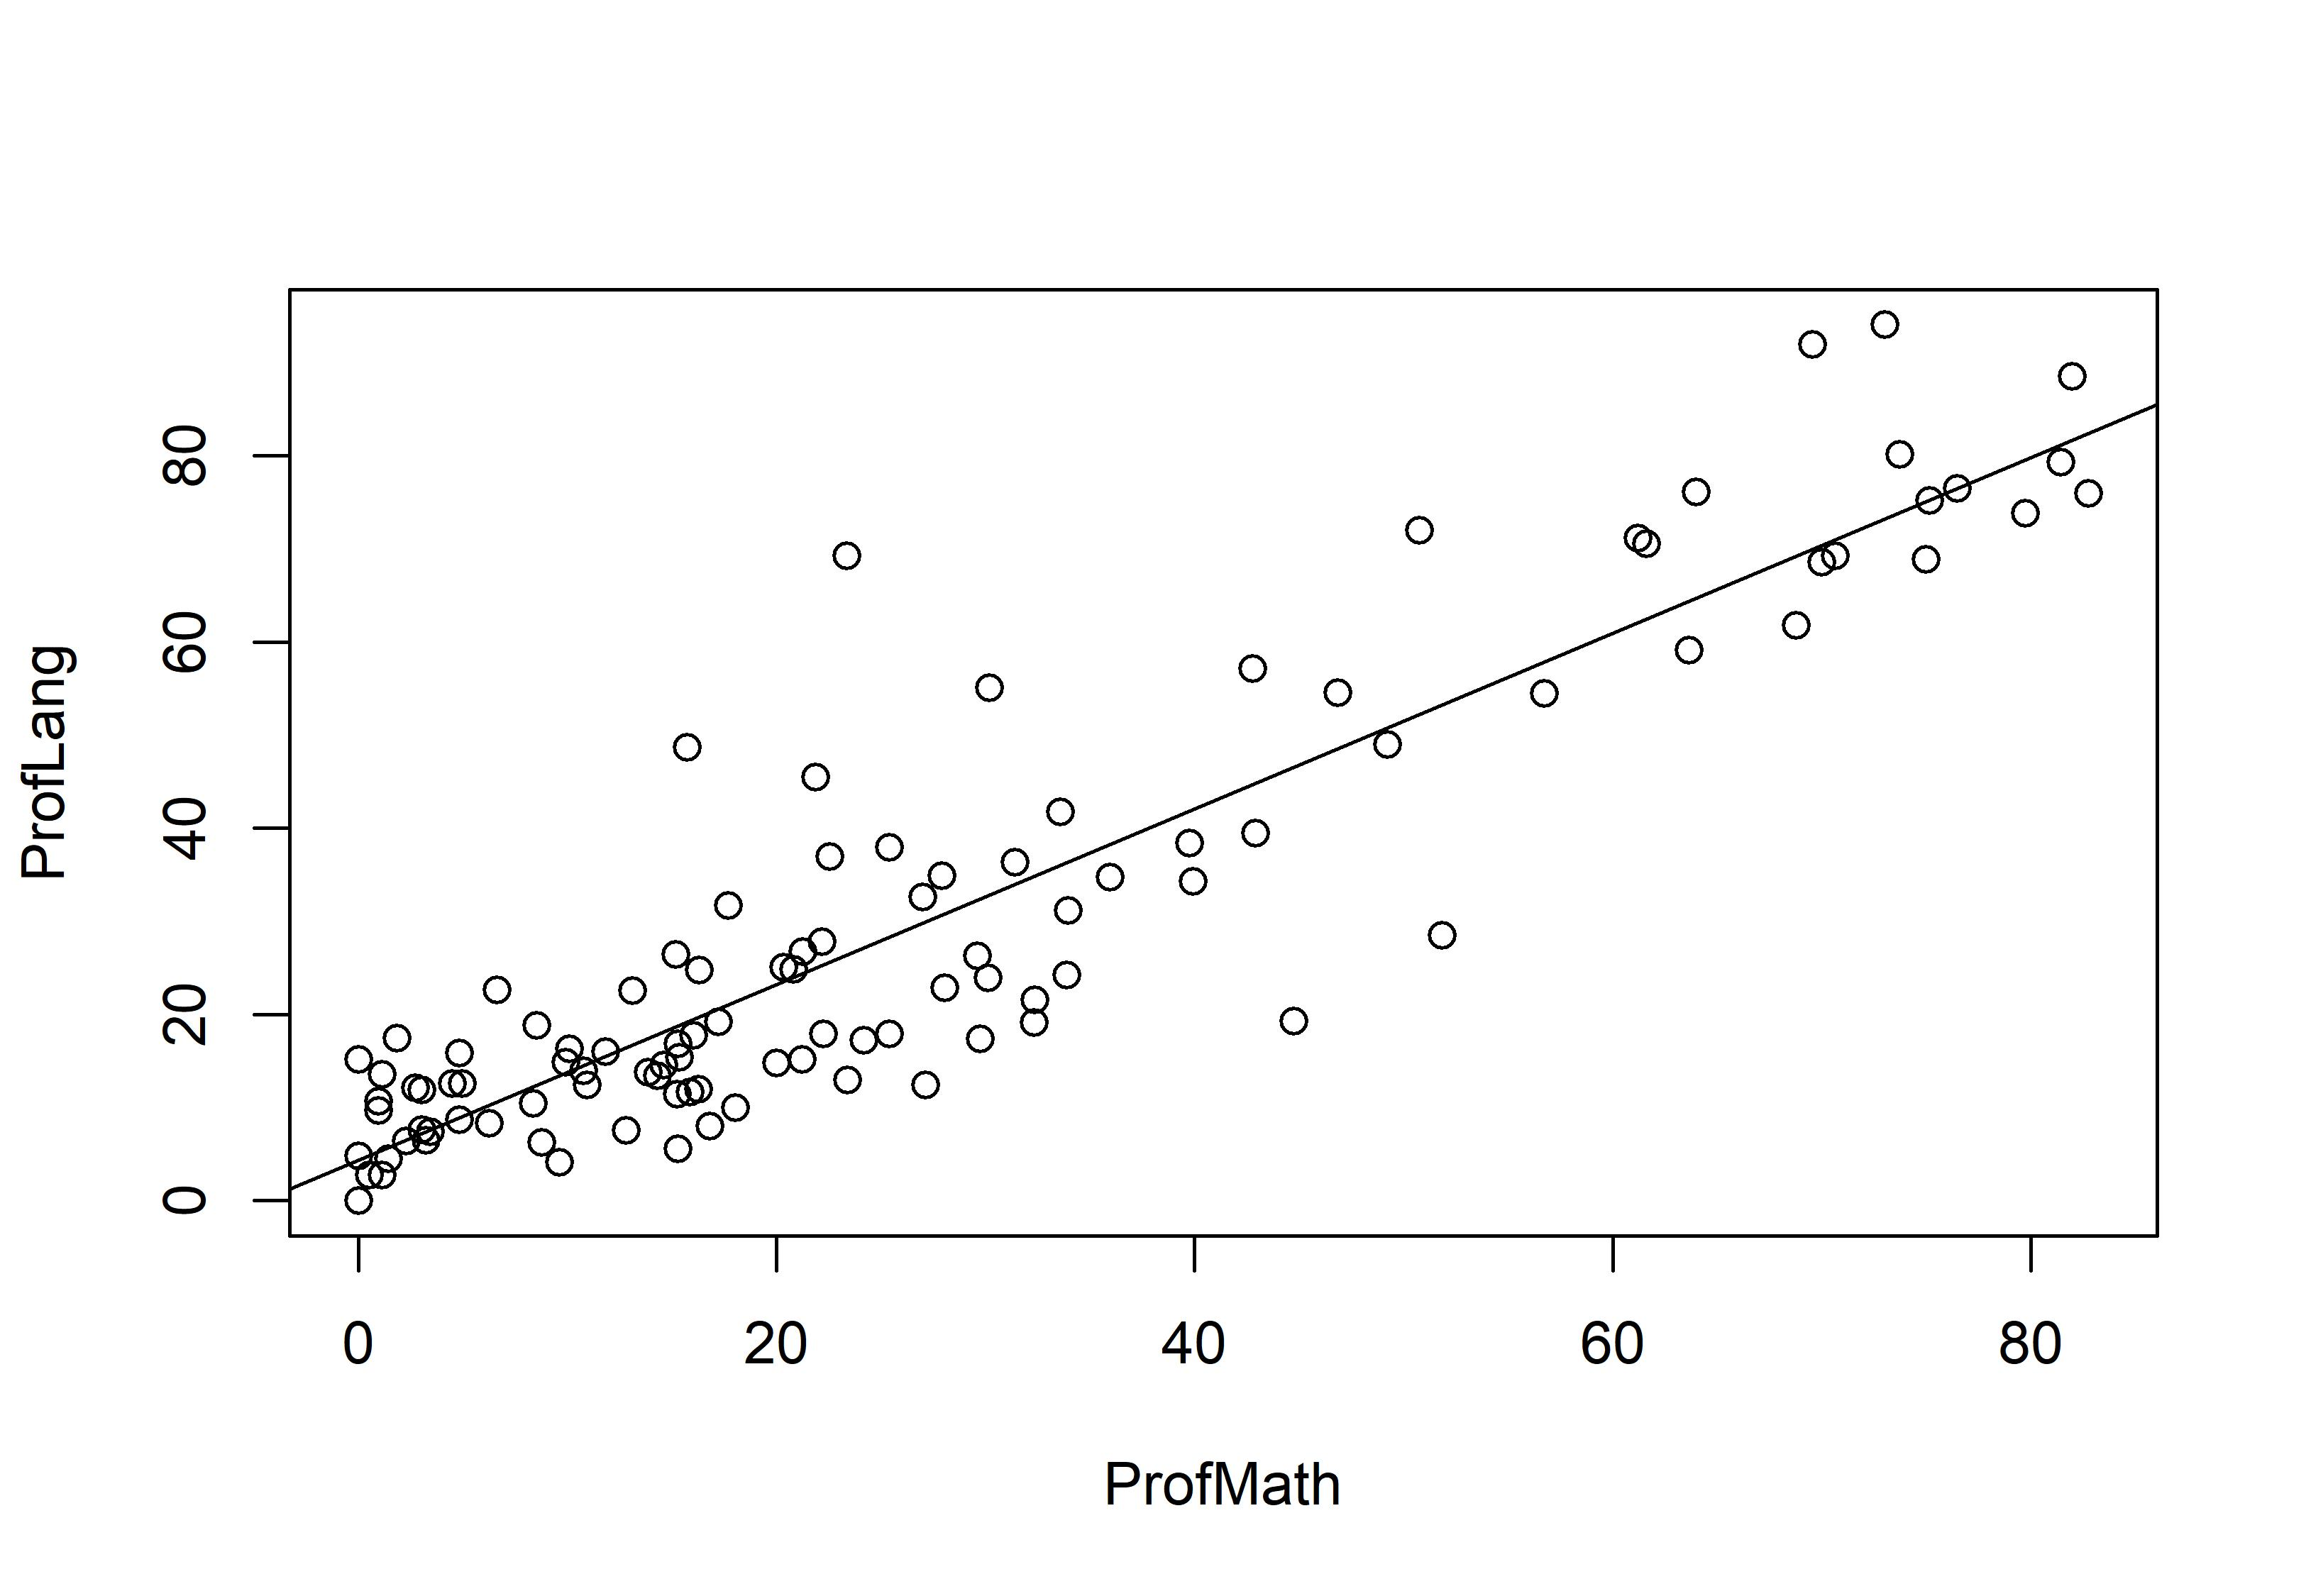
\includegraphics[width=0.4\linewidth]{SurvivR_files/figure-latex/basesum2-3} \end{center}

\hypertarget{professional-formatting}{%
\section{Professional formatting}\label{professional-formatting}}

Formatting is what differentiates an exploratory graph from one you would present to others. The options for formatting an R graphic are almost limitless. However, of special importance are the descriptive text (e.g.~titles), axis scales, and the graphical parameters (e.g.~color and shape of the points).

I suggest the \href{https://www.statmethods.net/advgraphs/index.html}{Quick-R Advanced Graphs page} for more details and for more advanced examples.

\hypertarget{titles-and-labels}{%
\subsection{Titles and labels}\label{titles-and-labels}}

Within the different plotting functions, you can specify the main title (\texttt{main\ =}), axis labels (e.g.~\texttt{xlab\ =}), and more. Choose simple, descriptive labels and titles.

\begin{Shaded}
\begin{Highlighting}[]
  \FunctionTok{hist}\NormalTok{(dcps}\SpecialCharTok{$}\NormalTok{ProfLang,}
       \AttributeTok{main =} \StringTok{"Language Proficiency, DCPS 2018"}\NormalTok{,}
       \AttributeTok{xlab =} \StringTok{\textquotesingle{}Grade{-}level proficient (\% tested)\textquotesingle{}}\NormalTok{, }\AttributeTok{ylab =} \StringTok{\textquotesingle{}Frequency\textquotesingle{}}\NormalTok{)}
\end{Highlighting}
\end{Shaded}

\begin{center}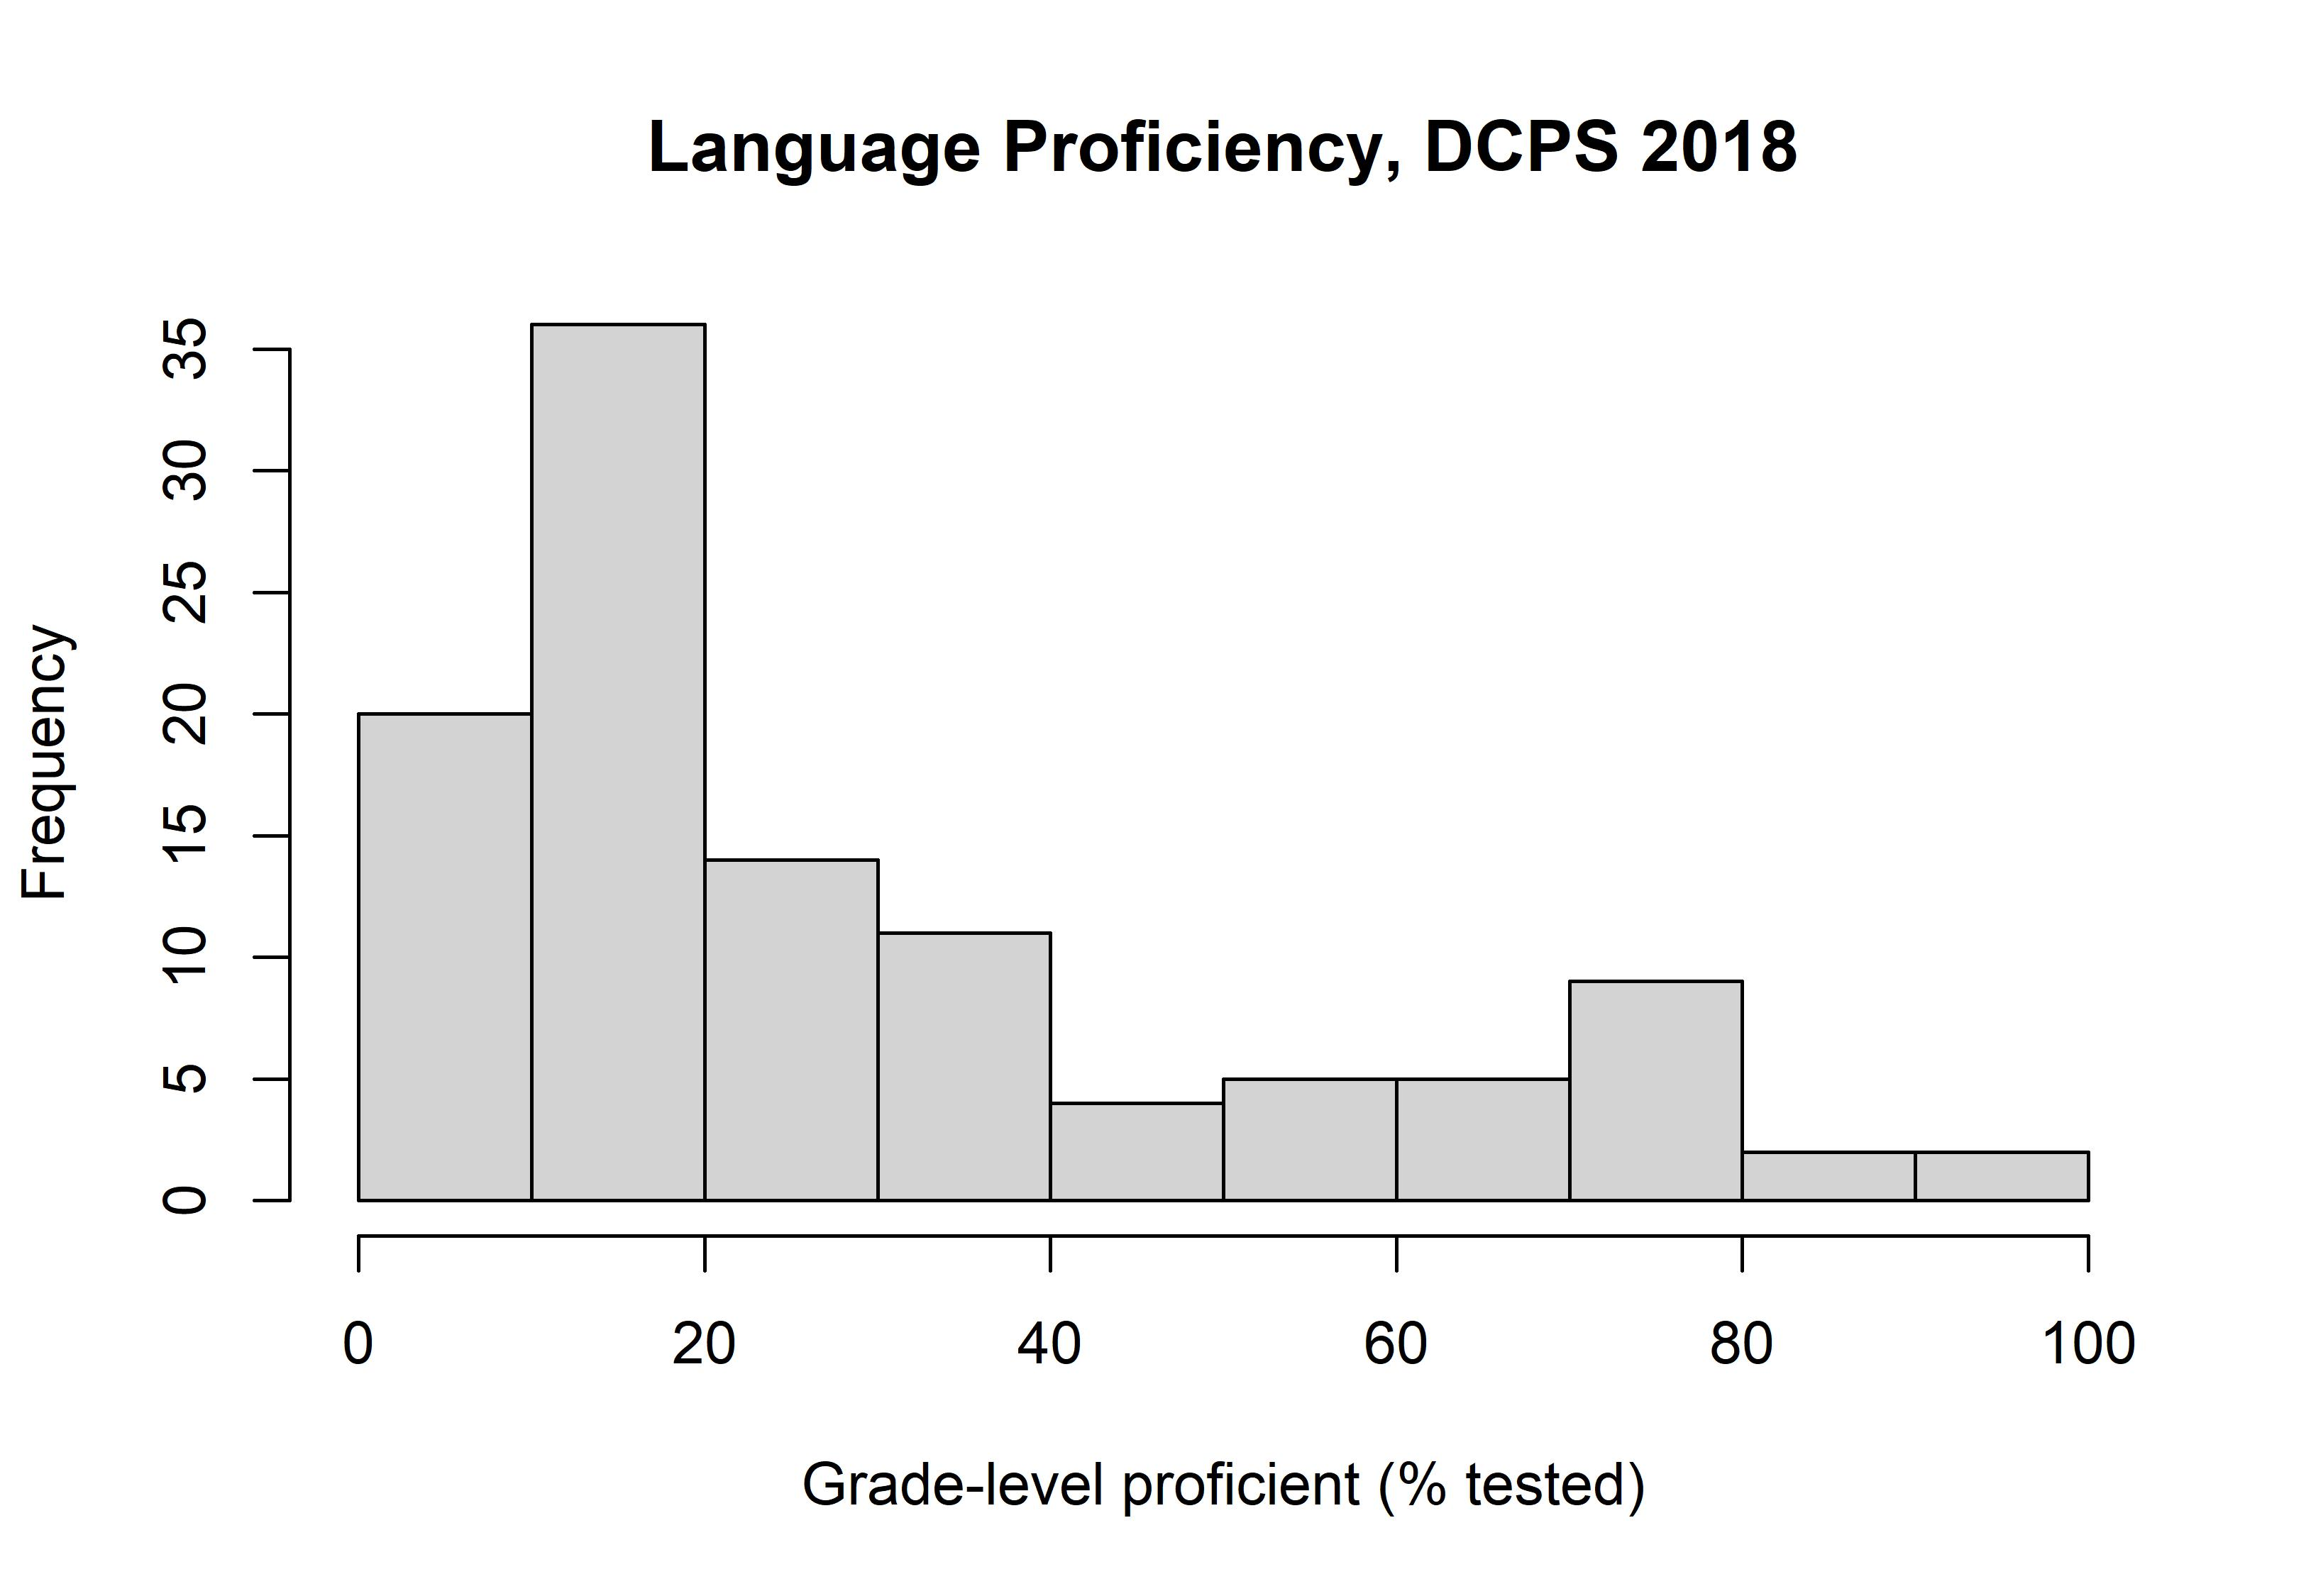
\includegraphics[width=0.4\linewidth]{SurvivR_files/figure-latex/titles-1} \end{center}

\hypertarget{axis-options}{%
\subsection{Axis options}\label{axis-options}}

Sometimes the axis scales that R chooses don't make sense or fail to communicate effectively. In these cases, we want to format the endpoints, or limits, of each axis scale. You do this using \texttt{xlim} and \texttt{ylim}, which allow you to specify a custom minimum and maximum value on each axis (e.g.~\texttt{xlim\ =\ c(min,max)}). Note that you must provide both using the appropriate syntax.

\begin{Shaded}
\begin{Highlighting}[]
  \FunctionTok{plot}\NormalTok{(ProfLang }\SpecialCharTok{\textasciitilde{}}\NormalTok{ NumTested, }\AttributeTok{data =}\NormalTok{ dcps,}
       \AttributeTok{xlim =} \FunctionTok{c}\NormalTok{(}\DecValTok{0}\NormalTok{,}\DecValTok{1500}\NormalTok{), }\AttributeTok{ylim =} \FunctionTok{c}\NormalTok{(}\DecValTok{0}\NormalTok{,}\DecValTok{100}\NormalTok{)) }\CommentTok{\# boundaries on X and Y}
\end{Highlighting}
\end{Shaded}

\begin{center}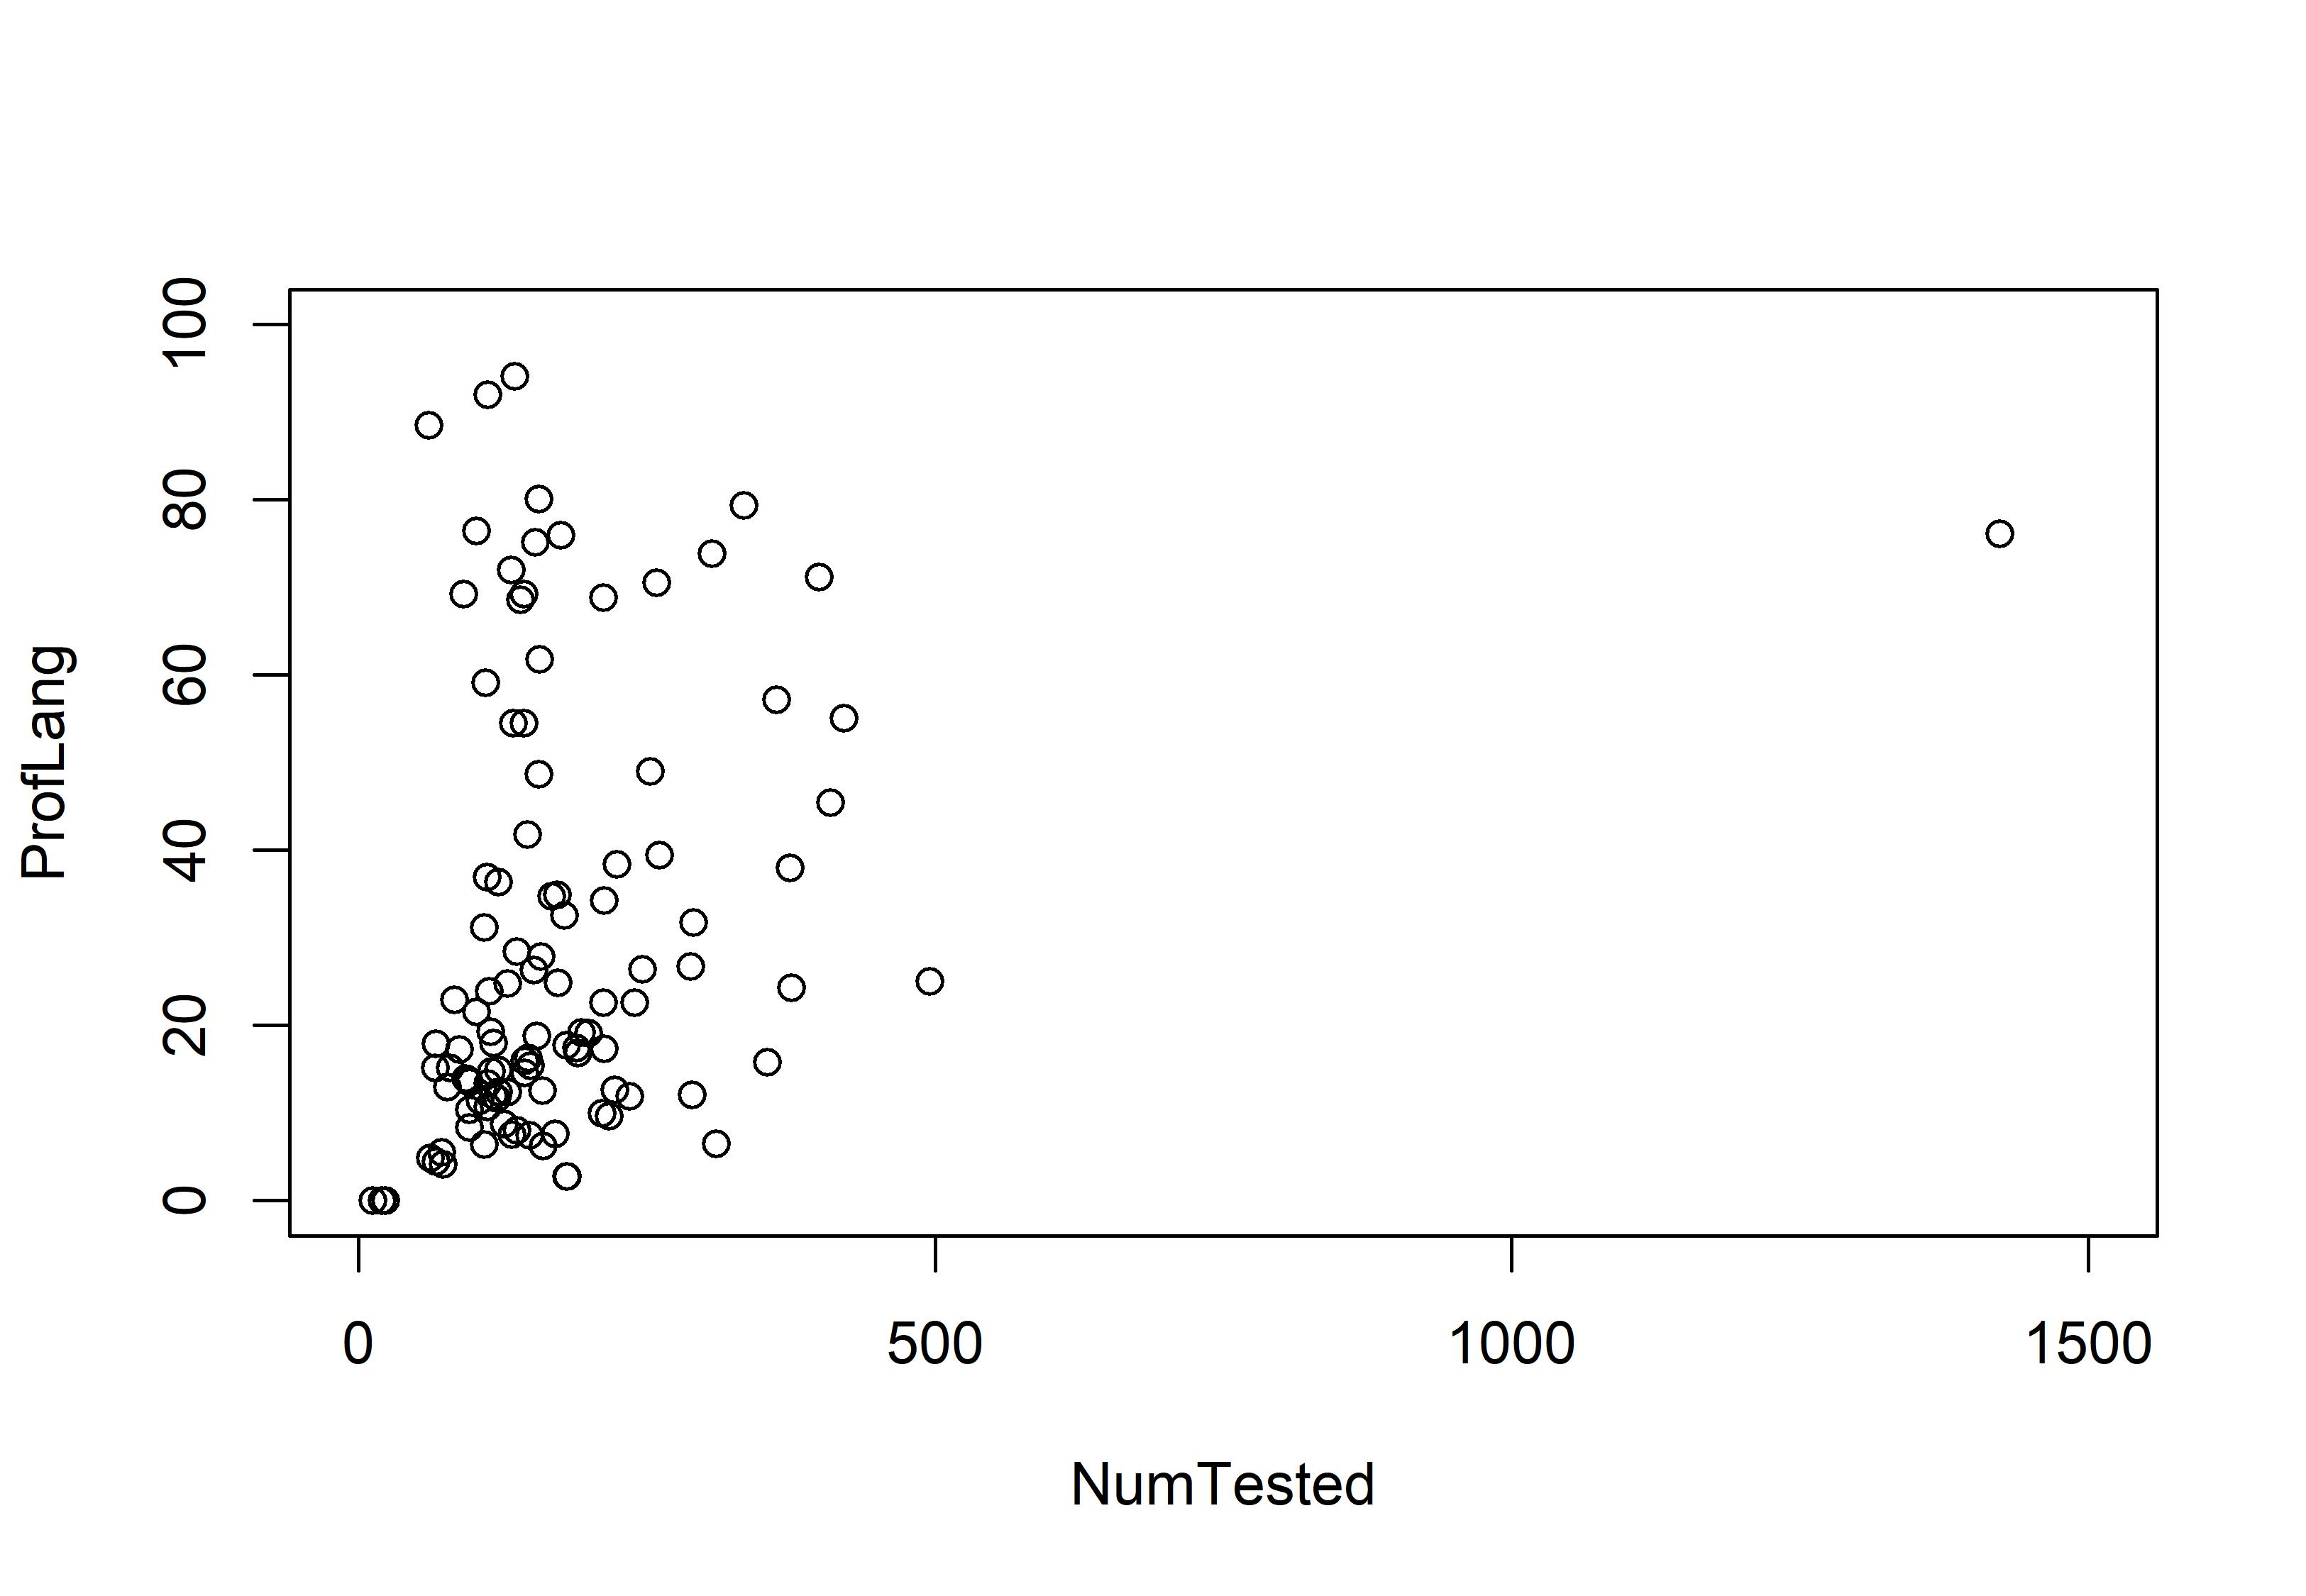
\includegraphics[width=0.4\linewidth]{SurvivR_files/figure-latex/axes-1} \end{center}

\hypertarget{graphical-parameters}{%
\subsection{Graphical parameters}\label{graphical-parameters}}

Basic R graphs are clean and sparse; these are important advantages. However, we may want to spice things up beyond the simple black and white. This is especially true in graphs with multiple components (e.g.~a scatter plot with linear fit) where color/shape contrast is important to differentiate the elements. See below examples of changing fill color (\texttt{col}), border color (\texttt{border}), point shape (\texttt{pch}), line type (\texttt{lty}), and line width (\texttt{lwd}).

\begin{Shaded}
\begin{Highlighting}[]
\CommentTok{\# Histogram (or boxplot)}
  \FunctionTok{hist}\NormalTok{(dcps}\SpecialCharTok{$}\NormalTok{ProfMath,}
       \AttributeTok{col =} \StringTok{\textquotesingle{}cornflowerblue\textquotesingle{}}\NormalTok{, }\CommentTok{\# fill color}
       \AttributeTok{border =} \StringTok{\textquotesingle{}deeppink4\textquotesingle{}}\NormalTok{) }\CommentTok{\# broder color}
\end{Highlighting}
\end{Shaded}

\begin{center}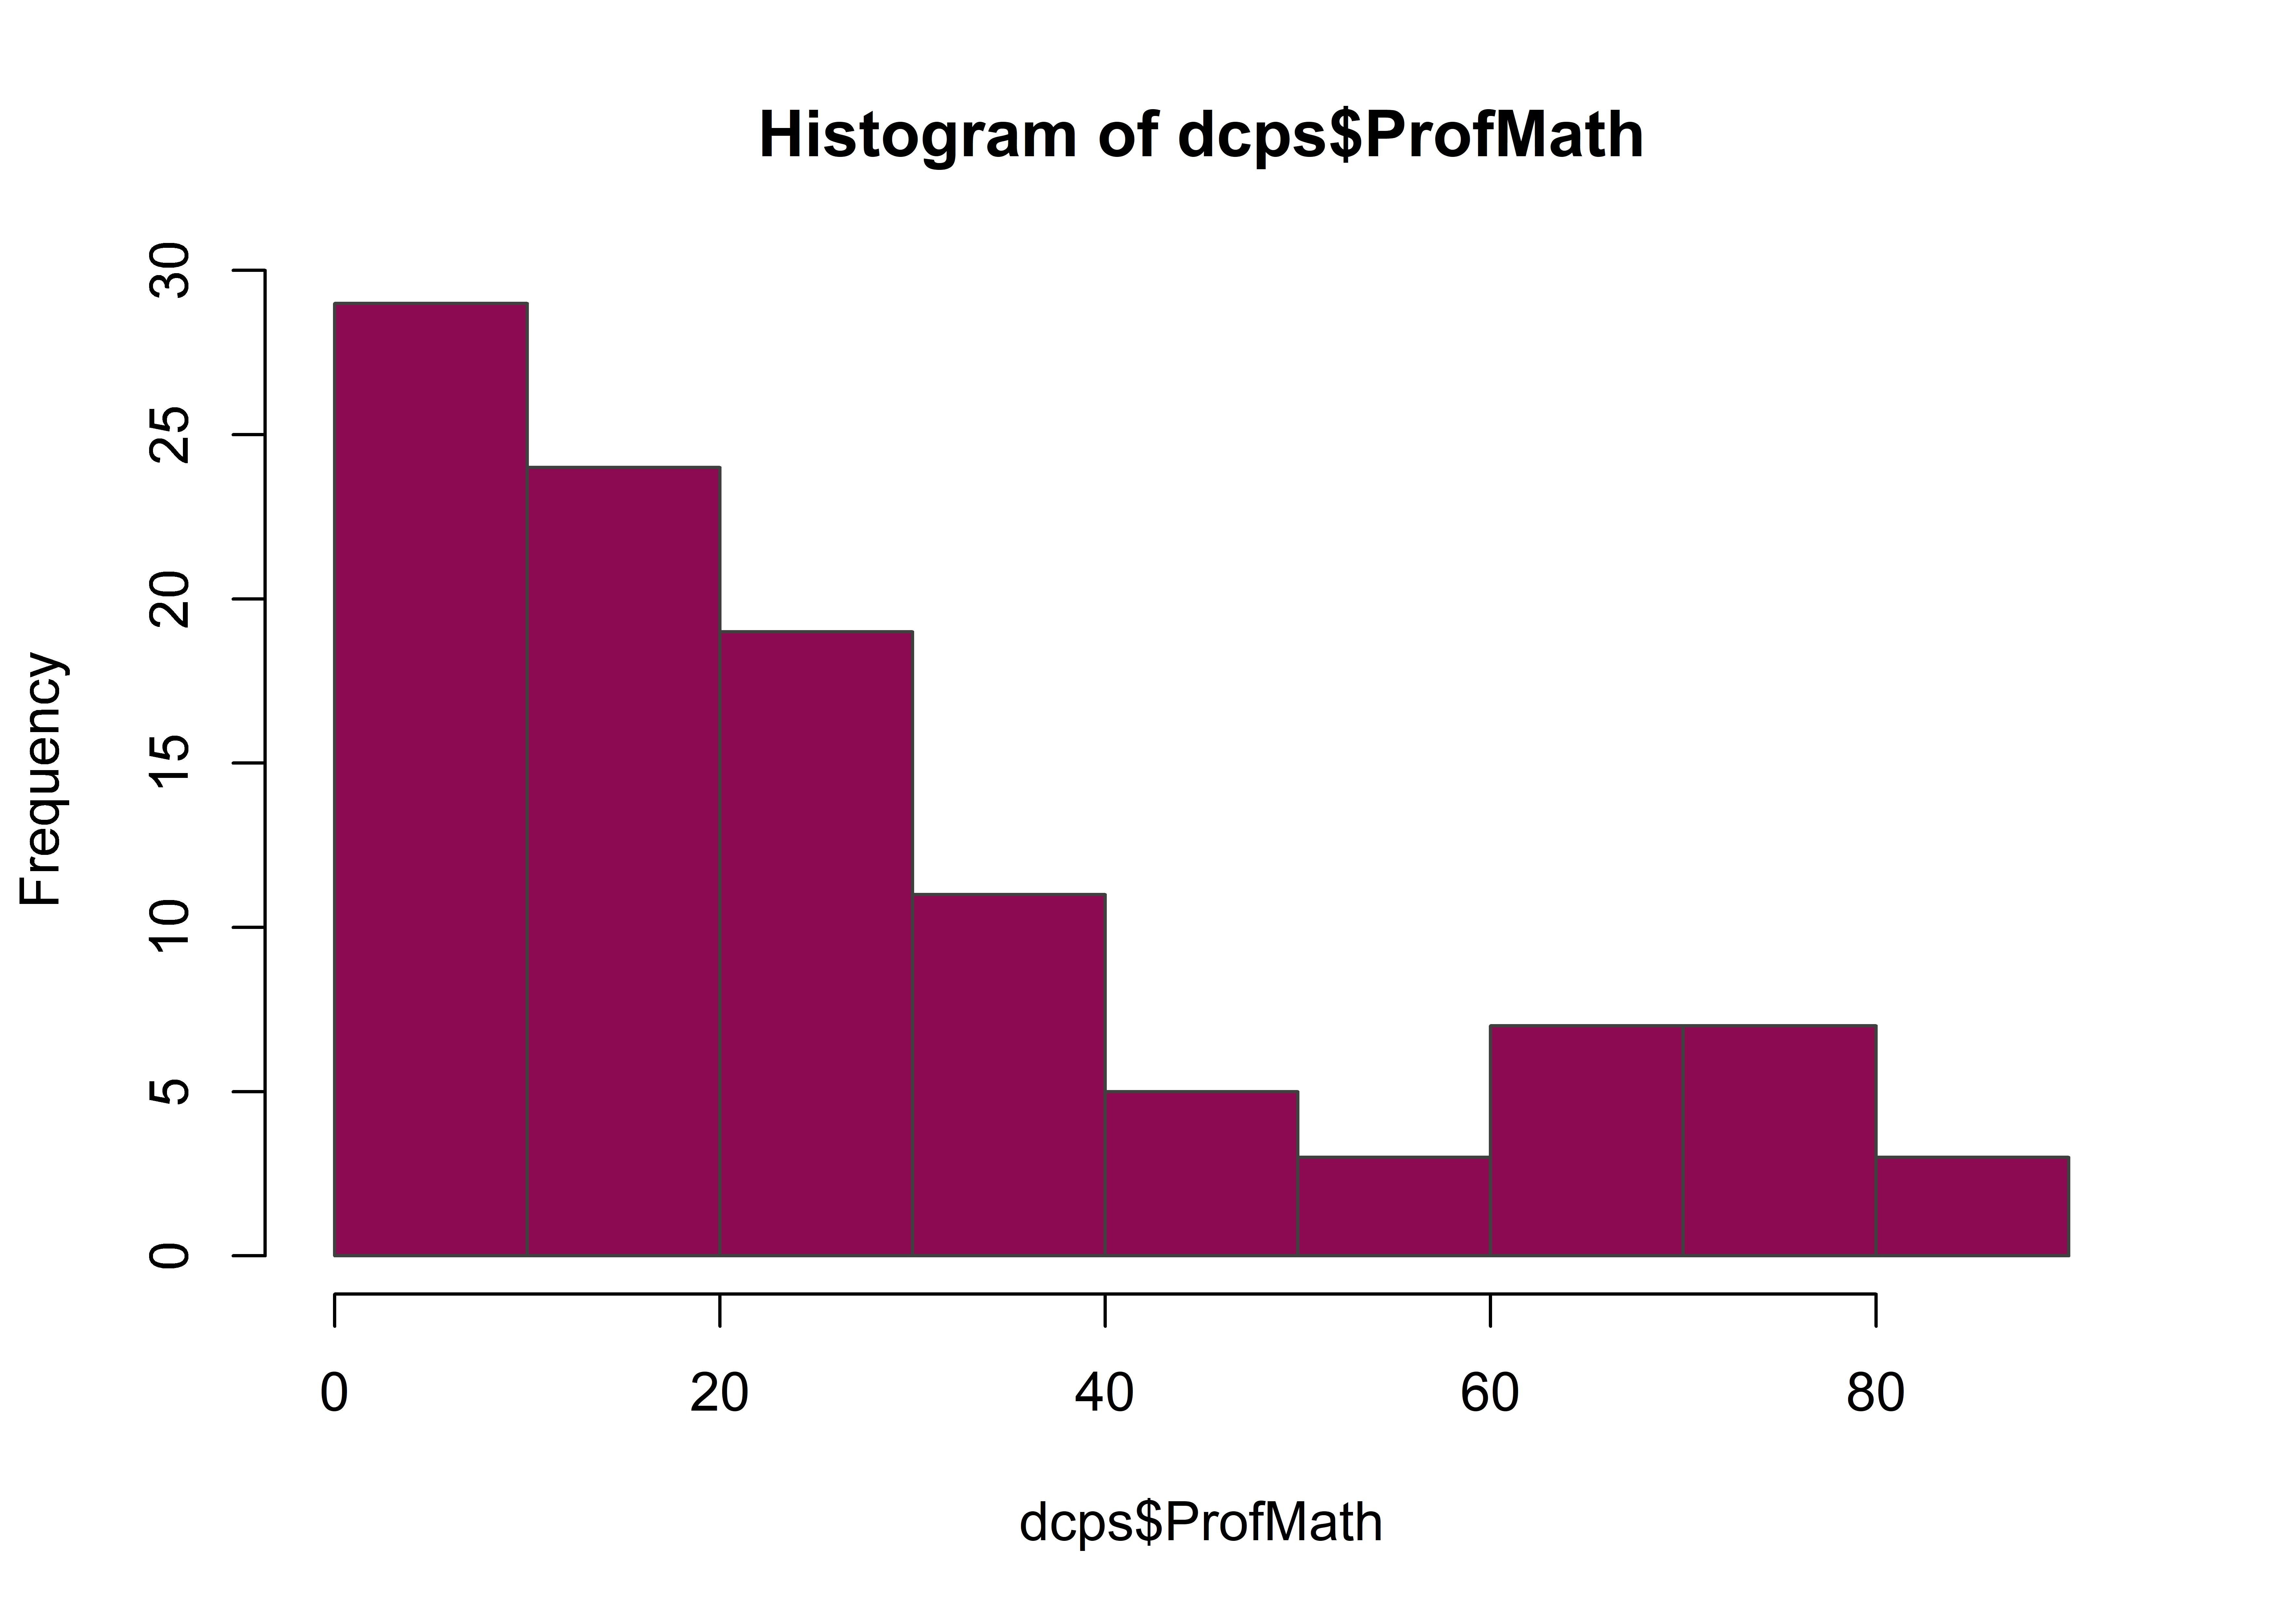
\includegraphics[width=0.4\linewidth]{SurvivR_files/figure-latex/gparms-1} \end{center}

\begin{Shaded}
\begin{Highlighting}[]

\CommentTok{\# Scatter plots with fit}
  \FunctionTok{plot}\NormalTok{(ProfMath }\SpecialCharTok{\textasciitilde{}}\NormalTok{ ProfLang, }\AttributeTok{data =}\NormalTok{ dcps,}
       \AttributeTok{pch =} \DecValTok{24}\NormalTok{,    }\CommentTok{\# shape of the point}
       \AttributeTok{col =} \StringTok{\textquotesingle{}red\textquotesingle{}}\NormalTok{) }\CommentTok{\# point color}
  
  \FunctionTok{abline}\NormalTok{(}\FunctionTok{lm}\NormalTok{(ProfMath }\SpecialCharTok{\textasciitilde{}}\NormalTok{ ProfLang, }\AttributeTok{data =}\NormalTok{ dcps), }
         \AttributeTok{col =} \StringTok{\textquotesingle{}blue\textquotesingle{}}\NormalTok{,}
         \AttributeTok{lty =} \DecValTok{4}\NormalTok{, }\CommentTok{\# line type (1{-}6)}
         \AttributeTok{lwd =} \DecValTok{3}\NormalTok{) }\CommentTok{\# line width (3=triple width)}
\end{Highlighting}
\end{Shaded}

\begin{center}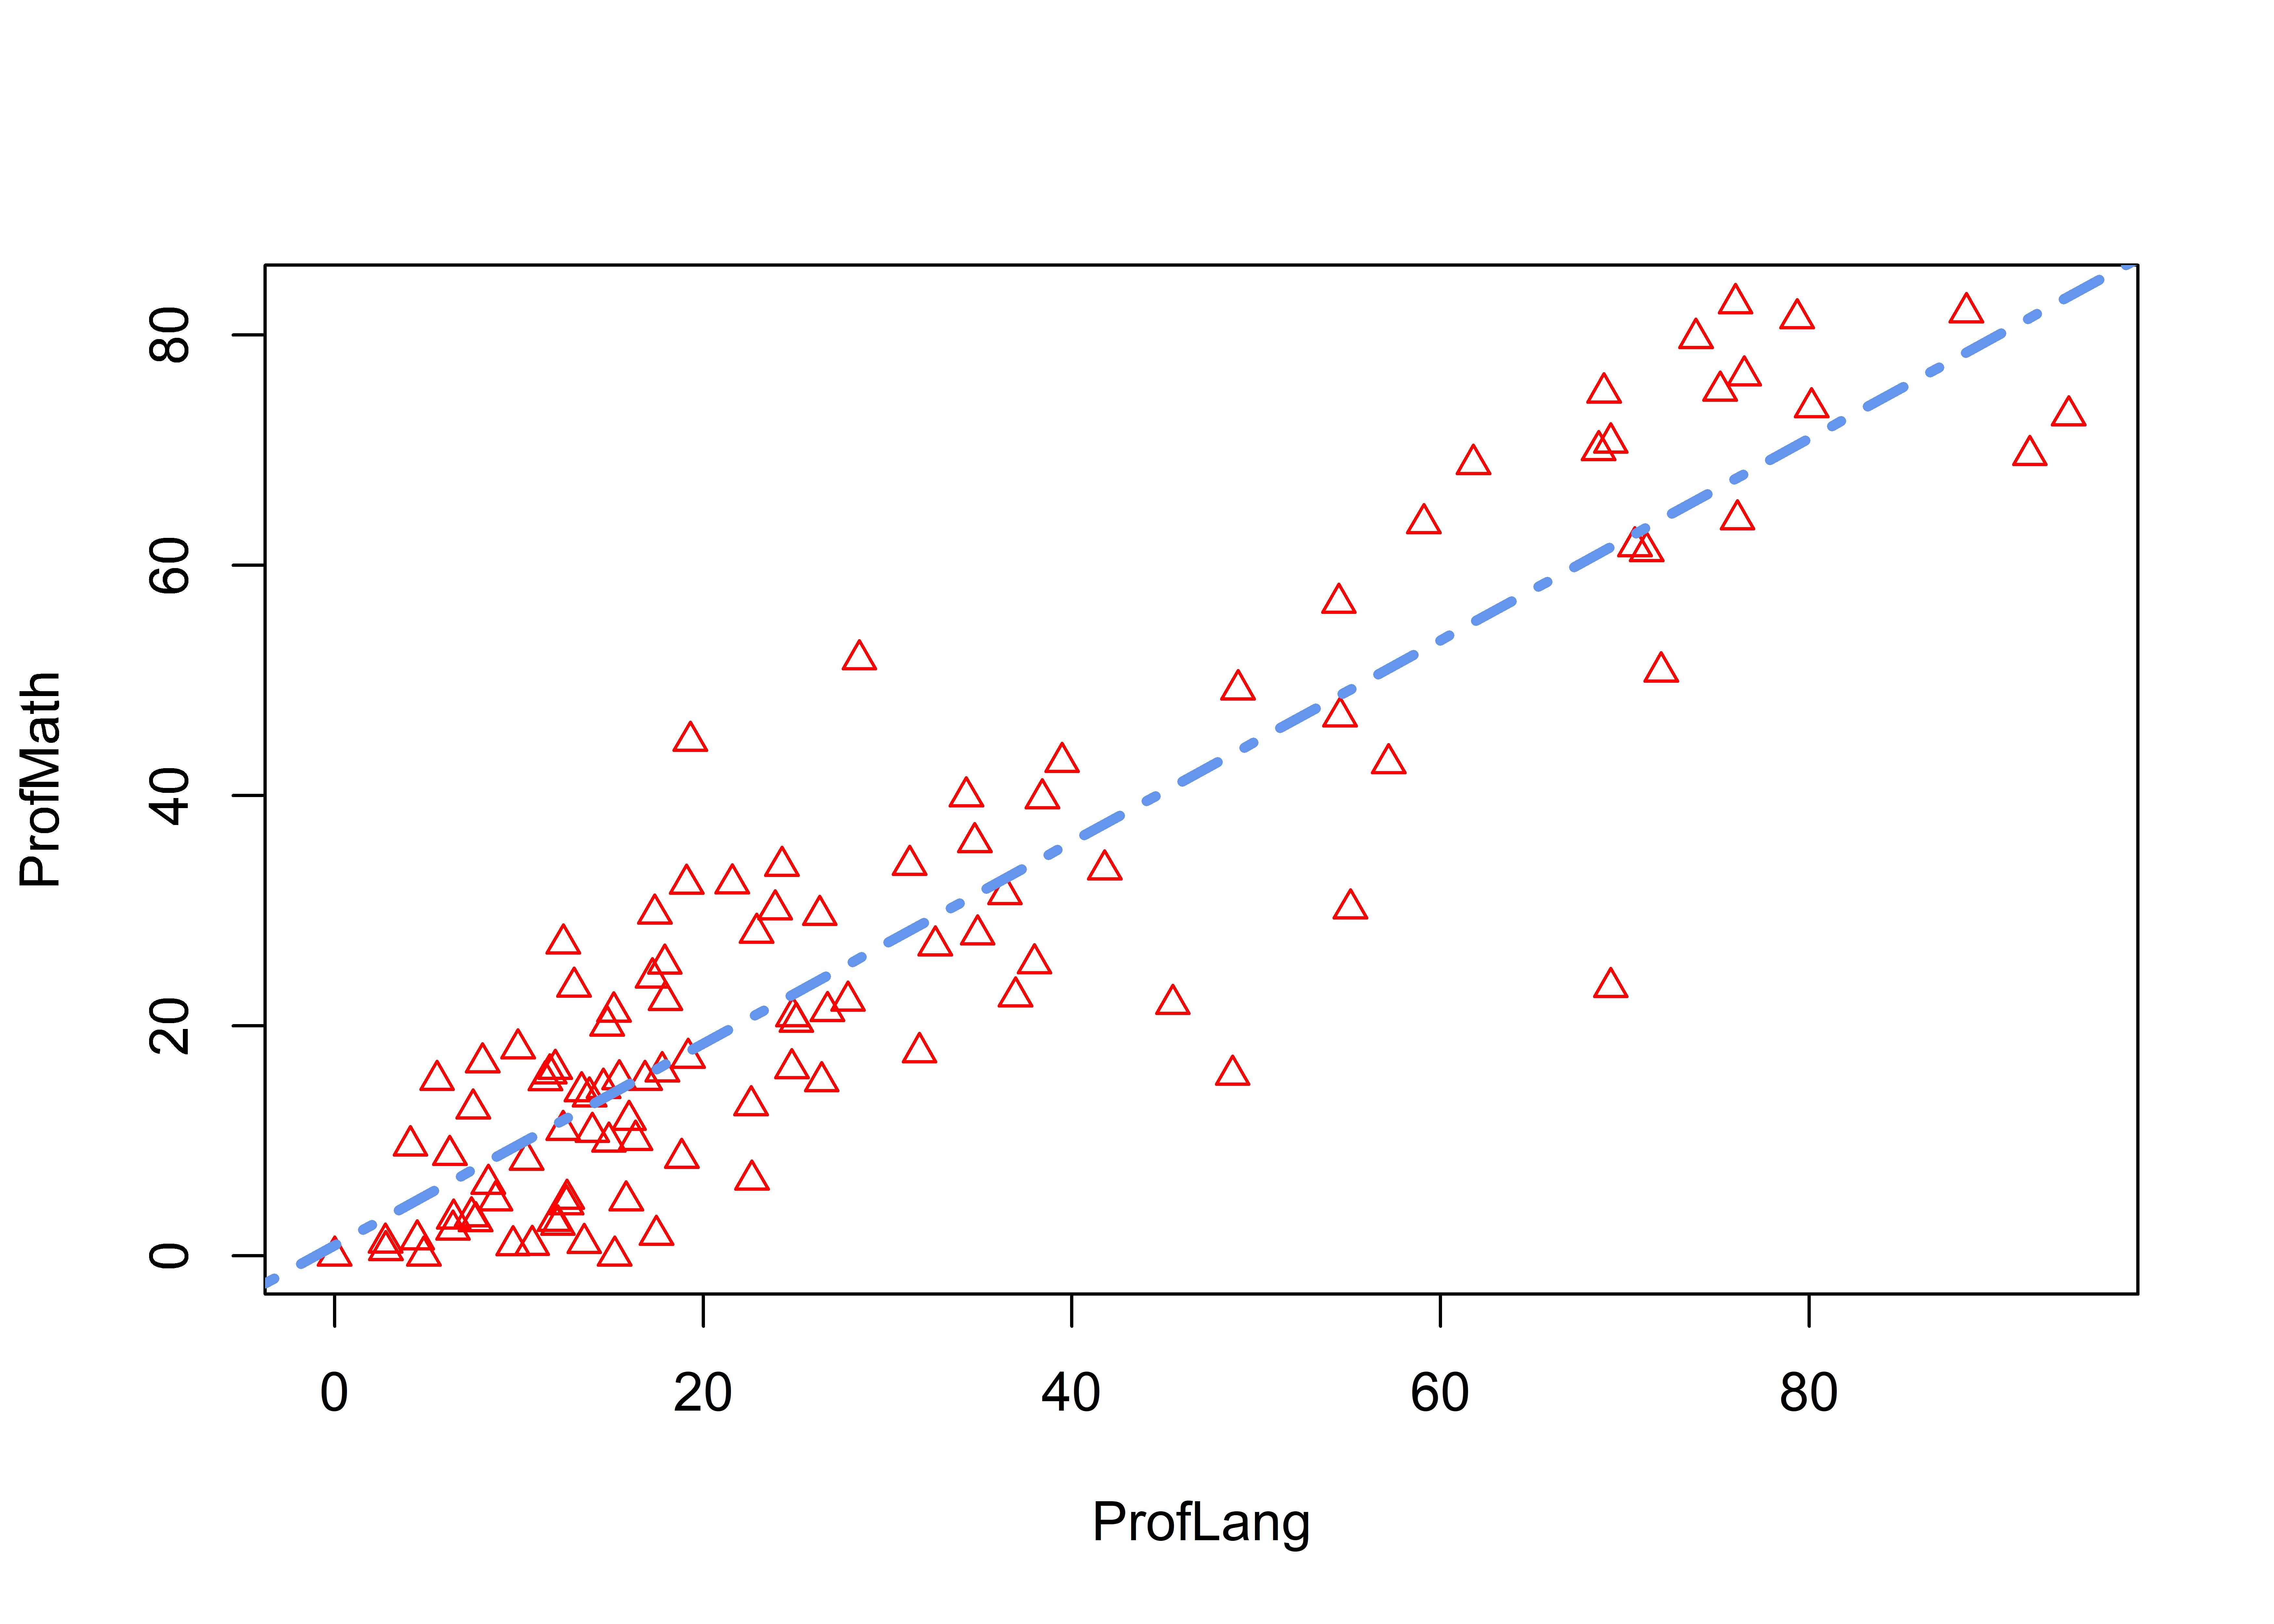
\includegraphics[width=0.4\linewidth]{SurvivR_files/figure-latex/gparms-2} \end{center}

\hypertarget{exportingsaving-graphs}{%
\section{Exporting/saving graphs}\label{exportingsaving-graphs}}

Once you have a formatted graph, it's time to export it. Find the \texttt{Export} button in the plot window and choose ``Save as Image'' (left-hand panel of the figure below). This opens the window shown in the right-hand panel. Here you want to select an appropriate format (typically \texttt{.jpeg}), name, and size. Size is crucial, and the target is the smallest possible without cutting out text. A size of 450x400 pixels is a pretty safe bet for most of what we do in this course.

\begin{figure}

{\centering 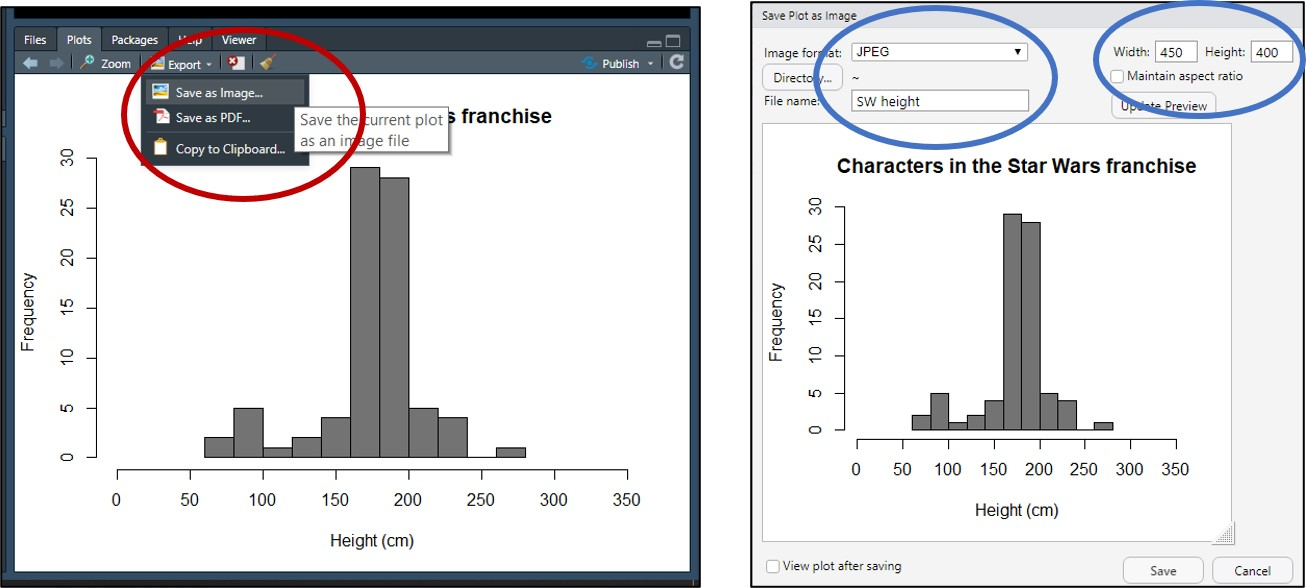
\includegraphics[width=0.85\linewidth]{C:\Users\ahart\Dropbox\SIS 600 AH\quick r survival guide\gphexport} 

}

\caption{Fortmat and export graphs}\label{fig:gphsave}
\end{figure}

  \bibliography{book.bib,packages.bib}

\printindex

\end{document}
